% =====================================================================
%  BÁO CÁO KỸ THUẬT — ĐỀ TÀI M8
%  Học đa nhiệm trên CIFAR-10: phân loại siêu lớp kết hợp dự đoán góc xoay
%  Biên dịch: tectonic -X compile main.tex     (hoặc: xelatex main.tex)
% =====================================================================
\documentclass[11pt,a4paper]{article}

% ---------- Ngôn ngữ và font (XeLaTeX / LuaLaTeX) ----------
% Bản Linux dùng STIX Two Text thay cho Times New Roman (Times New Roman là font
% Windows, không có trên Linux). STIX là thiết kế họ Times nên bám sát quy định
% trình bày học thuật Việt Nam, và hợp với STIX Two Math dùng cho công thức.
%
% Đã kiểm chứng bằng cách đọc trực tiếp bảng cmap của từng file font: đủ 91/91 ký tự
% có dấu dùng trong báo cáo, ở cả 4 mặt chữ (Regular/Bold/Italic/BoldItalic).
%
% Font được ĐÓNG GÓI KÈM trong report/assets/fonts/ và nạp bằng Path=, nên build
% được trên máy KHÔNG cài sẵn các font này. Vì Path= là đường dẫn tương đối, PHẢI
% biên dịch với thư mục làm việc là report/ (xem README mục 4).
%
% CẢNH BÁO: KHÔNG thay bằng Noto Serif / Noto Sans / Cantarell / Adwaita Sans —
% chúng là VARIABLE FONT và làm xdvipdfmx báo lỗi "Invalid font: -1".
% Caladea / Nimbus Roman / C059 thì THIẾU 59–62 ký tự tiếng Việt.
\usepackage{fontspec}
\usepackage{polyglossia}
\setdefaultlanguage{vietnamese}
\setotherlanguage{english}

% THÂN BÀI: Liberation Serif. Trước đây dùng STIX Two Text, nhưng cả STIX Two Text lẫn
% Carlito đều đặt dấu nặng (dấu chấm dưới) của ộ/ợ/ự/ậ/ệ QUÁ THẤP và tách rời khỏi chữ, còn
% dấu chồng hai tầng ở Ờ thì chồng lên nhau. Liberation Serif render các dấu này bám sát chữ.
% Thêm nữa Liberation Serif tương thích metric với Times New Roman, nên bản Linux trông khớp
% với bản Windows (main.tex dùng Times New Roman).
\setmainfont{LiberationSerif}[
  Path           = assets/fonts/liberation/,
  Extension      = .ttf,
  UprightFont    = *-Regular,
  BoldFont       = *-Bold,
  ItalicFont     = *-Italic,
  BoldItalicFont = *-BoldItalic,
]
% TIÊU ĐỀ: Liberation Sans thay Carlito — cùng lý do về dấu tiếng Việt. Ở trang bìa vốn
% dùng chữ in hoa có dấu chồng (TRƯỜNG, NGHỆ, THUẬT) nên lỗi của Carlito lộ rõ nhất.
\setsansfont{LiberationSans}[
  Path           = assets/fonts/liberation/,
  Extension      = .ttf,
  UprightFont    = *-Regular,
  BoldFont       = *-Bold,
  ItalicFont     = *-Italic,
  BoldItalicFont = *-BoldItalic,
]
\setmonofont{LiberationMono}[
  Path           = assets/fonts/mono/,
  Extension      = .ttf,
  UprightFont    = *-Regular,
  BoldFont       = *-Bold,
  ItalicFont     = *-Italic,
  BoldItalicFont = *-BoldItalic,
  Scale          = 0.86,
]

% Công thức: STIX Two Math. STIX được thiết kế để đi kèm Times, mà Liberation Serif chính là
% bản tương thích metric của Times New Roman, nên cặp này hài hoà. Công thức không chứa ký tự
% tiếng Việt nên không ảnh hưởng tới vấn đề dấu ở trên.
\usepackage{unicode-math}
\setmathfont{STIXTwoMath-Regular}[
  Path      = assets/fonts/stix/,
  Extension = .otf,
]

% ---------- Giãn dòng cho tiếng Việt ----------
% Tiếng Việt có dấu chồng hai tầng (ẫ ộ ự ỡ). Với giãn dòng đơn, dấu của dòng dưới
% ĐỤNG vào dòng trên và bị cắt cụt khi in — trông như "mất dấu". Chuẩn trình bày
% học thuật Việt Nam quy định giãn dòng 1,5. Ở đây dùng 1,25 để cân bằng giữa
% chất lượng dấu và giới hạn 15–25 trang của đề cương.
% (\setstretch thuộc gói setspace, nên PHẢI đặt SAU \usepackage{setspace}.)

% ---------- Trang và bố cục ----------
\usepackage[a4paper,top=2.5cm,bottom=2.5cm,left=2.8cm,right=2.3cm,headsep=0.6cm]{geometry}
\usepackage{fancyhdr}
\usepackage{setspace}
\setstretch{1.25}
\usepackage{parskip}
\usepackage{microtype}
\usepackage{ragged2e}
\usepackage{enumitem}
\usepackage{booktabs}
\usepackage{longtable}
\usepackage{tabularx}
\usepackage{multirow}
\usepackage{array}
\usepackage{makecell}
\usepackage{siunitx}
\usepackage{graphicx}
\usepackage{float}
\usepackage{caption}
\usepackage{subcaption}
\usepackage{xcolor}
\usepackage{tikz}
\usetikzlibrary{arrows.meta,positioning,calc,fit,backgrounds,shapes.geometric}
% unicode-math đã nạp ký hiệu toán; không dùng amssymb để tránh trùng lệnh \eth
\usepackage{amsmath}
\usepackage[most]{tcolorbox}
\usepackage{listings}
% csquotes không có style "vietnamese"; mặc định khi đó \enquote cho ra dấu ? vì
% glyph dấu ngoặc kép không được ánh xạ. Chọn style english để \enquote ra “ ”.
\usepackage[autostyle=true,style=english]{csquotes}
\usepackage[hidelinks,unicode]{hyperref}

% ---------- Ngưỡng tràn dòng chặt hơn mặc định ----------
% Cho phép giãn cách từ hơi rộng hơn để tránh Overfull \hbox trong bảng và danh mục.
\tolerance=2000
\emergencystretch=2em
\hbadness=3000
\vbadness=3000
\hfuzz=0.5pt

% ---------- Bảng màu ----------
\definecolor{m8blue}{HTML}{1F4E79}
\definecolor{m8teal}{HTML}{0F7B6C}
\definecolor{m8orange}{HTML}{C55A11}
\definecolor{m8gray}{HTML}{595959}
\definecolor{m8light}{HTML}{F2F5F8}
\definecolor{m8green}{HTML}{2C7A3F}
\definecolor{m8red}{HTML}{B03A2E}
% ---------- Màu nhận diện HCMUTE (lấy trực tiếp từ huy hiệu trường) ----------
% PHẢI trùng khớp với report/main.tex — hai file main dùng chung trang bìa.
\definecolor{hcmuteblue}{HTML}{283090}
\definecolor{hcmutered}{HTML}{E81820}
\definecolor{hcmutegray}{HTML}{4A4A4A}

\hypersetup{
  colorlinks=true,
  linkcolor=m8blue,
  citecolor=m8teal,
  urlcolor=m8orange,
  pdftitle={Hoc da nhiem tren CIFAR-10: phan loai sieu lop ket hop du doan goc xoay},
  pdfauthor={Dinh Xuan Huy}
}

% ---------- Tiêu đề / chú thích ----------
\captionsetup{font=small,labelfont={bf,color=m8blue},justification=justified,singlelinecheck=false}
\captionsetup[table]{skip=6pt}
\captionsetup[figure]{skip=6pt}

\pagestyle{fancy}
\fancyhf{}
\fancyhead[L]{\small\itshape Trí tuệ nhân tạo cho IoT — Đề tài M8}
\fancyhead[R]{\small\thepage}
\renewcommand{\headrulewidth}{0.4pt}
\fancypagestyle{plain}{\fancyhf{}\fancyfoot[C]{\small\thepage}\renewcommand{\headrulewidth}{0pt}}

% ---------- Định nghĩa hộp ----------
\newtcolorbox{keybox}[1][]{
  colback=m8light, colframe=m8blue, boxrule=0.6pt, arc=2pt,
  left=8pt, right=8pt, top=6pt, bottom=6pt, #1
}
\newtcolorbox{warnbox}[1][]{
  colback=orange!6, colframe=m8orange, boxrule=0.6pt, arc=2pt,
  left=8pt, right=8pt, top=6pt, bottom=6pt, #1
}
\newtcolorbox{resbox}[1][]{
  colback=green!5, colframe=m8green, boxrule=0.6pt, arc=2pt,
  left=8pt, right=8pt, top=6pt, bottom=6pt, #1
}
\newtcolorbox{limbox}[1][]{
  colback=gray!7, colframe=m8gray, boxrule=0.6pt, arc=2pt,
  left=8pt, right=8pt, top=6pt, bottom=6pt, #1
}

% ---------- Đoạn mã ----------
\lstdefinestyle{m8style}{
  basicstyle=\ttfamily\footnotesize,
  keywordstyle=\color{m8blue}\bfseries,
  commentstyle=\color{m8green}\itshape,
  stringstyle=\color{m8orange},
  numbers=left, numberstyle=\tiny\color{m8gray}, numbersep=8pt,
  frame=single, framerule=0.4pt, rulecolor=\color{m8gray!60},
  backgroundcolor=\color{gray!4},
  breaklines=true, breakatwhitespace=true, tabsize=4,
  showstringspaces=false, captionpos=b, language=Python,
}
\lstset{style=m8style}

% ---------- Lệnh dùng chung ----------
% Tên cấu hình (E1, E2-L, ...). KHÔNG dùng \textsc: cả Liberation Serif (bản Linux) lẫn
% Times New Roman (bản Windows) đều KHÔNG có mặt chữ small-caps, nên \textsc rơi vào shape
% `sc' không tồn tại, LaTeX phải thay bằng mặt chữ khác và cảnh báo
% "Font shape TU/.../m/sc undefined". Dùng sans đậm để tên cấu hình vẫn nổi bật trong thân
% bài serif mà không phụ thuộc tính năng tuỳ chọn của font.
\newcommand{\cfg}[1]{\textsf{\textbf{#1}}}
\newcommand{\DL}{D_{\mathrm{L}}}
\newcommand{\DU}{D_{\mathrm{U}}}
\newcommand{\Dtrain}{D_{\mathrm{train}}}
\newcommand{\Dval}{D_{\mathrm{val}}}
\newcommand{\Dtest}{D_{\mathrm{test}}}
\newcommand{\Lsup}{L_{\mathrm{sup}}}
\newcommand{\Lrot}{L_{\mathrm{rot}}}
% Loss mở rộng (E3--E6) — phải TRÙNG với report/main.tex.
\newcommand{\Lntxent}{L_{\mathrm{NT\text{-}Xent}}}
\newcommand{\Lsupcon}{L_{\mathrm{SupCon}}}
\newcommand{\Lcon}{L_{\mathrm{con}}}
\newcommand{\lamrot}{\lambda_{\mathrm{rot}}}
\newcommand{\lamc}{\lambda_{\mathrm{c}}}
\newcommand{\lam}{\lambda}
\newcommand{\enc}{f_{\theta}}
\newcommand{\gsup}{g_{\mathrm{sup}}}
\newcommand{\grot}{g_{\mathrm{rot}}}
\newcommand{\norm}{\mathcal{N}}
\newcommand{\code}[1]{\texttt{\small #1}}
\newcommand{\figref}[1]{Hình~\ref{#1}}
\newcommand{\tabref}[1]{Bảng~\ref{#1}}
\newcommand{\secref}[1]{mục~\ref{#1}}
\newcommand{\eqrefv}[1]{công thức~\eqref{#1}}

% Số liệu thực nghiệm do scripts/make_report_data.py sinh ra
% =====================================================================
%  SINH TỰ ĐỘNG bởi scripts/make_report_data.py — không sửa tay
% =====================================================================

\newcommand{\RRuns}{27}
\newcommand{\RExtRuns}{12}
\newcommand{\RTotalHours}{8,26}
\newcommand{\REnvPython}{3.12.10}
\newcommand{\REnvTorch}{2.11.0+cu128}
\newcommand{\REnvTorchvision}{0.26.0+cu128}
\newcommand{\REnvCudaBuild}{12.8}
\newcommand{\REnvGpu}{NVIDIA GeForce RTX 5070 Laptop GPU}
\newcommand{\REnvVram}{7,960}
\newcommand{\REnvCpu}{Intel64 Family 6 Model 197 Stepping 2, GenuineIntel}
\newcommand{\REnvCores}{16}
\newcommand{\REnvRam}{63,4}
\newcommand{\RParamInference}{11.169.858}
\newcommand{\RParamTraining}{11.171.910}
\newcommand{\RParamRotationHead}{2.052}
\newcommand{\RParamInferenceMiB}{42,61}
\newcommand{\RParamInferenceFileMiB}{42,68}
\newcommand{\RLatThreads}{4}
\newcommand{\RPreprocessMs}{0,132}
\newcommand{\RLatMeanCpu}{7,012}
\newcommand{\RLatMedianCpu}{6,866}
\newcommand{\RLatPNinetyFiveCpu}{9,466}
\newcommand{\RLatMeanGpu}{2,701}
\newcommand{\RLatMedianGpu}{2,062}
\newcommand{\RLatPNinetyFiveGpu}{5,870}
\newcommand{\REoneTenVal}{0,9319}
\newcommand{\REoneTenAcc}{0,9349}
\newcommand{\REoneTenConf}{0}
\newcommand{\REtwoTenDelta}{+1,51}
\newcommand{\REtwoTenDeltaStd}{0,06}
\newcommand{\REtwoTenDeltaPos}{3/3}
\newcommand{\REtwoLTenDelta}{$-$0,06}
\newcommand{\REtwoLTenDeltaStd}{0,38}
\newcommand{\REtwoLTenDeltaPos}{1/3}
\newcommand{\REtwoTenVal}{0,9470}
\newcommand{\REtwoLTenVal}{0,9313}
\newcommand{\REtwoTwentyDelta}{+1,34}
\newcommand{\REtwoTwentyDeltaStd}{0,18}
\newcommand{\REtwoTwentyDeltaPos}{3/3}
\newcommand{\REtwoLTwentyDelta}{+0,08}
\newcommand{\REtwoLTwentyDeltaStd}{0,05}
\newcommand{\REtwoLTwentyDeltaPos}{3/3}
\newcommand{\REoneTwentyVal}{0,9497}
\newcommand{\REoneTwentyAcc}{0,9517}
\newcommand{\REtwoTwentyVal}{0,9631}
\newcommand{\REtwoLTwentyVal}{0,9505}
\newcommand{\REtwoFiftyDelta}{+0,88}
\newcommand{\REtwoFiftyDeltaStd}{0,07}
\newcommand{\REtwoFiftyDeltaPos}{3/3}
\newcommand{\REtwoLFiftyDelta}{+0,55}
\newcommand{\REtwoLFiftyDeltaStd}{0,10}
\newcommand{\REtwoLFiftyDeltaPos}{3/3}
\newcommand{\REoneFiftyVal}{0,9690}
\newcommand{\REoneFiftyAcc}{0,9702}
\newcommand{\REtwoFiftyVal}{0,9777}
\newcommand{\REtwoLFiftyVal}{0,9745}
\newcommand{\RFindingSentence}{Ở cả ba lần lặp, cấu hình \cfg{E2} tại mức 10\,\% nhãn đều cho Macro-F1 test cao hơn \cfg{E1} (chênh lệch trung bình +1,51 điểm phần trăm, độ lệch chuẩn 0,06).}
\newcommand{\RFindingCone}{Ở cả ba lần lặp, cấu hình \cfg{E2} tại mức 10\,\% nhãn đều cho Macro-F1 test cao hơn \cfg{E1} (chênh lệch trung bình +1,51 điểm phần trăm, độ lệch chuẩn 0,06).}
\newcommand{\RFindingCtwo}{Mở rộng nguồn ảnh cho nhánh phụ: tại 10\,\% nhãn, \cfg{E2} cao hơn \cfg{E2-L} trung bình 1,57 điểm phần trăm (3/3 lần lặp dương); tại 20\,\% nhãn, \cfg{E2} cao hơn \cfg{E2-L} trung bình 1,25 điểm phần trăm (3/3 lần lặp dương); tại 50\,\% nhãn, \cfg{E2} cao hơn \cfg{E2-L} trung bình 0,32 điểm phần trăm (3/3 lần lặp dương).}
\newcommand{\RFindingCthree}{Tỷ lệ thời gian huấn luyện \cfg{E2}/\cfg{E1} là 10\,\%: $\times$1,68, 20\,\%: $\times$1,82, 50\,\%: $\times$1,99 (cùng 100 epoch, khác số lượt ảnh được xử lý mỗi bước).}
\newcommand{\RExtensionAnalysis}{Kết quả khối mở rộng: tại 10\,\% nhãn, cấu hình mở rộng tốt nhất là \cfg{E6}, cao hơn \cfg{E1} trung bình 2,60 điểm phần trăm (3/3 lần lặp dương). Đối chiếu hai loại loss contrastive — 10\,\% nhãn: SupCon (\cfg{E6}) so với NT-Xent (\cfg{E5}) chênh +0,83 điểm phần trăm, nghiêng về \cfg{E6}; 10\,\% nhãn: SupCon (\cfg{E4}) so với NT-Xent (\cfg{E3}) chênh +0,88 điểm phần trăm, nghiêng về \cfg{E4}. Khi đã có nhánh contrastive — 10\,\% nhãn: thêm nhánh xoay (\cfg{E6} so với \cfg{E4}) chênh +0,52 điểm phần trăm về phía \cfg{E6}; 10\,\% nhãn: thêm nhánh xoay (\cfg{E5} so với \cfg{E3}) chênh +0,58 điểm phần trăm về phía \cfg{E5}.}
\newcommand{\RExtensionConclusion}{Trong điều kiện đã khảo sát, cấu hình mở rộng \textbf{có} cải thiện so với \cfg{E1}: \cfg{E6} tại 10\,\% nhãn đạt chênh lệch trung bình +2,60 điểm phần trăm và dương ở cả 3/3 lần lặp. Tuy nhiên mức cải thiện này vẫn nằm trong cùng bậc độ lớn với độ lệch chuẩn giữa các lần lặp, nên chỉ được coi là bằng chứng thăm dò. Cần nhấn mạnh ba lần lặp chỉ cho bằng chứng ban đầu: không có tuyên bố ý nghĩa thống kê nào được đưa ra, và kết luận chỉ áp dụng cho kiến trúc, hai siêu lớp, các mức nhãn và giao thức đã khảo sát.}
\newcommand{\RIncomplete}{}


\begin{document}
\justifying

% =====================================================================
%  Trang bìa
% =====================================================================
\begin{titlepage}
\centering
\vspace*{0.4cm}

{\sffamily\bfseries\large TRƯỜNG ĐẠI HỌC CÔNG NGHỆ KỸ THUẬT\\[2pt]
THÀNH PHỐ HỒ CHÍ MINH\par}

\vspace{0.5cm}
{\color{m8blue}\rule{\textwidth}{1.2pt}}
\vspace{0.6cm}

{\sffamily\bfseries HỌC PHẦN: TRÍ TUỆ NHÂN TẠO CHO IoT\par}

\vspace{1.0cm}
{\sffamily\bfseries\Large ĐỀ CƯƠNG TIỂU LUẬN CUỐI KHÓA\par}
\vspace{0.5cm}
{\sffamily\bfseries\LARGE\color{m8blue}
HỌC ĐA NHIỆM TRÊN CIFAR-10:\\[4pt]
PHÂN LOẠI SIÊU LỚP KẾT HỢP\\[4pt]
DỰ ĐOÁN GÓC XOAY ẢNH TỰ GIÁM SÁT\par}

\vspace{0.7cm}
{\itshape\large Đánh giá trong điều kiện hạn chế nhãn huấn luyện\par}

\vspace{0.3cm}
{\color{m8blue}\rule{\textwidth}{0.8pt}}
\vspace{1.4cm}

\begin{tabular}{@{}p{5.2cm}@{\hspace{0.3cm}}l@{}}
\textbf{Mã đề tài:} & M8 \\[6pt]
\textbf{Sinh viên thực hiện:} & Đinh Xuân Huy \\[6pt]
\textbf{Mã số sinh viên:} & 23110102 \\[6pt]
\textbf{Phân nhóm:} & Đa nhiệm \\[6pt]
\textbf{Dữ liệu:} & CIFAR-10 \\[6pt]
\textbf{Lớp học phần:} & Trí tuệ nhân tạo cho IoT \\[6pt]
\textbf{Giảng viên hướng dẫn:} & \dotfill \\[6pt]
\textbf{Năm học:} & 2026--2027 \\
\end{tabular}

\vfill

\begin{minipage}{0.86\textwidth}
\begin{keybox}
\small\centering
\textbf{Báo cáo kỹ thuật bàn giao.} Toàn bộ số liệu Macro-F1, Accuracy, thời gian huấn luyện,
số tham số và độ trễ suy luận trong báo cáo này được sinh trực tiếp từ \RRuns{} lượt huấn luyện
thật trên môi trường được khai báo tại \secref{sec:env}. Mã nguồn, notebook, tệp cấu hình và
chỉ mục split/subset đi kèm gói tái lập.
\end{keybox}
\end{minipage}

\vspace{1.0cm}
{\sffamily\bfseries Thành phố Hồ Chí Minh, 2026\par}
\vspace{0.3cm}
\end{titlepage}

% =====================================================================
%  Tóm tắt
% =====================================================================
\section*{Tóm tắt}
\addcontentsline{toc}{section}{Tóm tắt}

\RIncomplete

\noindent
Báo cáo này trình bày một quy trình thực nghiệm có thể tái lập để đánh giá ảnh hưởng của
một \emph{nhiệm vụ phụ tự giám sát} đối với bài toán phân loại ảnh khi ngân sách nhãn bị
giới hạn. Cụ thể, CIFAR-10 được gộp thành hai siêu lớp do đề tài quy ước là
\emph{Animal} (6 lớp gốc) và \emph{Vehicle} (4 lớp gốc); một encoder ResNet-18 điều chỉnh cho
ảnh $32 \times 32$ được dùng chung cho hai đầu ra: phân loại siêu lớp có giám sát và dự đoán
góc xoay $k \in \{0,1,2,3\}$ được sinh tự động bằng \code{torch.rot90}. Nhãn của nhiệm vụ
phụ không cần nhãn ngữ nghĩa, nên nhánh xoay có thể khai thác thêm phần ảnh đã bị ẩn nhãn
của tập huấn luyện.

Khối thực nghiệm chính gồm ba cấu hình (\cfg{E1} baseline chỉ học siêu lớp, \cfg{E2-L} thêm
nhánh xoay nhưng chỉ dùng ảnh có nhãn, \cfg{E2} thêm nhánh xoay và dùng toàn bộ $\Dtrain$),
ba mức tỷ lệ nhãn ($10\,\%$, $20\,\%$, $50\,\%$) và ba lần lặp ghép cặp, tổng cộng \RRuns{}
lượt huấn luyện, mỗi lượt 100 epoch với tổng thời gian huấn luyện \RTotalHours{} giờ.
Chỉ số chính là Macro-F1 trên toàn bộ 10.000 ảnh test; Accuracy, precision/recall/F1 từng lớp
và ma trận nhầm lẫn được báo cáo kèm theo.

\medskip
\noindent\textbf{Kết quả chính.}
Tại mức nhãn $10\,\%$, Macro-F1 trên tập test đạt \REoneTenVal{} cho \cfg{E1} và \REtwoTenVal{}
cho \cfg{E2} (chênh lệch ghép cặp trung bình \REtwoTenDelta{} điểm phần trăm); tại mức
$50\,\%$ nhãn, \cfg{E1} đạt \REoneFiftyVal{} và \cfg{E2} đạt \REtwoFiftyVal{}
(chênh lệch \REtwoFiftyDelta{} điểm phần trăm). \RFindingSentence

\medskip
\noindent\textbf{Đóng góp có thể kiểm chứng.}
(i)~Một phép chia benchmark được đóng băng (seed 2026) với các tập nhãn lồng nhau
$\DL^{(10\%)} \subset \DL^{(20\%)} \subset \DL^{(50\%)}$ và chỉ mục đầy đủ được lưu lại;
(ii)~một giao thức kiểm tra việc che nhãn ở mức chỉ mục, bảo đảm nhãn thật của $\DU$ không
đi vào loss, không dùng để chọn positive pair và không tham gia chọn checkpoint;
(iii)~một khối kết quả ghép cặp theo lần lặp với chênh lệch $\Delta_s$ và độ lệch chuẩn
tường minh, kèm phân tích trường hợp không cải thiện;
(iv)~cài đặt đầy đủ \emph{bốn} cấu hình mở rộng contrastive \cfg{E3}--\cfg{E6} (NT-Xent và
SupCon) với siêu tham số $\lambda_c$ được khóa \emph{chỉ bằng validation} qua một quy trình
hai bước tách bạch thông tin;
(v)~các phép đo chi phí huấn luyện và suy luận được tách riêng, với kết luận về IoT được
giới hạn đúng theo thiết bị đã đo.

\medskip
\noindent\textbf{Kết quả phần mở rộng contrastive.}
\RExtensionConclusion

\medskip
\noindent\textbf{Giới hạn.}
Kết luận chỉ áp dụng cho phép gộp hai siêu lớp, các tỷ lệ nhãn và giao thức đã khảo sát.
Ba lần lặp chỉ cung cấp bằng chứng ban đầu về độ ổn định, không đủ để khẳng định ý nghĩa
thống kê. Kết quả đo độ trễ trên CPU của máy tính dùng để huấn luyện không phải là bằng chứng
về khả năng triển khai trên vi điều khiển. Không có kết quả nào trong báo cáo này được suy ra
từ số liệu minh họa.


\clearpage
\tableofcontents
\listoffigures
\listoftables
\clearpage

% =====================================================================
\section{Đặt vấn đề và mục tiêu}
\label{sec:intro}
% =====================================================================

\subsection{Đặt vấn đề}
\label{sec:intro-problem}

Bài toán được khảo sát là phân loại ảnh CIFAR-10 vào hai siêu lớp do đề tài quy ước:
\emph{Animal} và \emph{Vehicle}. Mô hình dùng chung một bộ trích xuất đặc trưng ResNet-18 và
đồng thời học hai nhiệm vụ: nhiệm vụ chính là phân loại siêu lớp có giám sát, nhiệm vụ phụ là
dự đoán phép xoay đã được áp dụng lên ảnh. Nhãn của nhiệm vụ phụ được sinh tự động từ chính
phép biến đổi, nhờ đó không cần nhãn ngữ nghĩa của ảnh~\cite{he2016resnet,gidaris2018rotnet}.

Động cơ nghiên cứu không nằm ở việc đề xuất một kiến trúc mới, mà ở việc \emph{đánh giá khả
năng khai thác tín hiệu tự giám sát khi số ảnh có nhãn dùng cho huấn luyện bị giới hạn}.
Nhiệm vụ dự đoán góc xoay được vận dụng từ hướng nghiên cứu RotNet; việc ghép ResNet-18 với
hai đầu ra không được xem là đóng góp kiến trúc. Cần nhấn mạnh một điểm dễ gây nhầm lẫn:
\emph{góc xoay ở đây là góc biến đổi nhân tạo}, không phải góc tư thế thực của đối tượng
trong ảnh~\cite{gidaris2018rotnet}.

Ở cấu hình có sử dụng thêm ảnh không nhãn, thiết lập thực chất là \emph{học bán giám sát} với
một nhiệm vụ phụ tự giám sát. Thuật ngữ \enquote{học đa nhiệm} mô tả giai đoạn huấn luyện;
khi suy luận, hệ thống chỉ giữ nhiệm vụ phân loại Animal/Vehicle. Vì vậy lợi ích cần kiểm
chứng là \emph{chất lượng phân loại}, chứ không phải mặc nhiên là giảm chi phí suy luận so với
một mô hình đơn nhiệm có cùng backbone.

Ba câu hỏi đánh giá được dùng xuyên suốt báo cáo:

\begin{table}[htbp]
  \centering
  \small
  \begin{tabular}{@{}p{4.6cm} p{10.4cm}@{}}
    \toprule
    Câu hỏi & Nội dung đánh giá \\
    \midrule
    C1 --- Hiệu quả phân loại &
    M8 có thay đổi Macro-F1 và Accuracy so với baseline chỉ học phân loại siêu lớp trong cùng
    ngân sách nhãn hay không? \\
    \addlinespace
    C2 --- Vai trò của dữ liệu &
    Kết quả khác nhau thế nào khi nhánh rotation chỉ dùng ảnh thuộc tập có nhãn và khi được
    dùng toàn bộ tập train? \\
    \addlinespace
    C3 --- Chi phí thực hiện &
    Chi phí huấn luyện tăng bao nhiêu; mô hình một đầu ra khi suy luận có số tham số, dung
    lượng và độ trễ như thế nào trên máy đo xác định? \\
    \bottomrule
  \end{tabular}
  \caption{Ba câu hỏi đánh giá và nội dung tương ứng. Câu C1 và C2 được trả lời bằng khối
  thực nghiệm chính (\secref{sec:results-main}); câu C3 bằng các phép đo chi phí ở
  \secref{sec:results-cost}.}
  \label{tab:questions}
\end{table}

\subsection{Mục tiêu và câu hỏi nghiên cứu}
\label{sec:intro-goal}

\textbf{Mục tiêu tổng quát.} Xây dựng và đánh giá một quy trình thực nghiệm có thể tái lập để
xác định ảnh hưởng của nhiệm vụ dự đoán góc xoay đối với phân loại siêu lớp tại các mức
$10\,\%$, $20\,\%$ và $50\,\%$ nhãn huấn luyện.

\textbf{Mục tiêu mở rộng.} Đề cương giữ hướng Contrastive Learning/SupCon ở phần \emph{mở rộng
tùy chọn} (các cấu hình \cfg{E3}--\cfg{E6}). Báo cáo này triển khai đầy đủ hướng đó và báo cáo
kết quả riêng tại \secref{sec:results-ext}, sau khi phần bắt buộc đã hoàn tất.

\textbf{Giả thuyết cần kiểm chứng.} Nhiệm vụ phụ \emph{có thể} cải thiện kết quả, đặc biệt khi
ít nhãn. Đây là một giả thuyết khoa học, không phải chỉ tiêu cam kết. Báo cáo phải trình bày
đầy đủ cả trường hợp không cải thiện hoặc suy giảm; không có yêu cầu nào buộc kết quả của M8
phải cao hơn baseline.

\begin{warnbox}
\textbf{Nguyên tắc báo cáo trung thực.} Mọi kết quả trong báo cáo này — kể cả kết quả âm —
đều được giữ nguyên như khi chạy thực nghiệm. Không có số liệu minh họa nào được đặt vào vị
trí kết quả thực nghiệm, và không có lượt chạy nào bị loại bỏ sau khi đã xem kết quả test.
Mục tiêu không được điều chỉnh sau khi biết kết quả.
\end{warnbox}

\subsection{Phạm vi}
\label{sec:intro-scope}

Giữ nguyên CIFAR-10, ResNet-18 điều chỉnh cho ảnh $32 \times 32$ và thời gian dự kiến bốn
tuần. Phần bắt buộc tập trung vào baseline và M8; Contrastive Learning/SupCon là mở rộng tùy
chọn, được triển khai và báo cáo ở \secref{sec:results-ext} nhưng \emph{không} thuộc tiêu chí
hoàn thành bắt buộc. Việc đánh giá chi phí suy luận phục vụ thảo luận về Edge AI, \emph{không
thay thế} thử nghiệm trên thiết bị IoT thực tế và \emph{không mặc nhiên} chứng minh khả năng
triển khai trên vi điều khiển.

\begin{limbox}
\textbf{Những gì báo cáo này không khẳng định:} (i)~không so sánh trực tiếp Accuracy hai lớp
với bảng xếp hạng CIFAR-10 mười lớp; (ii)~không khẳng định đặc trưng học được tổng quát hơn
hay thuật toán là mới; (iii)~không khẳng định tối ưu năng lượng; (iv)~không khẳng định đã xây
dựng một hệ thống IoT hoàn chỉnh.
\end{limbox}

% =====================================================================
\section{Tập dữ liệu và tiền xử lý}
\label{sec:data}
% =====================================================================

\subsection{Dữ liệu và ánh xạ nhãn}
\label{sec:data-mapping}

CIFAR-10 gồm 60.000 ảnh RGB kích thước $32 \times 32$: 50.000 ảnh train chính thức và 10.000
ảnh test chính thức; mỗi lớp gốc có 5.000 ảnh train và 1.000 ảnh test~\cite{krizhevsky2009cifar}.
Hai siêu lớp dưới đây là \emph{phép gộp của đề tài}, không phải bộ nhãn siêu lớp chính thức
của CIFAR-10. Việc ghi rõ điều này là cần thiết để tránh so sánh sai với các bảng xếp hạng
chuẩn.

\begin{table}[htbp]
  \centering
  \small
  \begin{tabular}{@{}c l l c@{}}
    \toprule
    Nhãn mới & Siêu lớp & Các lớp gốc & Số lớp gốc \\
    \midrule
    0 & Animal  & bird, cat, deer, dog, frog, horse & 6 \\
    1 & Vehicle & airplane, automobile, ship, truck & 4 \\
    \bottomrule
  \end{tabular}
  \caption{Ánh xạ từ 10 lớp gốc của CIFAR-10 sang hai siêu lớp của đề tài. Theo thứ tự nhãn gốc,
  Animal $= \{2,3,4,5,6,7\}$ và Vehicle $= \{0,1,8,9\}$.}
  \label{tab:label-map}
\end{table}

Sau ánh xạ, tỷ lệ Animal/Vehicle là $60\,\%/40\,\%$ và không còn cân bằng. Hệ quả trực tiếp:
một bộ phân loại luôn đoán \enquote{Animal} đã đạt Accuracy $60\,\%$ trên phép chia này, nên
Accuracy đơn lẻ không phản ánh chất lượng của lớp thiểu số. Do đó \textbf{Macro-F1 là chỉ số
chính} và Accuracy chỉ là chỉ số bổ sung~\cite{guo2017calibration}.

\figref{fig:dataset-samples} minh họa trực tiếp phép gộp này: mỗi hàng là một lớp gốc, màu
khung thể hiện siêu lớp mà lớp đó thuộc về. Hình cũng cho thấy vì sao bài toán không tầm
thường: cùng một siêu lớp chứa các đối tượng rất khác nhau (chim, mèo, hươu, chó, ếch, ngựa),
trong khi hai siêu lớp lại có thể trông gần giống nhau ở kích thước ảnh $32 \times 32$ — ví dụ
\emph{airplane} nằm trên nền trời xanh có thể bị nhầm với \emph{bird}.

\begin{figure}[htbp]
  \centering
  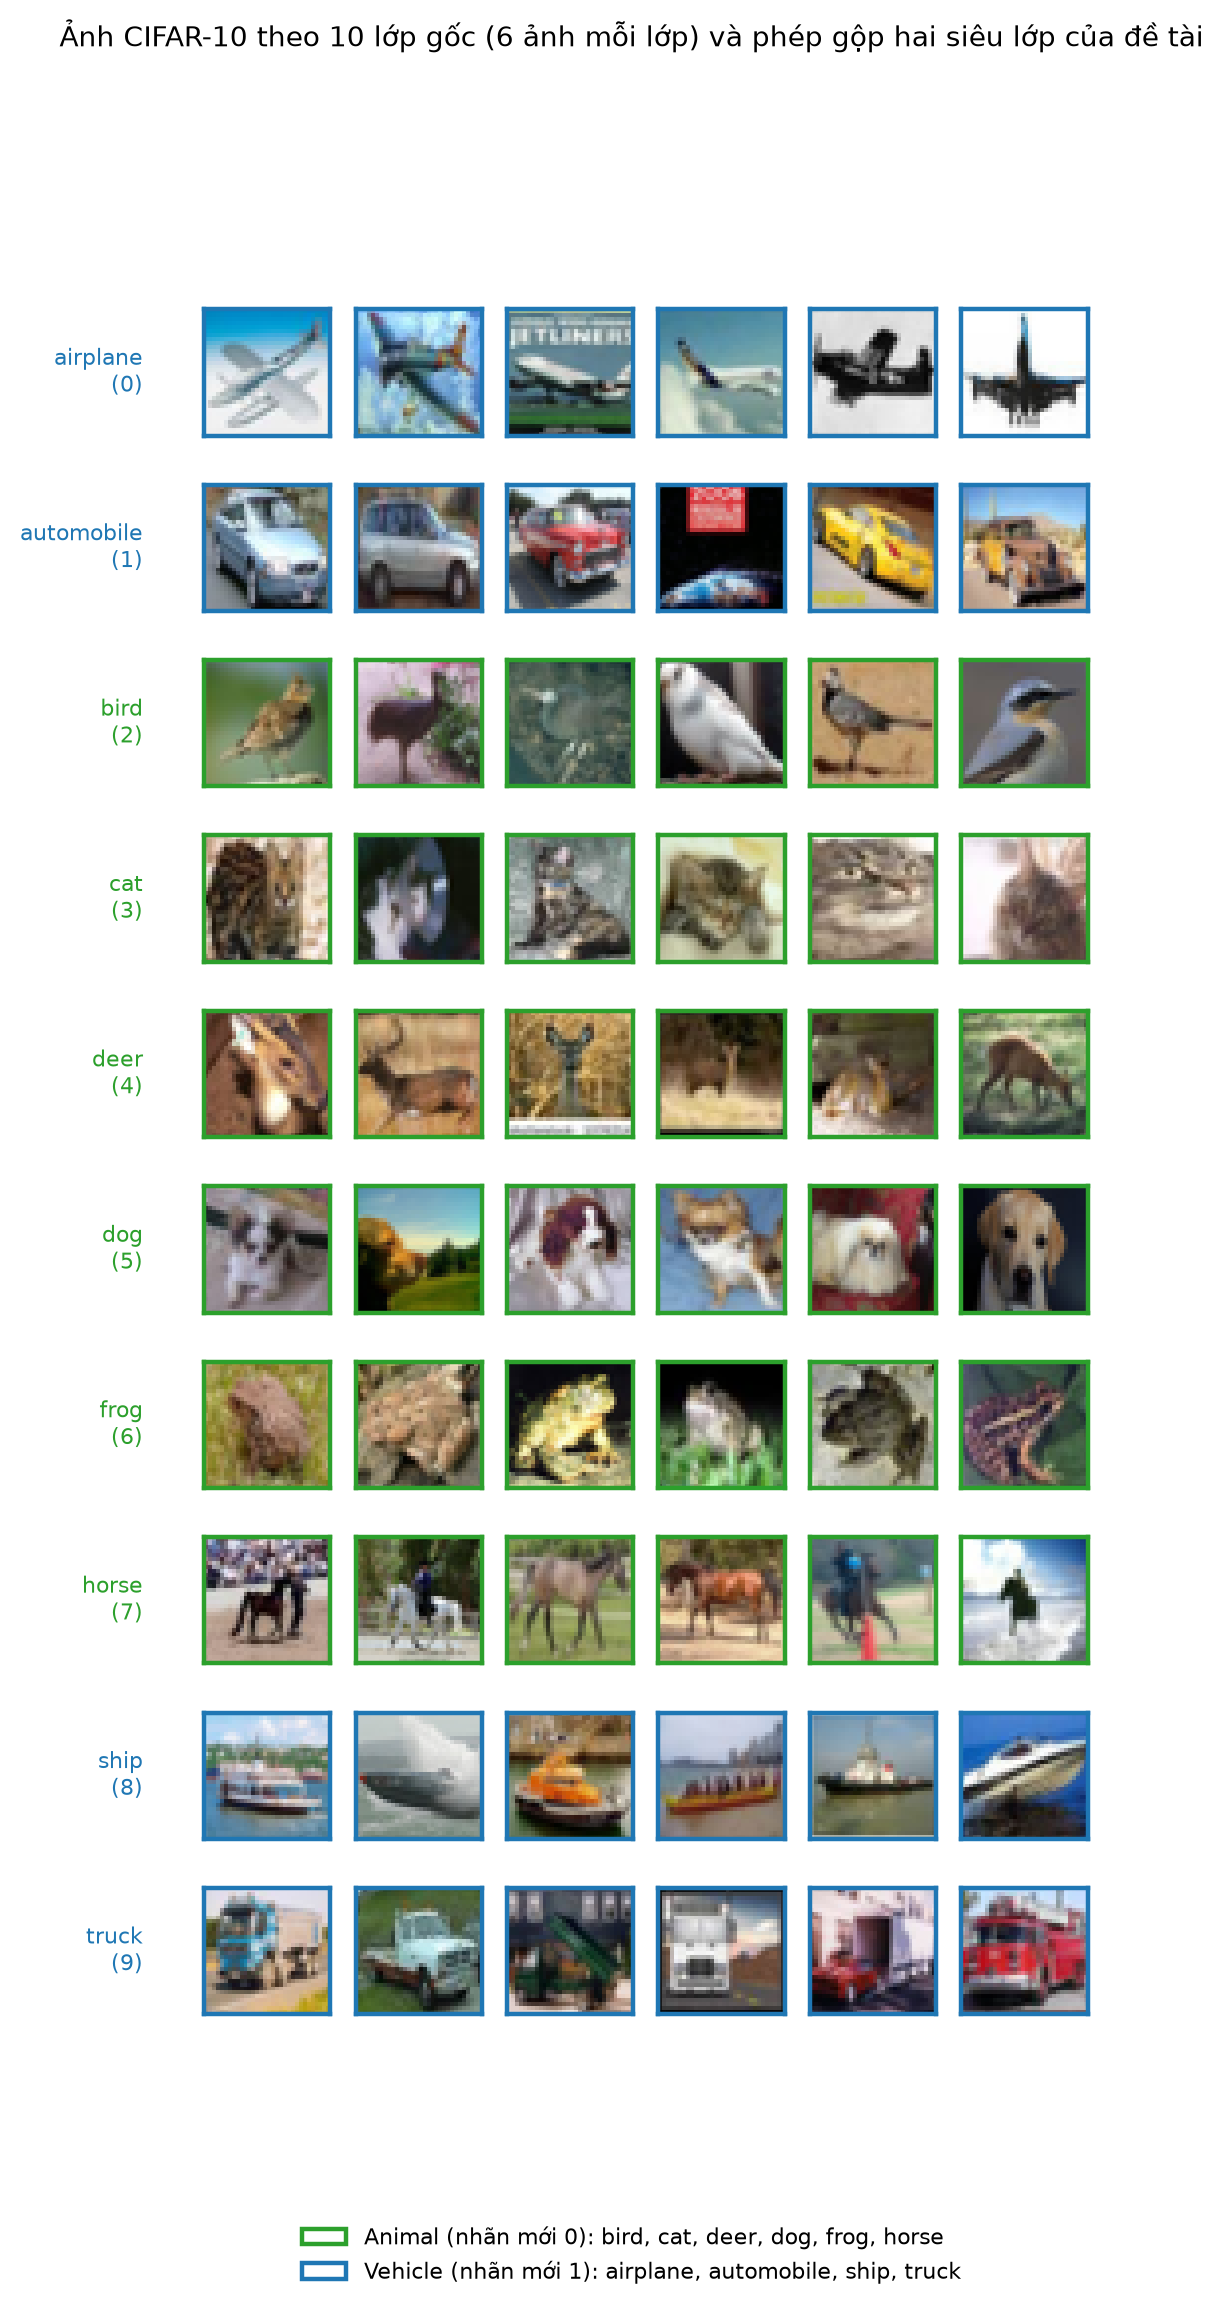
\includegraphics[width=\textwidth]{../results/figures/figA1_dataset_samples.png}
  \caption{Ảnh CIFAR-10 theo 10 lớp gốc (6 ảnh mỗi lớp, lấy ngẫu nhiên với seed 2026) và phép
  gộp hai siêu lớp của đề tài. Khung xanh lá = Animal (nhãn mới 0, gồm 6 lớp gốc);
  khung xanh dương = Vehicle (nhãn mới 1, gồm 4 lớp gốc). Số trong ngoặc là nhãn gốc của
  CIFAR-10.}
  \label{fig:dataset-samples}
\end{figure}

% Sinh tự động — scripts/make_report_data.py
\begin{table}[htbp]
  \centering
  \small
  \begin{tabular}{@{}l r r r r@{}}
    \toprule
    Tập & Tổng số ảnh & Animal & Vehicle & Tỷ lệ Animal \\
    \midrule
    $\Dtrain$ & 45.000 & 27.000 & 18.000 & 60{,}0\,\% \\
    $\Dval$   & 5.000  & 3.000  & 2.000  & 60{,}0\,\% \\
    $\Dtest$  & 10.000 & 6.000  & 4.000  & 60{,}0\,\% \\
    \bottomrule
  \end{tabular}
  \caption{Quy mô và thành phần của ba tập dữ liệu sau phép gộp siêu lớp. Tập test được giữ riêng hoàn toàn và chỉ mở ra ở bước đánh giá cuối cùng.}
  \label{tab:split}
\end{table}

\figref{fig:dataset-distribution} trình bày phân bố lớp trên ba tập. Panel~(a) xác nhận phép chia
phân tầng giữ đúng 5.000 ảnh train và 1.000 ảnh test cho mỗi lớp gốc; panel~(b) cho thấy tỷ lệ
$60/40$ được giữ nguyên trên cả $\Dtrain$, $\Dval$ và $\Dtest$ — điều này là cần thiết để chỉ số
trên validation còn dự báo được cho test; panel~(c) cho thấy ngân sách nhãn thay đổi thế nào
theo ba mức tỷ lệ.

\begin{figure}[htbp]
  \centering
  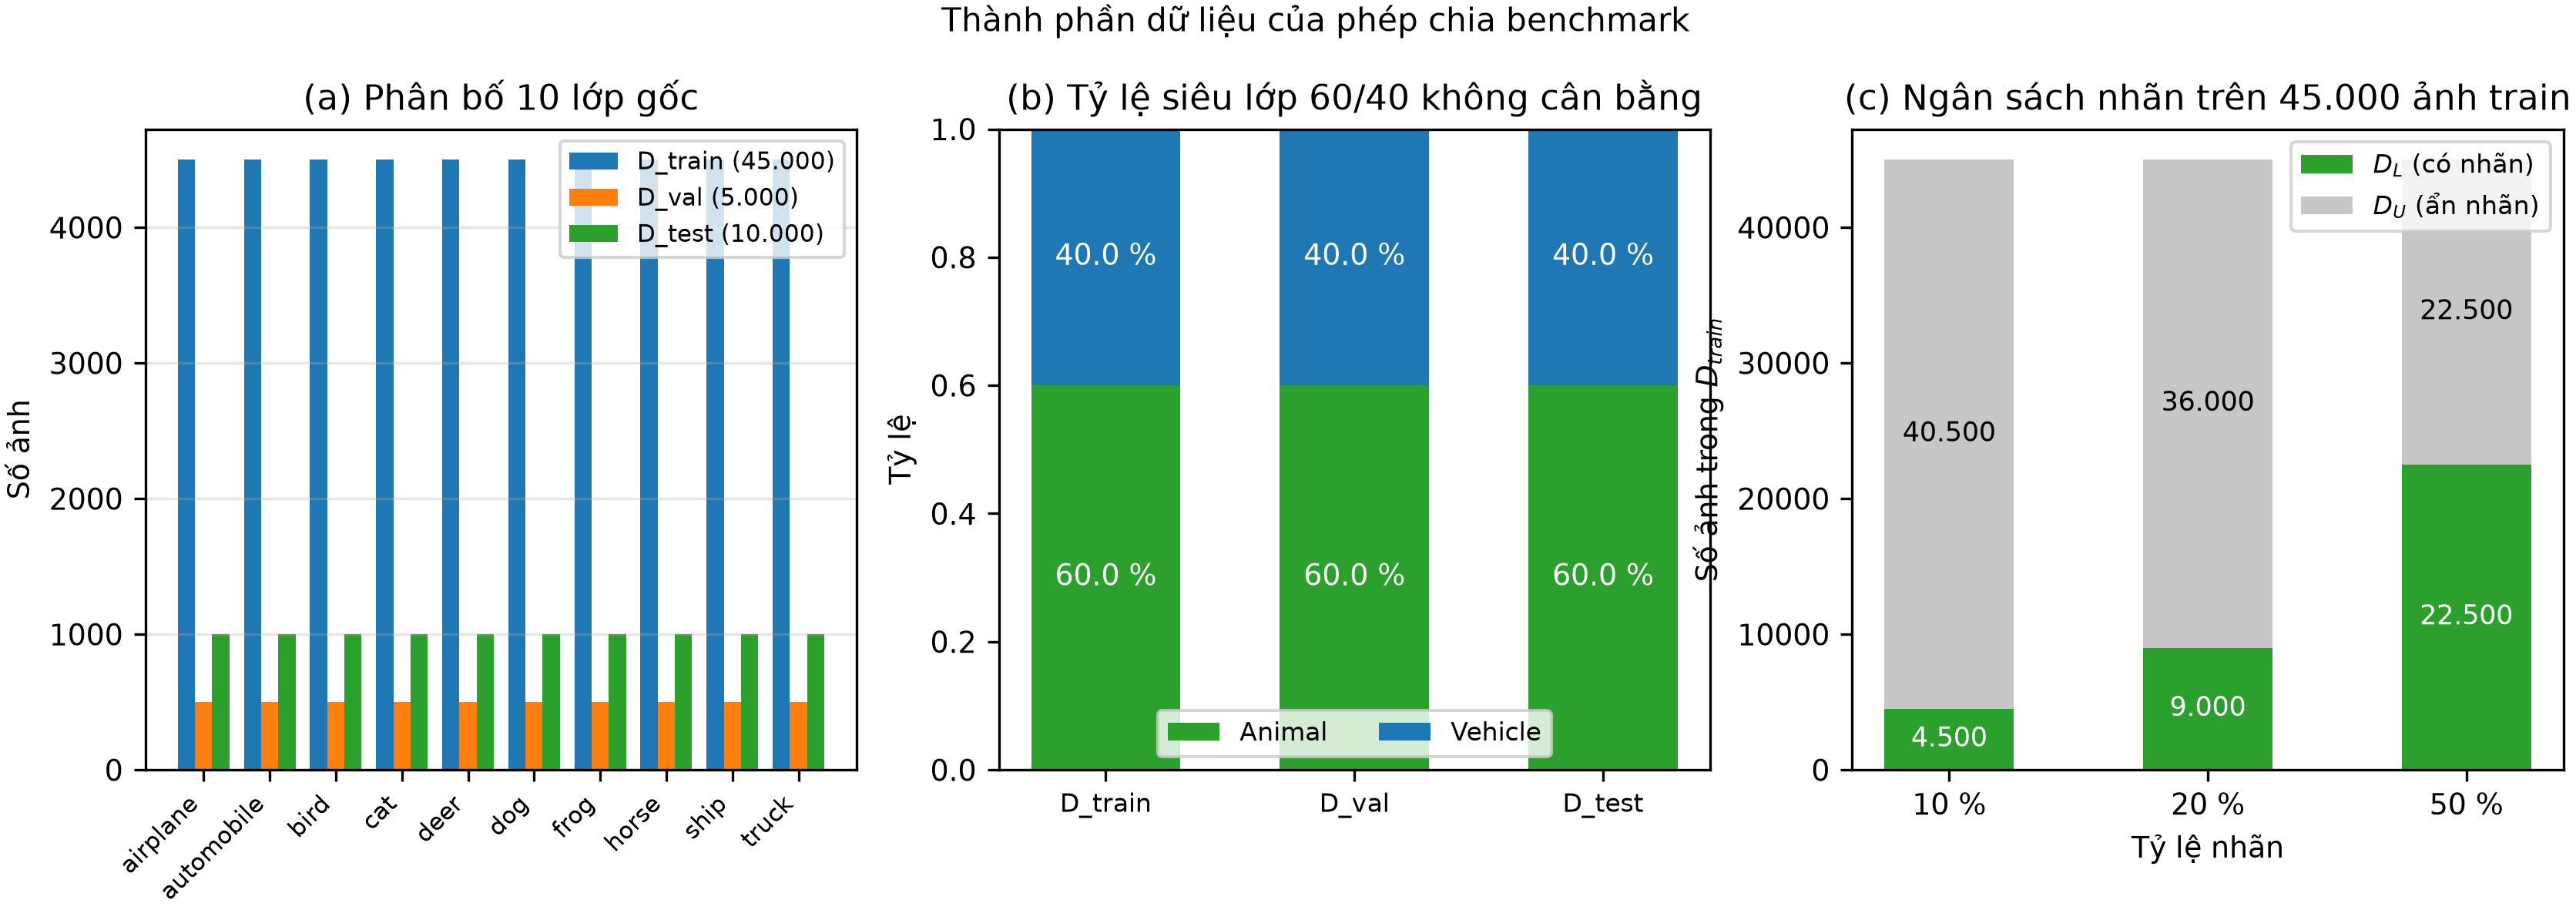
\includegraphics[width=\textwidth]{../results/figures/figA2_class_distribution.png}
  \caption{Thành phần dữ liệu của phép chia benchmark. (a)~Số ảnh mỗi lớp gốc trên ba tập;
  (b)~tỷ lệ hai siêu lớp $60/40$ trên ba tập; (c)~ngân sách nhãn: $\DL$ so với $\DU$ trên
  45.000 ảnh của $\Dtrain$.}
  \label{fig:dataset-distribution}
\end{figure}

\subsection{Chia dữ liệu và ngân sách nhãn}
\label{sec:data-split}

Quy trình chia dữ liệu được đóng băng trước khi huấn luyện và lưu đầy đủ chỉ mục:

\begin{enumerate}[label=\textbf{B\arabic*.},leftmargin=1.4cm,itemsep=3pt]
  \item Dùng seed $2026$ để chia 50.000 ảnh train thành $\Dtrain$ gồm 45.000 ảnh và $\Dval$
        gồm 5.000 ảnh, \emph{phân tầng theo 10 lớp gốc}. Kết quả phân tầng cho
        $\Dval = 3.000$ Animal $+ 2.000$ Vehicle.
  \item Tập test chính thức $\Dtest$ được giữ riêng hoàn toàn, không tham gia bất kỳ bước
        nào của quá trình thiết kế và lựa chọn phương pháp.
  \item Trong mỗi lần lặp $s \in \{42, 43, 44\}$, tạo một thứ tự ngẫu nhiên theo từng lớp gốc
        trên $\Dtrain$, rồi lấy các tập có nhãn \emph{lồng nhau}
        $\DL^{(10\%)} \subset \DL^{(20\%)} \subset \DL^{(50\%)}$.
  \item $\DU = \Dtrain \setminus \DL$ là phần ẩn nhãn; nhãn thật của $\DU$ bị chặn ở mức
        chỉ mục và không bao giờ được đọc trong quá trình huấn luyện.
\end{enumerate}

% Sinh tự động — scripts/make_report_data.py
\begin{table}[htbp]
  \centering
  \small
  \begin{tabular}{@{}l r r r r r@{}}
    \toprule
    Tỷ lệ nhãn & $\DL$ & Animal & Vehicle & $\DU$ & Tổng $\Dtrain$ \\
    \midrule
    10\% & 4.500 & 2.700 & 1.800 & 40.500 & 45.000 \\
    20\% & 9.000 & 5.400 & 3.600 & 36.000 & 45.000 \\
    50\% & 22.500 & 13.500 & 9.000 & 22.500 & 45.000 \\
    \bottomrule
  \end{tabular}
  \caption{Số ảnh huấn luyện theo từng mức tỷ lệ nhãn. $\DL$ là tập có nhãn, $\DU = \Dtrain \setminus \DL$ là phần ẩn nhãn; mọi tỷ lệ được tính trên 45.000 ảnh của $\Dtrain$, không phải trên toàn bộ 60.000 ảnh.}
  \label{tab:label-budget}
\end{table}

Một điểm dễ mắc lỗi cần được nêu rõ: mỗi mức tỷ lệ được tính trên \textbf{45.000 ảnh của
$\Dtrain$}, không phải trên toàn bộ 60.000 ảnh. Ngoài nhãn huấn luyện, 5.000 nhãn validation
được dùng để chọn checkpoint; đây là một khoản chi phí nhãn thật và phải được khai báo riêng
khi thảo luận về mức độ tiết kiệm nhãn. Tổng ngân sách nhãn thực tế của mỗi lượt chạy là
$|\DL| + 5.000$.

\begin{keybox}
\textbf{Quy tắc chống rò rỉ nhãn (được kiểm tra tự động).} Nhãn gốc chỉ phục vụ việc chuẩn bị
phép chia benchmark. Nhãn thật của $\DU$ \emph{không} được đưa vào loss, \emph{không} được
dùng để chọn positive pair, \emph{không} được dùng để huấn luyện bộ phân loại và \emph{không}
được dùng để lựa chọn mô hình. Script \code{scripts/prepare\_data.py} kiểm tra và ghi lại:
không trùng chỉ mục giữa train/validation/test, các tập $\DL$ đúng số lượng của
\tabref{tab:label-budget}, các tập lồng nhau đúng thứ tự, và $\DL \cap \DU = \varnothing$.
Kết quả kiểm tra đầy đủ được lưu trong \code{results/benchmark\_audit.json}.
\end{keybox}

\subsection{Tiền xử lý và sinh nhãn góc xoay}
\label{sec:data-aug}

Hai nhánh sử dụng hai chuỗi biến đổi khác nhau, được mô tả tường minh để tránh hiểu nhầm rằng
cả hai nhánh dùng chung một view.

\paragraph{Nhánh phân loại.}
\code{RandomCrop(32, padding=4)} $\rightarrow$ \code{RandomHorizontalFlip(p=0.5)} $\rightarrow$
chuyển về tensor $[0,1]$ $\rightarrow$ \code{Normalize}. Chuỗi này chỉ áp dụng khi huấn luyện.

\paragraph{Nhánh rotation.}
Dùng ảnh gốc $32 \times 32$ không cắt, chọn $k$ đều trong $\{0,1,2,3\}$, áp dụng
$R_k = $ xoay $90k$ độ ngược chiều kim đồng hồ bằng \code{torch.rot90}, sau đó chuẩn hóa như
trên~\cite{pytorch_rot90}. \textbf{Không} thêm phép xoay hoặc lật nào sau bước gán $k$; nếu
thêm, nhãn $k$ sẽ không còn khớp với biến đổi thực và nhiệm vụ phụ trở nên vô nghĩa.

\paragraph{Validation và test.}
Hai tập này chỉ chuyển tensor và chuẩn hóa, không augmentation ngẫu nhiên.

\figref{fig:views} so sánh trực tiếp ba loại view của \emph{cùng một ảnh}. Sự khác biệt là có
chủ đích: nhánh phân loại cần một view giữ được thông tin ngữ nghĩa (cắt nhẹ, lật ngang), còn
nhánh contrastive cần hai view \enquote{khó} của cùng một ảnh để việc kéo chúng lại gần nhau
thực sự học được bất biến (cắt mạnh, đổi màu mạnh, có thể chuyển xám). Nhánh xoay thì
\textbf{không} được cắt, vì cắt sẽ làm thay đổi góc xoay hiệu dụng và nhãn $k$ không còn khớp
với biến đổi thật.

\begin{figure}[htbp]
  \centering
  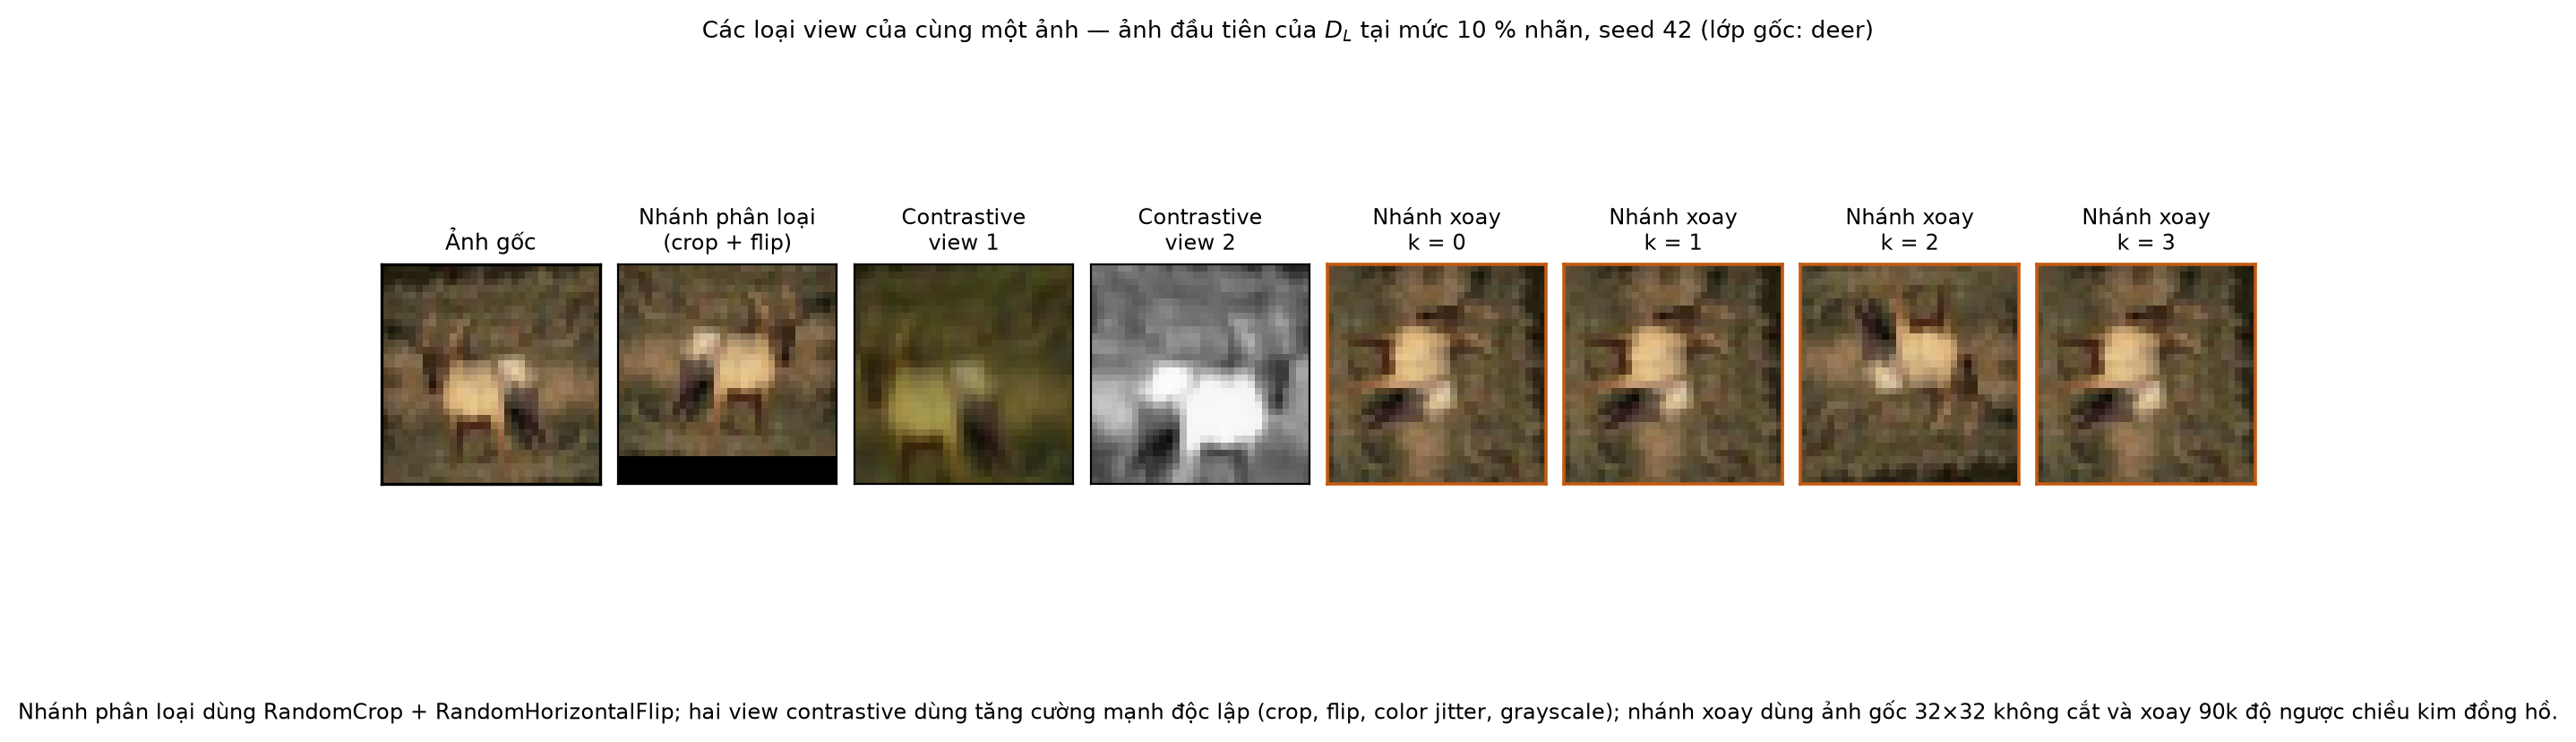
\includegraphics[width=\textwidth]{../results/figures/figA3_views.png}
  \caption{Ba loại view của cùng một ảnh (ảnh đầu tiên của $\DL$ tại mức $10\,\%$ nhãn, seed 42):
  ảnh gốc; view của nhánh phân loại; hai view của nhánh contrastive; và bốn phép xoay $k = 0..3$
  của nhánh phụ. Lưu ý nhánh xoay dùng ảnh \emph{nguyên bản} $32 \times 32$ chứ không dùng ảnh
  đã cắt.}
  \label{fig:views}
\end{figure}

\paragraph{Hằng số chuẩn hóa.}
$\text{mean} = \text{std} = (0{,}5;\ 0{,}5;\ 0{,}5)$. Đây là hằng số được chọn trước, áp dụng
chung cho mọi cấu hình và mọi mức nhãn; giá trị này \emph{không} được ước lượng từ validation
hay test, vì làm như vậy sẽ tạo rò rỉ thông tin giữa các tập.

\begin{figure}[htbp]
  \centering
  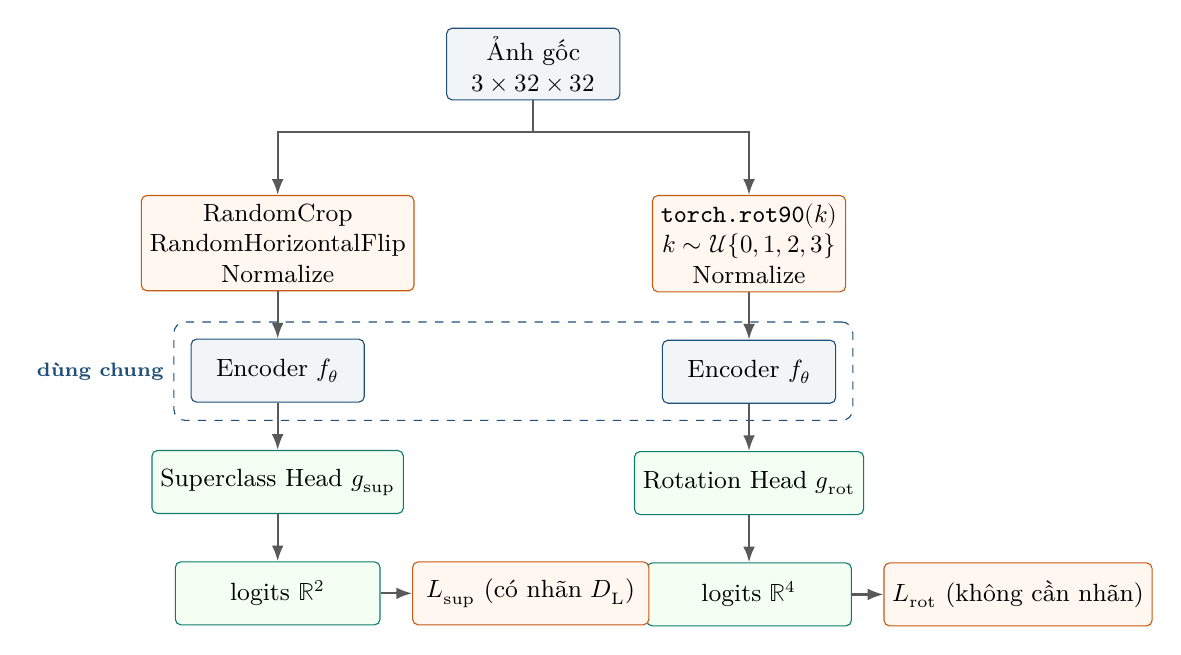
\begin{tikzpicture}[
      font=\small,
      box/.style={draw=m8blue,fill=m8light,rounded corners=2pt,minimum height=8mm,
                  minimum width=22mm,align=center,inner sep=3pt},
      sbox/.style={draw=m8teal,fill=green!5,rounded corners=2pt,minimum height=8mm,
                   minimum width=26mm,align=center,inner sep=3pt},
      abox/.style={draw=m8orange,fill=orange!6,rounded corners=2pt,minimum height=8mm,
                   align=center,inner sep=3pt},
      ar/.style={-{Latex[length=2mm]},draw=m8gray,thick},
    ]
    \node[box] (img) {Ảnh gốc\\$3\times32\times32$};

    \node[abox,below left=12mm and 4mm of img] (aug) {RandomCrop\\RandomHorizontalFlip\\Normalize};
    \node[box,below=6mm of aug] (enc1) {Encoder $\enc$};
    \node[sbox,below=6mm of enc1] (sup) {Superclass Head $\gsup$};
    \node[sbox,below=6mm of sup] (out1) {logits $\mathbb{R}^2$};

    \node[abox,below right=12mm and 4mm of img] (rot) {\code{torch.rot90}$(k)$\\$k\sim\mathcal{U}\{0,1,2,3\}$\\Normalize};
    \node[box,below=6mm of rot] (enc2) {Encoder $\enc$};
    \node[sbox,below=6mm of enc2] (head2) {Rotation Head $\grot$};
    \node[sbox,below=6mm of head2] (out2) {logits $\mathbb{R}^4$};

    \draw[ar] (img.south) -- ++(0,-4mm) -| (aug.north);
    \draw[ar] (img.south) -- ++(0,-4mm) -| (rot.north);
    \draw[ar] (aug) -- (enc1);
    \draw[ar] (enc1) -- (sup);
    \draw[ar] (sup) -- (out1);
    \draw[ar] (rot) -- (enc2);
    \draw[ar] (enc2) -- (head2);
    \draw[ar] (head2) -- (out2);

    \begin{scope}[on background layer]
      \node[draw=m8blue,dashed,rounded corners=4pt,fit=(enc1)(enc2),
            inner sep=6pt,label={[m8blue,font=\scriptsize\bfseries]left:{dùng chung}}] {};
    \end{scope}

    \node[abox,right=4mm of out1,minimum width=30mm] (l1) {$\Lsup$ (có nhãn $\DL$)};
    \node[abox,right=4mm of out2,minimum width=30mm] (l2) {$\Lrot$ (không cần nhãn)};
    \draw[ar] (out1) -- (l1);
    \draw[ar] (out2) -- (l2);
  \end{tikzpicture}
  \caption{Luồng huấn luyện hai nhánh của khối chính. Hai nhánh nhận \emph{các view khác nhau}:
  nhánh trên dùng augmentation ngẫu nhiên của ảnh chuẩn, nhánh dưới dùng ảnh đã xoay $90k$ độ.
  Encoder và các lớp BatchNorm được dùng chung, nên thống kê chạy của mạng phụ thuộc vào việc
  có nhánh xoay hay không. Các cấu hình mở rộng \cfg{E3}--\cfg{E6} thêm một nhánh thứ ba đi qua
  cùng encoder rồi qua Projection Head (\secref{sec:contrastive}); ba loại view tương ứng được
  minh họa ở \figref{fig:views}.}
  \label{fig:pipeline}
\end{figure}

% =====================================================================
\section{Phương pháp đề xuất}
\label{sec:method}
% =====================================================================

\subsection{Kiến trúc học đa nhiệm}
\label{sec:arch}

Backbone là ResNet-18 \textbf{khởi tạo ngẫu nhiên}, không dùng trọng số tiền huấn luyện. Việc
không dùng tiền huấn luyện là lựa chọn có chủ đích: nếu encoder đã được huấn luyện trước trên
ImageNet, hiệu ứng của nhiệm vụ phụ sẽ bị trộn lẫn với chất lượng đặc trưng sẵn có và không
còn đo được đóng góp của tín hiệu tự giám sát~\cite{he2016resnet,pytorch_resnet}.

Điều chỉnh cho ảnh $32 \times 32$:
\begin{itemize}[leftmargin=1.2cm,itemsep=2pt]
  \item thay convolution đầu bằng \code{Conv2d(3, 64, kernel\_size=3, stride=1, padding=1, bias=False)};
  \item bỏ lớp MaxPool đầu mạng, vì sau hai lần giảm độ phân giải $32 \to 8$ thì thông tin
        không gian còn quá ít;
  \item giữ bốn nhóm residual block, mỗi nhóm hai BasicBlock (cấu hình ResNet-18 chuẩn).
\end{itemize}

% Sinh tự động — scripts/make_report_data.py
\begin{table}[htbp]
  \centering
  \small
  \begin{tabular}{@{}l l@{}}
    \toprule
    Thành phần & Kích thước đầu ra $C \times H \times W$ \\
    \midrule
    Ảnh đầu vào & $3 \times 32 \times 32$ \\
    Conv $3\times3$ + BatchNorm + ReLU & $64 \times 32 \times 32$ \\
    Nhóm residual 1: 2 BasicBlock & $64 \times 32 \times 32$ \\
    Nhóm residual 2: 2 BasicBlock & $128 \times 16 \times 16$ \\
    Nhóm residual 3: 2 BasicBlock & $256 \times 8 \times 8$ \\
    Nhóm residual 4: 2 BasicBlock & $512 \times 4 \times 4$ \\
    Global Average Pooling + Flatten & vector 512 chiều \\
    Superclass Head (tuyến tính, có bias) & $512 \to 2$ \\
    Rotation Head (tuyến tính, có bias) & $512 \to 4$ \\
    \bottomrule
  \end{tabular}
  \caption{Chuỗi kích thước tensor của backbone ResNet-18 điều chỉnh cho ảnh $32 \times 32$. Các giá trị này được kiểm tra tự động bằng \texttt{scripts/self\_test.py} trên môi trường thực nghiệm.}
  \label{tab:arch}
\end{table}

\paragraph{Ký hiệu.}
$\enc$ là encoder dùng chung; $\gsup$ và $\grot$ là hai head tương ứng; $\norm$ là bước chuyển
tensor và chuẩn hóa; $R_k$ là phép xoay $90k$ độ. Hai đầu ra được viết:

\begin{align}
  a_{\mathrm{sup}} &= \gsup\bigl(\enc(t_{\mathrm{sup}}(x))\bigr) \in \mathbb{R}^2, \label{eq:asup}\\
  a_{\mathrm{rot}} &= \grot\bigl(\enc(\norm(R_k(x)))\bigr) \in \mathbb{R}^4, \label{eq:arot}
\end{align}

trong đó $t_{\mathrm{sup}}(\cdot)$ là chuỗi augmentation của nhánh phân loại. Việc viết tách
$t_{\mathrm{sup}}$ và $\norm \circ R_k$ nhấn mạnh rằng \textbf{hai nhánh nhận các view khác
nhau}; ta không giả định tồn tại một vector đặc trưng duy nhất dùng cho cả ảnh chuẩn và ảnh đã
xoay.

\paragraph{Cách ghép minibatch.}
Khi huấn luyện M8, hai minibatch được ghép theo chiều batch trước khi qua encoder:
$[\,B_L;\, B_R\,] \in \mathbb{R}^{(b_L + b_R) \times 3 \times 32 \times 32}$, sau đó tách đặc
trưng trở lại đúng head. \textbf{Các lớp BatchNorm dùng chung}, do đó mọi thay đổi về thành phần
của batch đều làm thay đổi thống kê chạy của toàn mạng~\cite{ioffe2015batchnorm}. Đây là cơ sở
cho một giới hạn quan trọng được nêu ở \secref{sec:exp-compare}: không thể diễn giải so sánh
\cfg{E2-L}/\cfg{E1} như một phép tách hoàn toàn riêng tác dụng của nhãn góc xoay khỏi mọi thay
đổi về mặt tính toán.

\paragraph{Suy luận.}
Khi suy luận, chỉ chạy encoder và Superclass Head; chọn lớp bằng $\arg\max$ của hai logits.
Rotation Head không cần thiết và không được tính vào chi phí suy luận. Hệ quả kiến trúc: mô
hình suy luận của \cfg{E2} có \emph{đúng cùng} kiến trúc với \cfg{E1}, nên không thể kỳ vọng
giảm độ phức tạp kiến trúc chỉ nhờ bỏ head phụ.

\subsection{Hàm mất mát và cách sử dụng dữ liệu}
\label{sec:loss}

Với $B_L$ là minibatch có nhãn, $B_R$ là minibatch cho nhiệm vụ xoay, và $b_L$, $b_R$ là số mẫu
tương ứng, hai mất mát được lấy \textbf{trung bình riêng}:

\begin{align}
  \Lsup &= \frac{1}{b_L}\sum_{i=1}^{b_L} \mathrm{CE}\bigl(a_{\mathrm{sup},i},\, y_i\bigr),
  \label{eq:lsup}\\
  \Lrot &= \frac{1}{b_R}\sum_{j=1}^{b_R} \mathrm{CE}\bigl(a_{\mathrm{rot},j},\, k_j\bigr),
  \label{eq:lrot}\\
  L &= \Lsup + \lamrot \Lrot. \label{eq:total}
\end{align}

$\mathrm{CE}$ là cross-entropy cho nhãn lớp nguyên. Trong PyTorch, logits được truyền trực tiếp
vào \code{CrossEntropyLoss}, \textbf{không} áp dụng Softmax trước loss; việc áp Softmax hai lần
là một lỗi phổ biến làm hỏng gradient~\cite{pytorch_ce}. Trong mã nguồn, logits được truyền
nguyên vẹn vào lớp này.

\paragraph{Phân chia nguồn dữ liệu cho từng mất mát.}
Chỉ ảnh thuộc $\DL$ đóng góp vào $\Lsup$. Ngược lại, $B_R$ lấy từ $\DL$ hoặc từ $\Dtrain$ tùy
cấu hình (\tabref{tab:configs}). Chốt $\lamrot = 0{,}5$ cho thí nghiệm chính; các giá trị khác
chỉ thuộc khảo sát độ nhạy đã khai báo trước.

\begin{keybox}
\textbf{Vì sao lấy trung bình riêng từng mất mát?} Nếu gộp hai tập mẫu rồi lấy trung bình chung,
trọng số hiệu dụng của nhánh xoay sẽ phụ thuộc vào tỷ lệ $b_R/b_L$, và như vậy $\lamrot$ mất ý
nghĩa so sánh giữa các mức nhãn. Lấy trung bình riêng giữ cho $\lamrot$ là một hệ số có thể
diễn giải được và giữ phép so sánh độ nhạy $\lamrot$ nhất quán.
\end{keybox}

\subsection{Mở rộng Contrastive Learning và SupCon}
\label{sec:contrastive}

Nội dung này là \textbf{hướng mở rộng} của đề tài: nó không phải điều kiện hoàn thành phần
chính và được chạy \emph{sau} khi khối đối chứng \cfg{E1}/\cfg{E2-L}/\cfg{E2} đã hoàn tất.
Bốn cấu hình \cfg{E3}--\cfg{E6} được triển khai và báo cáo tại \secref{sec:results-ext}.

\paragraph{Contrastive Learning tự giám sát (NT-Xent).}
Tạo hai view của cùng một ảnh và đưa qua encoder cùng Projection Head; hai view này tạo thành
positive pair. Có thể dùng ảnh từ $\Dtrain$ vì \textbf{không} cần nhãn siêu lớp. Theo tham chiếu
SimCLR~\cite{chen2020simclr}, mọi thành phần đều được khóa trước: loss NT-Xent, chuẩn hóa vector
$L_2$, nhiệt độ $\tau_{\mathrm{NT}}$, phép tăng cường ảnh, kích thước batch và chiều Projection
Head. Với $2N$ view trong một minibatch và $j(i)$ là view còn lại của cùng ảnh:

\begin{equation}
  L_{\mathrm{NT\text{-}Xent}}
  = \frac{1}{2N}\sum_{i=1}^{2N} -\log
    \frac{\exp\!\bigl(s_{i,j(i)}/\tau_{\mathrm{NT}}\bigr)}
         {\sum_{k \neq i} \exp\!\bigl(s_{i,k}/\tau_{\mathrm{NT}}\bigr)},
  \qquad
  s_{i,k} = \frac{z_i^{\top} z_k}{\lVert z_i\rVert_2 \lVert z_k\rVert_2}.
  \label{eq:ntxent}
\end{equation}

\paragraph{Supervised Contrastive Learning (SupCon).}
Xây dựng positive pair từ \textbf{các view có cùng nhãn siêu lớp đã được cấp cho huấn luyện}.
Trong đề tài này, SupCon chỉ sử dụng $\DL$; \textbf{không} đọc nhãn thật của $\DU$. SupCon là
học \emph{có} giám sát, không được gọi là một nhiệm vụ tự giám sát~\cite{khosla2020supcon}. Với
$A(i) = \{a \neq i : \tilde{y}_a = \tilde{y}_i\}$ là tập positive của view $i$:

\begin{equation}
  L_{\mathrm{SupCon}}
  = \sum_{i=1}^{2N} \frac{-1}{|A(i)|}
    \sum_{a \in A(i)} \log
    \frac{\exp\!\bigl(s_{i,a}/\tau_{\mathrm{Sup}}\bigr)}
         {\sum_{k \neq i} \exp\!\bigl(s_{i,k}/\tau_{\mathrm{Sup}}\bigr)}.
  \label{eq:supcon}
\end{equation}

\paragraph{Kiến trúc Projection Head.}
Hai lớp tuyến tính $512 \to 512 \to \dim_{\mathrm{proj}}$ với BatchNorm và ReLU ở lớp ẩn
(theo SupCon/SimCLR). Head này \textbf{chỉ} tồn tại khi huấn luyện; khi suy luận, mô hình chỉ
gồm encoder và Superclass Head, nên \emph{số tham số suy luận không thay đổi} so với
\cfg{E1}/\cfg{E2} (xem \tabref{tab:inference-cost} và \tabref{tab:extension-cost}).

\subsection{Đối chứng bắt buộc}
\label{sec:baselines}

Ba cấu hình chính được thiết kế để tách bạch hai yếu tố thường bị trộn lẫn: \emph{việc thêm
nhiệm vụ phụ} và \emph{việc mở rộng nguồn ảnh cho nhiệm vụ phụ}.

% Sinh tự động — scripts/make_report_data.py
\begin{table}[htbp]
  \centering
  \small
  \begin{tabular}{@{}l l l l@{}}
    \toprule
    ID & Cấu hình & Ảnh cho phân loại & Ảnh cho nhiệm vụ xoay \\
    \midrule
    \cfg{E1}   & Baseline chỉ học siêu lớp & $\DL$ & Không có \\
    \cfg{E2-L} & Thêm nhánh xoay, cùng tập nguồn & $\DL$ & Chỉ $\DL$ \\
    \cfg{E2}   & Thêm nhánh xoay, mở rộng nguồn ảnh & $\DL$ & $\Dtrain = \DL \cup \DU$ \\
    \bottomrule
  \end{tabular}
  \caption{Ba cấu hình chính. \cfg{E1} và \cfg{E2} là cặp đối chứng chính; \cfg{E2-L} tách riêng tác dụng của việc mở rộng nguồn ảnh cho nhánh phụ.}
  \label{tab:configs}
\end{table}

% Sinh tự động — scripts/make_report_data.py
\begin{table}[htbp]
  \centering
  \footnotesize
  \setlength{\tabcolsep}{4pt}
  \begin{tabular}{@{}l l l l@{}}
    \toprule
    ID & Hàm mục tiêu & Nguồn ảnh cho xoay & Nguồn ảnh cho loss bổ sung \\
    \midrule
    \cfg{E3} & $\Lsup + \lamc \Lntxent$ & Không có nhánh xoay & $\Dtrain$; không dùng nhãn siêu lớp \\
    \cfg{E4} & $\Lsup + \lamc \Lsupcon$ & Không có nhánh xoay & Chỉ $\DL$ có nhãn hợp lệ \\
    \cfg{E5} & $\Lsup + \lamrot \Lrot + \lamc \Lntxent$ & $\Dtrain$ & NT-Xent: $\Dtrain$; rotation: $\Dtrain$ \\
    \cfg{E6} & $\Lsup + \lamrot \Lrot + \lamc \Lsupcon$ & $\Dtrain$ & SupCon: $\DL$; rotation: $\Dtrain$ \\
    \bottomrule
  \end{tabular}
  \caption{Bốn cấu hình mở rộng contrastive. $\lamc$ dùng chung cho mọi cấu hình và được khóa bằng validation trước khi đánh giá test (\secref{sec:results-ext-lambda}). SupCon chỉ dùng $\DL$; NT-Xent dùng $\Dtrain$ vì không cần nhãn siêu lớp.}
  \label{tab:extensions}
\end{table}

Ba so sánh ghép cặp được dùng để trả lời các câu hỏi đã nêu:

\begin{itemize}[leftmargin=1.2cm,itemsep=3pt]
  \item \textbf{\cfg{E2-L} so với \cfg{E1}:} tác động của việc bổ sung nhánh rotation khi
        \emph{không} mở rộng tập ảnh nguồn. Đây là phép so sánh cô lập nhất về mặt dữ liệu,
        nhưng vẫn còn khác biệt về tính toán.
  \item \textbf{\cfg{E2} so với \cfg{E2-L}:} ảnh hưởng của việc mở rộng nguồn ảnh cho nhánh phụ
        (chỉ $\DL$ so với toàn bộ $\Dtrain$). Hai cấu hình này có cùng hàm mục tiêu và cùng số
        bước cập nhật, chỉ khác nguồn ảnh của $B_R$.
  \item \textbf{\cfg{E2} so với \cfg{E1}:} hiệu quả tổng thể của M8 trong cùng ngân sách nhãn;
        đây là so sánh trả lời trực tiếp câu hỏi C1.
\end{itemize}

Các so sánh được ghép cặp theo lần lặp và tỷ lệ nhãn, tức $\Delta_s = \mathrm{Macro\text{-}F1}_s(\text{M8}) -
\mathrm{Macro\text{-}F1}_s(\cfg{E1})$ tính riêng cho từng $s$ rồi mới tổng hợp.

\begin{warnbox}
\textbf{Giới hạn về tính công bằng của phép so sánh.} \cfg{E2-L}/\cfg{E2} vẫn xử lý thêm view và
làm thay đổi thống kê BatchNorm so với \cfg{E1}. Do đó \textbf{không} diễn giải chúng là phép
tách hoàn toàn riêng tác dụng của \enquote{nhãn góc xoay} khỏi mọi thay đổi về tính toán.
Tương tự, \textbf{không} khẳng định so sánh công bằng về FLOPs hoặc thời gian chỉ vì ba cấu hình
dùng cùng số epoch: số lượt ảnh được xử lý ở mỗi bước cập nhật là khác nhau.
\end{warnbox}

% =====================================================================
\section{Thiết kế thực nghiệm và chỉ số}
\label{sec:experiments}
% =====================================================================

\subsection{Môi trường thực nghiệm}
\label{sec:env}

Toàn bộ thí nghiệm được chạy trong một môi trường ảo Python tách biệt nhằm bảo đảm khả năng
tái lập. Thông tin môi trường dưới đây được đọc trực tiếp từ chính phiên bản phần mềm đã dùng
để huấn luyện và đo thời gian, không suy ra từ phiên bản của trang tài liệu.

\begin{table}[htbp]
  \centering
  \small
  \begin{tabular}{@{}l l@{}}
    \toprule
    Thành phần & Giá trị thực tế \\
    \midrule
    Python & \REnvPython \\
    PyTorch & \REnvTorch \\
    TorchVision & \REnvTorchvision \\
    Bản dựng CUDA & \REnvCudaBuild \\
    GPU & \REnvGpu \\
    VRAM & \REnvVram{} GiB \\
    CPU & \REnvCpu \\
    Số luồng CPU & \REnvCores \\
    RAM & \REnvRam{} GiB \\
    \bottomrule
  \end{tabular}
  \caption{Môi trường thực nghiệm được ghi lại tự động vào \code{results/environment.json} và
  \code{results/self\_test.json}. Số luồng CPU được ghim bằng \code{torch.set\_num\_threads}
  trước các phép đo độ trễ.}
  \label{tab:env}
\end{table}

\paragraph{Tạo môi trường.}
\begin{lstlisting}[language=bash,caption={Cài đặt môi trường ảo và các gói phụ thuộc.},label={lst:setup}]
python -m venv .venv
.venv\Scripts\python.exe -m pip install --upgrade pip
.venv\Scripts\python.exe -m pip install --index-url https://download.pytorch.org/whl/cu128 `
    torch==2.11.0 torchvision==0.26.0
.venv\Scripts\python.exe -m pip install -r requirements.txt
\end{lstlisting}

\subsection{Cấu hình huấn luyện}
\label{sec:train-config}

Để thống nhất số bước cập nhật có giám sát giữa các cấu hình, bảng kết quả chính
\textbf{không dùng Early Stopping}. Cả ba cấu hình chạy đúng 100 epoch và đều được phép chọn
checkpoint bằng cùng một tiêu chí validation. Early Stopping với \code{patience=10} của bản
đề cương ban đầu chỉ có thể dùng cho các thử nghiệm thăm dò và phải được ghi rõ; nó
\textbf{không} được trộn vào bảng so sánh chính vì sẽ tạo ra số epoch khác nhau giữa các cấu
hình.

% Sinh tự động — scripts/make_report_data.py
\begin{table}[htbp]
  \centering
  \small
  \begin{tabular}{@{}l l@{}}
    \toprule
    Thành phần & Thiết lập cho thí nghiệm chính \\
    \midrule
    Optimizer & AdamW \\
    Learning rate & $3 \times 10^{-4}$ \\
    Weight decay & $10^{-4}$ \\
    Betas & $(0{,}9;\ 0{,}999)$ \\
    Eps & $10^{-8}$ \\
    Kích thước minibatch $B_L$ & tối đa 128 ảnh \\
    Kích thước minibatch $B_R$ & bằng $B_L$ tại mỗi bước \\
    Ngân sách học & 100 epoch ($1$ epoch $=$ một lượt duyệt $\DL$) \\
    Scheduler & CosineAnnealingLR, $T_{\max}=100$, $\eta_{\min}=0$ \\
    Hệ số $\lamrot$ & $0{,}5$ cho thí nghiệm chính \\
    Chọn checkpoint & Macro-F1 validation cao nhất; hòa thì loss thấp hơn, rồi epoch sớm hơn \\
    Early stopping & Không dùng trong bảng kết quả chính \\
    Seed & chia split 2026; lần lặp 42, 43, 44 \\
    Chuẩn hóa & mean $=$ std $= (0{,}5;\ 0{,}5;\ 0{,}5)$ \\
    \bottomrule
  \end{tabular}
  \caption{Cấu hình huấn luyện dùng chung cho cả ba cấu hình. Ba cấu hình ghép cặp dùng cùng trọng số khởi tạo của encoder và Superclass Head.}
  \label{tab:hyperparams}
\end{table}

\paragraph{Một epoch được định nghĩa thế nào.}
Một epoch là \emph{một lượt duyệt toàn bộ $\DL$}, không phải một lượt duyệt $\Dtrain$. Nhờ định
nghĩa này, ba mức nhãn có số epoch giống nhau và số bước cập nhật có giám sát tỷ lệ với
$|\DL|$. Minibatch cuối nhỏ hơn 128 được \emph{giữ lại} chứ không bỏ mẫu, nên không có ảnh nào
bị loại khỏi huấn luyện.

\paragraph{Chọn checkpoint.} Tiêu chí là Macro-F1 validation cao nhất. Khi hai epoch có cùng
Macro-F1 (trong sai số $10^{-12}$), ưu tiên loss phân loại validation thấp hơn; nếu vẫn bằng
nhau, chọn epoch sớm hơn. Tập test không tham gia vào bước này dưới bất kỳ hình thức nào.

\subsection{Quy trình và nguyên tắc so sánh}
\label{sec:exp-compare}

Trong mỗi epoch, duyệt $\DL$ một lần với \emph{cùng chuỗi minibatch có giám sát} cho các cấu
hình ghép cặp: cùng seed cho \code{DataLoader}, cùng thứ tự mẫu, cùng phép augmentation. Với mỗi
bước của M8, lấy $B_R$ ngẫu nhiên từ nguồn ảnh quy định tại \tabref{tab:configs}; dùng một bộ
sinh số ngẫu nhiên \textbf{độc lập} để việc lấy ảnh và góc xoay không làm thay đổi augmentation
của nhánh phân loại. Sau đó tính tổng loss và thực hiện một bước optimizer.

\begin{keybox}
\textbf{Vì sao cần bộ sinh số ngẫu nhiên độc lập?} Nếu nhánh phụ dùng chung luồng RNG với nhánh
chính, việc thêm nhánh phụ sẽ \emph{dịch chuyển} chuỗi số ngẫu nhiên của nhánh chính. Khi đó
hai cấu hình ghép cặp sẽ thấy các phép augmentation khác nhau, và chênh lệch $\Delta_s$ trở
thành nhiễu ngẫu nhiên thay vì tín hiệu cần đo.
\end{keybox}

\paragraph{\cfg{E1} không chạy nhánh rotation, kể cả forward.}
Đặt $\lamrot = 0$ nhưng vẫn đưa ảnh xoay qua BatchNorm \textbf{không} được xem là baseline
\cfg{E1}, vì thống kê chạy của mạng vẫn có thể bị thay đổi: các lớp BatchNorm cập nhật
running mean và running variance ngay cả khi gradient của nhánh đó bị nhân với $0$. Trong mã
nguồn, \cfg{E1} được khởi tạo \emph{không có} Rotation Head và vòng huấn luyện bỏ hoàn toàn
nhánh phụ.

\paragraph{Không dùng nhãn của $\DU$.}
Với mọi cấu hình, nhãn của $\DU$ không được dùng để phân tầng minibatch huấn luyện, không được
dùng để xây dựng mục tiêu học, và không được dùng cho bất kỳ quyết định thiết kế nào.

\paragraph{Quy mô khối thực nghiệm.}
Khối chính gồm $3 \text{ cấu hình} \times 3 \text{ mức nhãn} \times 3 \text{ lần lặp} =
\RRuns$ lượt huấn luyện. Ba lần lặp thay đổi \emph{cả} tập con có nhãn \emph{lẫn} ngẫu nhiên
huấn luyện (khởi tạo, thứ tự dữ liệu, augmentation), trong khi phép chia
train/validation/test được cố định. Đây \textbf{không} phải cross-validation: cùng một tập
validation được dùng cho mọi lần lặp, nên ba lần lặp chỉ đo độ ổn định trước hai nguồn ngẫu
nhiên chứ không ước lượng được phương sai do chính phép chia dữ liệu gây ra.

\paragraph{Khảo sát tùy chọn.} $\lamrot \in \{0{,}1;\ 0{,}25;\ 0{,}5;\ 1{,}0\}$ tại mức
$10\,\%$ nhãn, được ưu tiên trước các mở rộng E3--E6. Giữ $\lamrot = 0{,}5$ cho so sánh chính.
Không được lựa chọn $\lam$ hay cấu hình dựa trên kết quả test. Nếu tài nguyên không đủ, phải
điều chỉnh ngân sách chung và ghi nhận \emph{trước khi} mở kết quả test.

\paragraph{Quy trình khóa siêu tham số của phần mở rộng.}
Khối mở rộng contrastive \cfg{E3}--\cfg{E6} có thêm ba siêu tham số phải khóa trước khi đánh giá
test: nhiệt độ SupCon ($0{,}1$), nhiệt độ NT-Xent ($0{,}2$) và hệ số $\lamc$. Hai nhiệt độ và
chiều Projection Head ($128$) được chốt theo giá trị chuẩn của tài liệu
gốc~\cite{chen2020simclr,khosla2020supcon}; riêng $\lamc$ được chọn bằng \textbf{Macro-F1
validation} qua một script \emph{không có} bước đánh giá test (\secref{sec:results-ext-lambda}).
Quy tắc chọn được khai báo trước khi chạy để tránh điều chỉnh giao thức sau khi đã thấy kết quả.

\subsection{Chỉ số và cách báo cáo}
\label{sec:metrics}

Chỉ số chính là \textbf{Macro-F1} của Animal và Vehicle. Báo cáo thêm Accuracy,
precision/recall/F1 từng lớp và ma trận nhầm lẫn trên toàn bộ 10.000 ảnh test. Mỗi ảnh chỉ nhận
một dự đoán của nhánh siêu lớp; \textbf{không} dùng test-time augmentation trong thí nghiệm
chính.

Các chỉ số được định nghĩa như sau:

\begin{align}
  \mathrm{Accuracy} &= \frac{1}{N}\sum_{i=1}^{N} \mathbb{1}\!\left[\hat{y}_i = y_i\right],
  \label{eq:acc}\\
  P_c &= \frac{\mathrm{TP}_c}{\mathrm{TP}_c + \mathrm{FP}_c}, \qquad
  R_c = \frac{\mathrm{TP}_c}{\mathrm{TP}_c + \mathrm{FN}_c}, \label{eq:pr}\\
  \mathrm{F1}_c &= \frac{2 P_c R_c}{P_c + R_c}, \qquad
  \mathrm{Macro\text{-}F1} = \frac{\mathrm{F1}_{\mathrm{Animal}} + \mathrm{F1}_{\mathrm{Vehicle}}}{2}.
  \label{eq:macro}
\end{align}

\paragraph{Quy ước biên.} Nếu mẫu số của precision, recall hoặc F1 bằng $0$, giá trị tương ứng
được quy ước bằng $0$ và dùng thống nhất cho mọi cấu hình. Chỉ số được tính từ \emph{toàn bộ}
dự đoán của tập đánh giá; không lấy trung bình không trọng số các F1 của từng minibatch, vì
làm như vậy sẽ cho trọng số sai cho các minibatch nhỏ ở cuối epoch.

\paragraph{Cách tổng hợp.} Báo cáo trung bình $\pm$ độ lệch chuẩn mẫu qua ba lần lặp và chênh
lệch ghép cặp $\Delta_s = \mathrm{Macro\text{-}F1}_s(\text{M8}) -
\mathrm{Macro\text{-}F1}_s(\cfg{E1})$ tính bằng điểm phần trăm. Mức $10\,\%$ là so sánh ưu
tiên; mức $20\,\%$ và $50\,\%$ dùng để đánh giá xu hướng.

\begin{warnbox}
\textbf{Giới hạn suy luận thống kê.} Ba lần lặp chỉ cho bằng chứng ban đầu về độ ổn định.
Với $n=3$ và độ lệch chuẩn quan sát được, khoảng tin cậy rất rộng và không có cơ sở để tuyên
bố \enquote{có ý nghĩa thống kê} hay \enquote{luôn tốt hơn}. Đặc biệt, \textbf{không} được chọn
một lần chạy tốt nhất rồi kết luận từ nó: báo cáo dùng trung bình và độ lệch chuẩn qua cả ba
lần~\cite{bouthillier2021variance}.
\end{warnbox}

\paragraph{Rotation Accuracy.} Chỉ là chỉ số \emph{chẩn đoán} cho nhánh phụ. Nếu đo trên
validation, phải đánh giá đủ bốn phép xoay cho mỗi ảnh và ghi rõ giao thức. Độ chính xác cao ở
nhiệm vụ phụ \textbf{không} thay thế bằng chứng cải thiện Macro-F1 của nhiệm vụ chính; một
nhiệm vụ phụ được học tốt vẫn hoàn toàn có thể không giúp gì cho nhiệm vụ chính.

\subsection{Chi phí suy luận và giới hạn kết luận về IoT}
\label{sec:cost-protocol}

\paragraph{Đếm tham số và dung lượng.} Đếm riêng số tham số khi huấn luyện và khi suy luận; đo
dung lượng tệp chỉ chứa trọng số suy luận, \textbf{không} gộp optimizer state (vì optimizer
state không tồn tại trên thiết bị triển khai). Với cấu hình tại \secref{sec:arch}, mô hình suy
luận có \RParamInference{} tham số; Rotation Head thêm \RParamRotationHead{} tham số. Phần tham
số FP32 của mô hình suy luận tương đương khoảng \RParamInferenceMiB{} MiB, \emph{chưa} gồm
buffer, activation và bộ nhớ của runtime~\cite{pytorch_resnet}. Đây là thông số kiến trúc, không
phải kết quả huấn luyện.

\paragraph{Giao thức đo độ trễ.} Đo với batch $=1$, tensor $1 \times 3 \times 32 \times 32$,
FP32, \code{model.eval()} và \code{torch.inference\_mode()}. Dùng \emph{cùng} máy, cùng runtime
và cùng số luồng CPU cho mọi cấu hình. Chạy khởi động 50 lượt, sau đó đo tối thiểu 1.000 lượt
trên cùng các ảnh validation đã tiền xử lý. Nếu đo trên GPU, đồng bộ trước và sau khối tính thời
gian. Báo cáo mean, median, p95 theo ms/ảnh; lặp ba phiên và lưu log~\cite{pytorch_benchmark}.

\paragraph{Tách riêng các thành phần thời gian.} Phép đo trên chỉ tính thời gian \emph{suy luận
của mô hình}. Thời gian đọc ảnh, tiền xử lý và truyền dữ liệu phải được đo và báo cáo riêng.
Hai mô hình \cfg{E1} và \cfg{E2} có \emph{cùng} kiến trúc suy luận, nên không kỳ vọng giảm độ
phức tạp kiến trúc chỉ nhờ bỏ head phụ.

% =====================================================================
\section{Kết quả thực nghiệm}
\label{sec:results}
% =====================================================================

Trong phần này, mọi giá trị số đều được đọc trực tiếp từ các tệp
\code{results/checkpoints/*.json} do quá trình huấn luyện sinh ra. Không có giá trị nào được
nhập bằng tay.

\subsection{Khối thực nghiệm chính}
\label{sec:results-main}

Khối thực nghiệm hoàn thành \RRuns{} lượt huấn luyện ($3$ cấu hình $\times$ $3$ mức nhãn
$\times$ $3$ lần lặp), tổng thời gian huấn luyện \RTotalHours{} giờ trên
\REnvGpu{}. Chi tiết từng lượt được liệt kê ở \tabref{tab:per-run}; bảng tổng hợp kết quả trên
tập test là \tabref{tab:main-results}.

% Sinh tự động — scripts/make_report_data.py
\begin{table}[htbp]
  \centering
  \scriptsize
  \setlength{\tabcolsep}{4.5pt}
  \begin{tabular}{@{}l r r r r r r r r r@{}}
    \toprule
    \multirow{2}{*}{\makecell[l]{Cấu hình}} & \multicolumn{3}{c}{10\,\% nhãn} & \multicolumn{3}{c}{20\,\% nhãn} & \multicolumn{3}{c}{50\,\% nhãn} \\
    \cmidrule(lr){2-4}\cmidrule(lr){5-7}\cmidrule(lr){8-10}
     & Macro-F1 & Acc. & $\Delta$ & Macro-F1 & Acc. & $\Delta$ & Macro-F1 & Acc. & $\Delta$ \\

    \midrule
    \cfg{E1} & 0,9319 & 0,9349 & --- & 0,9497 & 0,9517 & --- & 0,9690 & 0,9702 & --- \\
    \cfg{E2-L} & 0,9313 & 0,9340 & $$-$0,06$ & 0,9505 & 0,9524 & $+0,08$ & 0,9745 & 0,9755 & $+0,55$ \\
    \cfg{E2} & 0,9470 & 0,9492 & $+1,51$ & 0,9631 & 0,9645 & $+1,34$ & 0,9777 & 0,9786 & $+0,88$ \\
    \bottomrule
  \end{tabular}
  \caption{Kết quả trên $\Dtest$: Macro-F1 và Accuracy (\enquote{Acc.}) là trung bình qua ba lần lặp. $\Delta$ là chênh lệch Macro-F1 trung bình so với \cfg{E1} ở cùng mức nhãn, tính bằng điểm phần trăm; giá trị dương nghĩa là cấu hình đa nhiệm tốt hơn baseline. Độ lệch chuẩn qua ba lần lặp được báo cáo ở \tabref{tab:main-std}.}
  \label{tab:main-results}
\end{table}

% Sinh tự động — scripts/make_report_data.py
\begin{table}[htbp]
  \centering
  \small
  \setlength{\tabcolsep}{5pt}
  \begin{tabular}{@{}l c c c@{}}
    \toprule
    Cấu hình & 10\,\% nhãn & 20\,\% nhãn & 50\,\% nhãn \\
    \midrule
    \cfg{E1} & $0,9319 \pm 0,0035$ & $0,9497 \pm 0,0030$ & $0,9690 \pm 0,0015$ \\
    \cfg{E2-L} & $0,9313 \pm 0,0030$ & $0,9505 \pm 0,0027$ & $0,9745 \pm 0,0017$ \\
    \cfg{E2} & $0,9470 \pm 0,0034$ & $0,9631 \pm 0,0047$ & $0,9777 \pm 0,0022$ \\
    \bottomrule
  \end{tabular}
  \caption{Macro-F1 trên $\Dtest$ dạng trung bình $\pm$ độ lệch chuẩn mẫu qua ba lần lặp. Ba lần lặp chỉ cung cấp bằng chứng ban đầu về độ ổn định, không đủ để kết luận về ý nghĩa thống kê.}
  \label{tab:main-std}
\end{table}

\begin{figure}[htbp]
  \centering
  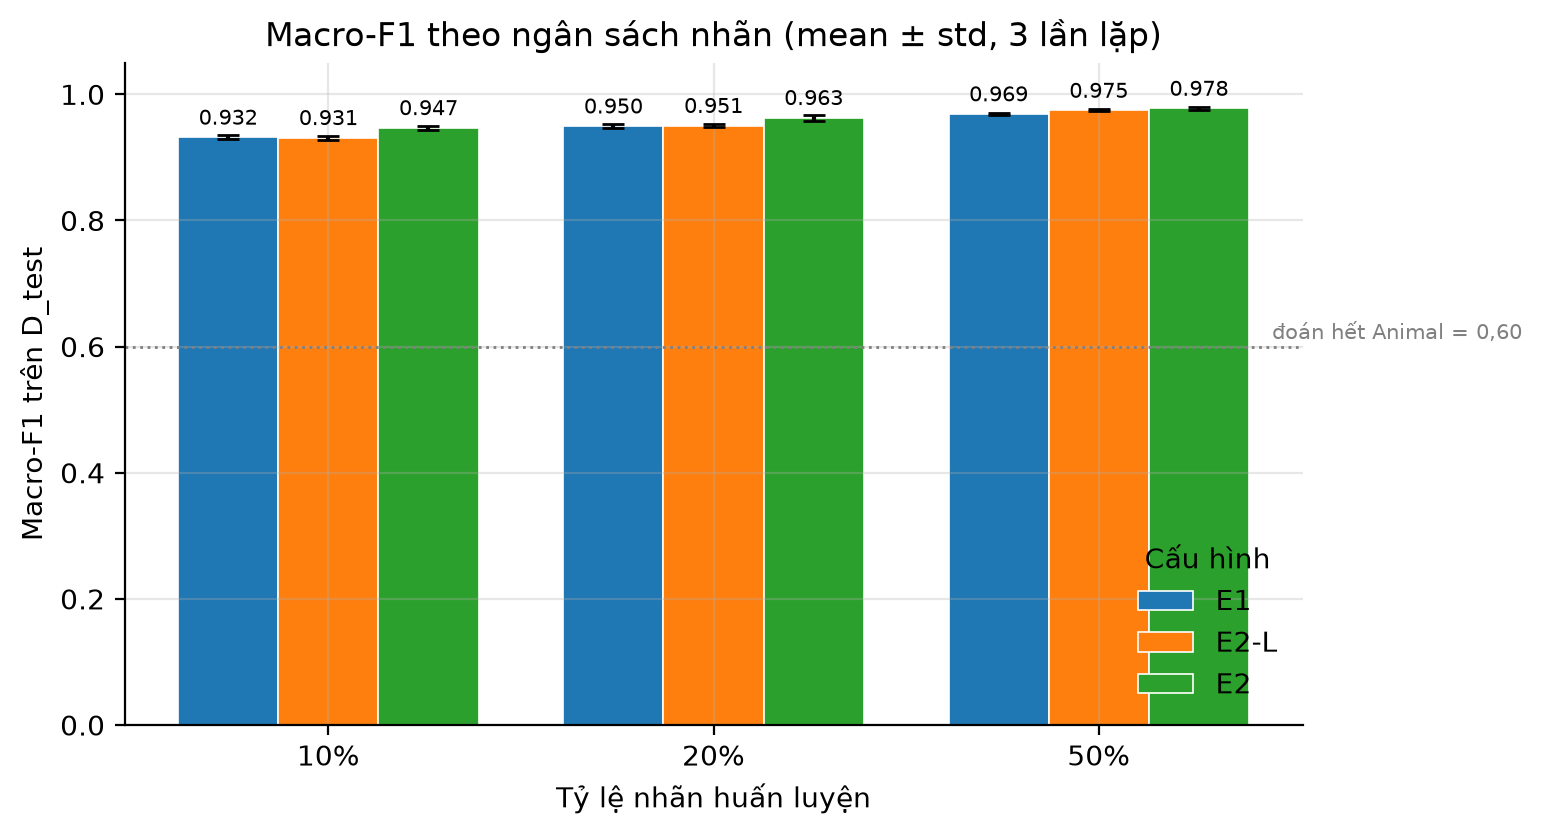
\includegraphics[width=\textwidth]{../results/figures/fig02_macro_f1_by_budget.png}
  \caption{Macro-F1 trên $\Dtest$ theo ngân sách nhãn cho ba cấu hình. Cột là trung bình qua ba
  lần lặp, thanh sai số là một độ lệch chuẩn mẫu. Đường chấm ngang ở $0{,}60$ đánh dấu mức
  Accuracy của bộ phân loại luôn đoán \enquote{Animal}; mọi cấu hình đều vượt mức này rõ rệt.}
  \label{fig:macro-f1}
\end{figure}

\begin{figure}[htbp]
  \centering
  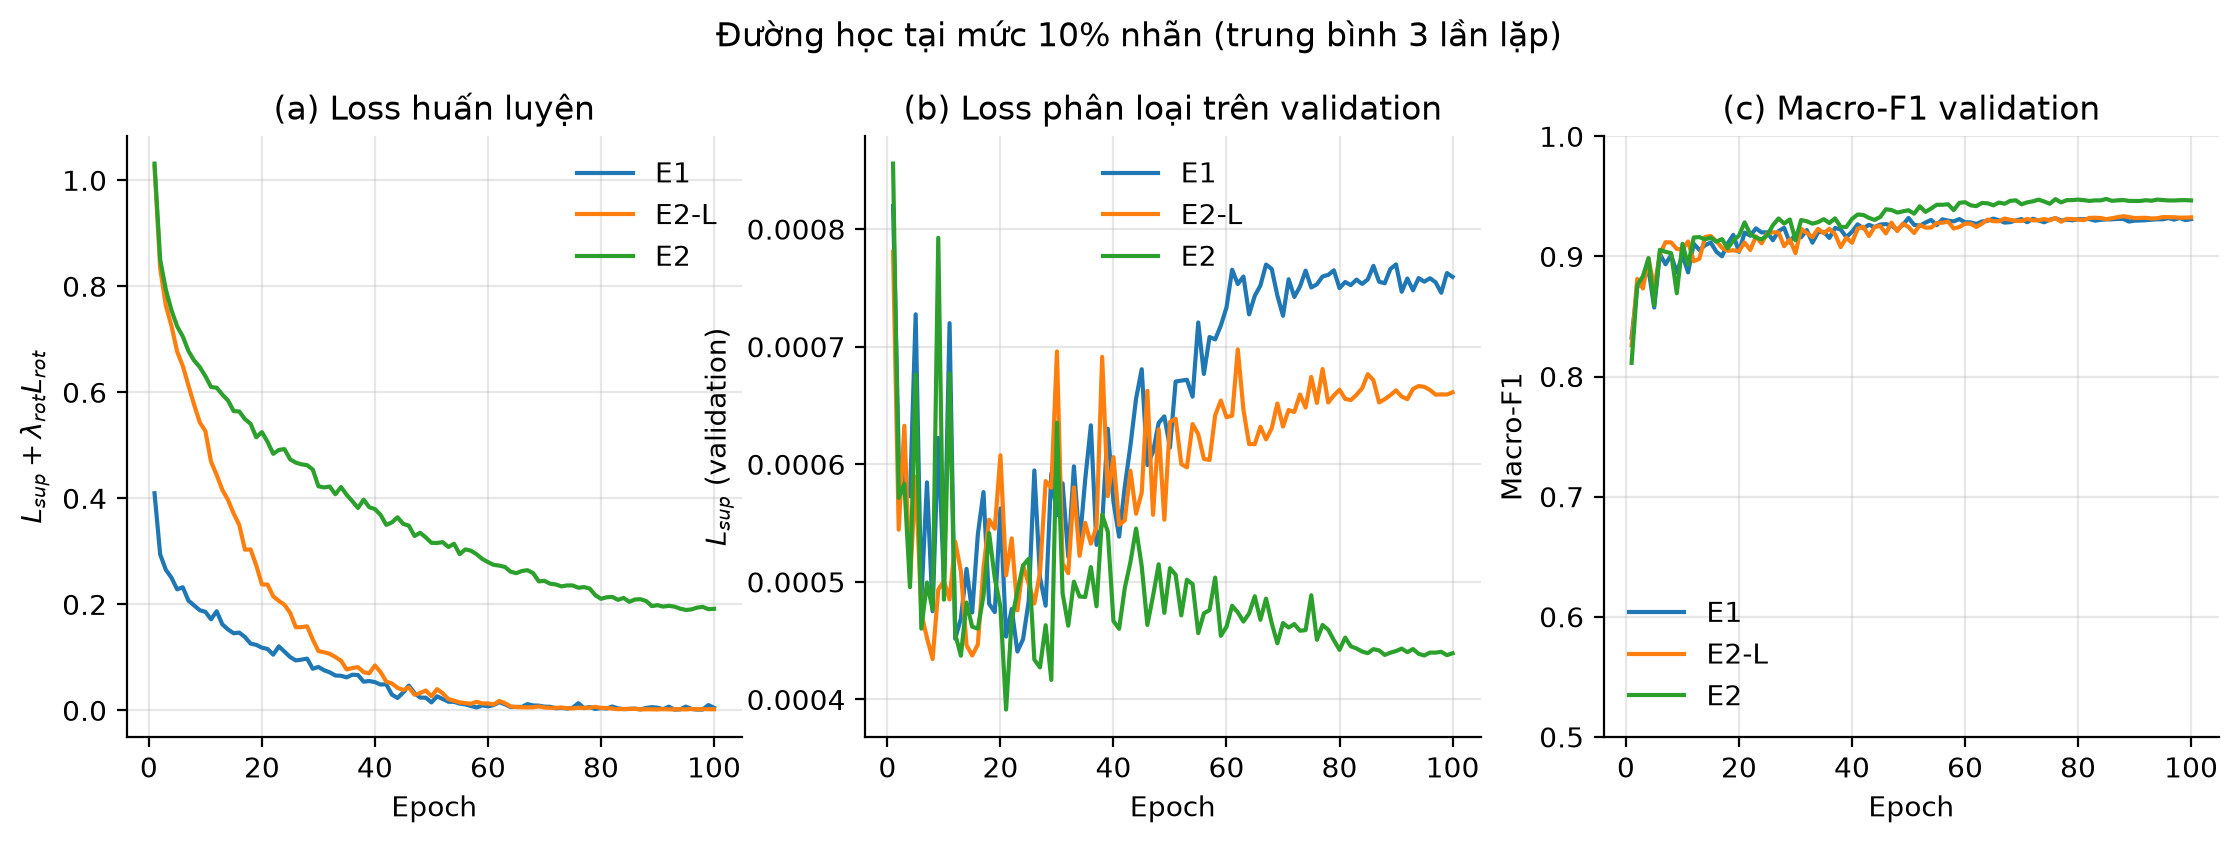
\includegraphics[width=\textwidth]{../results/figures/fig01_learning_curves_L10.png}
  \caption{Đường học tại mức $10\,\%$ nhãn, trung bình qua ba lần lặp. (a)~Loss huấn luyện
  gồm cả hai nhánh; (b)~loss phân loại trên validation; (c)~Macro-F1 validation. Ở cấu hình
  \cfg{E1} nhánh phụ không tồn tại nên $L_{\mathrm{rot}}$ không được định nghĩa.}
  \label{fig:learning-curves}
\end{figure}

\subsection{Chênh lệch ghép cặp}
\label{sec:results-delta}

Vì ba lần lặp tương ứng với ba tập con nhãn khác nhau, phép so sánh có ý nghĩa nhất là so sánh
\emph{ghép cặp}: tính $\Delta_s$ cho từng lần lặp rồi mới tổng hợp, thay vì so sánh hai trung
bình độc lập. \tabref{tab:main-results} đã ghi giá trị trung bình của $\Delta$; hình
\ref{fig:paired-delta} cho thấy phân bố của $\Delta_s$ theo từng lần lặp, nhờ đó có thể thấy
mức độ nhất quán của hiệu ứng.

\begin{figure}[htbp]
  \centering
  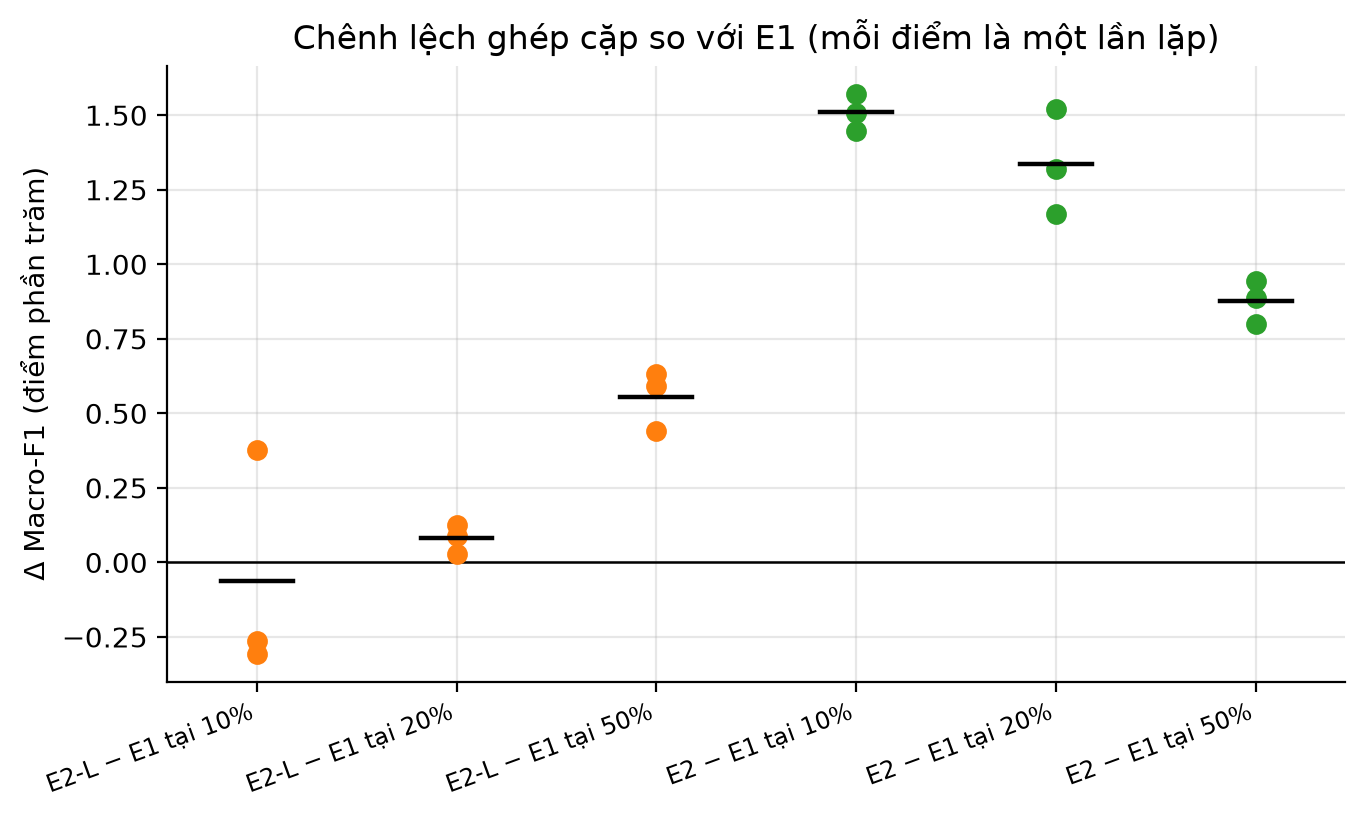
\includegraphics[width=0.95\textwidth]{../results/figures/fig03_paired_delta.png}
  \caption{Chênh lệch ghép cặp $\Delta_s$ so với \cfg{E1} ở cùng mức nhãn, tính bằng điểm phần
  trăm Macro-F1 trên $\Dtest$. Mỗi điểm là một lần lặp; vạch ngang là trung bình của ba lần
  lặp. Giá trị dương nghĩa là cấu hình đa nhiệm tốt hơn baseline.}
  \label{fig:paired-delta}
\end{figure}

\subsection{Hành vi hội tụ}
\label{sec:results-convergence}

Vì bảng kết quả chính không dùng Early Stopping, cần kiểm tra xem việc chạy đủ 100 epoch có dẫn
tới quá khớp lâu dài trên validation hay không. \tabref{tab:convergence} trình bày thời điểm đạt
checkpoint tốt nhất và mức suy giảm về cuối quá trình.

% Sinh tự động — scripts/make_report_data.py
\begin{table}[htbp]
  \centering
  \scriptsize
  \setlength{\tabcolsep}{4pt}
  \begin{tabular}{@{}l c c c r@{}}
    \toprule
    \makecell[l]{Cấu hình} & \makecell{Epoch\\tốt nhất} & \makecell{Macro-F1 val\\tại epoch tốt nhất} & \makecell{Macro-F1 val\\tại epoch cuối} & \makecell[r]{Khoảng\\cách} \\
    \midrule
    \cfg{E1} & 90,8 & 0,9521 & 0,9507 & +0,0014 \\
    \cfg{E2-L} & 85,3 & 0,9542 & 0,9524 & +0,0018 \\
    \cfg{E2} & 85,0 & 0,9644 & 0,9631 & +0,0014 \\
    \bottomrule
  \end{tabular}
  \caption{Hành vi hội tụ. \enquote{Khoảng cách} là Macro-F1 validation tại epoch tốt nhất trừ giá trị tại epoch cuối; giá trị dương nghĩa là mô hình bắt đầu suy giảm trên validation trước khi kết thúc 100 epoch. Vì không dùng Early Stopping, quá trình vẫn chạy tới epoch 100 như thiết kế.}
  \label{tab:convergence}
\end{table}

\subsection{Chỉ số từng lớp và phân tích lỗi}
\label{sec:results-perclass}

% Sinh tự động — scripts/make_report_data.py
\begin{table}[htbp]
  \centering
  \small
  \setlength{\tabcolsep}{6pt}
  \begin{tabular}{@{}l r r r r r@{}}
    \toprule
    & \multicolumn{2}{c}{Animal} & \multicolumn{2}{c}{Vehicle} & \\
    \cmidrule(lr){2-3}\cmidrule(lr){4-5}
    Cấu hình & Precision & Recall & Precision & Recall & F1 (Animal / Vehicle) \\
    \midrule
    \cfg{E1} & 0,9405 & 0,9517 & 0,9263 & 0,9096 & 0,9461 / 0,9178 \\
    \cfg{E2-L} & 0,9454 & 0,9447 & 0,9172 & 0,9181 & 0,9450 / 0,9176 \\
    \cfg{E2} & 0,9548 & 0,9608 & 0,9407 & 0,9318 & 0,9578 / 0,9362 \\
    \bottomrule
  \end{tabular}
  \caption{Precision, recall và F1 từng siêu lớp tại mức 10\,\% nhãn (trung bình ba lần lặp). Vì tỷ lệ Animal/Vehicle là 60/40, Accuracy đơn lẻ không phản ánh đầy đủ chất lượng của từng lớp.}
  \label{tab:per-class}
\end{table}

% Sinh tự động — scripts/make_report_data.py
\begin{table}[htbp]
  \centering
  \small
  \setlength{\tabcolsep}{6pt}
  \begin{tabular}{@{}l r r r r r@{}}
    \toprule
    & \multicolumn{2}{c}{Animal} & \multicolumn{2}{c}{Vehicle} & \\
    \cmidrule(lr){2-3}\cmidrule(lr){4-5}
    Cấu hình & Precision & Recall & Precision & Recall & F1 (Animal / Vehicle) \\
    \midrule
    \cfg{E1} & 0,9735 & 0,9769 & 0,9652 & 0,9602 & 0,9752 / 0,9627 \\
    \cfg{E2-L} & 0,9819 & 0,9772 & 0,9660 & 0,9730 & 0,9795 / 0,9695 \\
    \cfg{E2} & 0,9838 & 0,9805 & 0,9709 & 0,9758 & 0,9821 / 0,9733 \\
    \bottomrule
  \end{tabular}
  \caption{Precision, recall và F1 từng siêu lớp tại mức 50\,\% nhãn (trung bình ba lần lặp). Vì tỷ lệ Animal/Vehicle là 60/40, Accuracy đơn lẻ không phản ánh đầy đủ chất lượng của từng lớp.}
  \label{tab:per-class-50}
\end{table}

\begin{figure}[htbp]
  \centering
  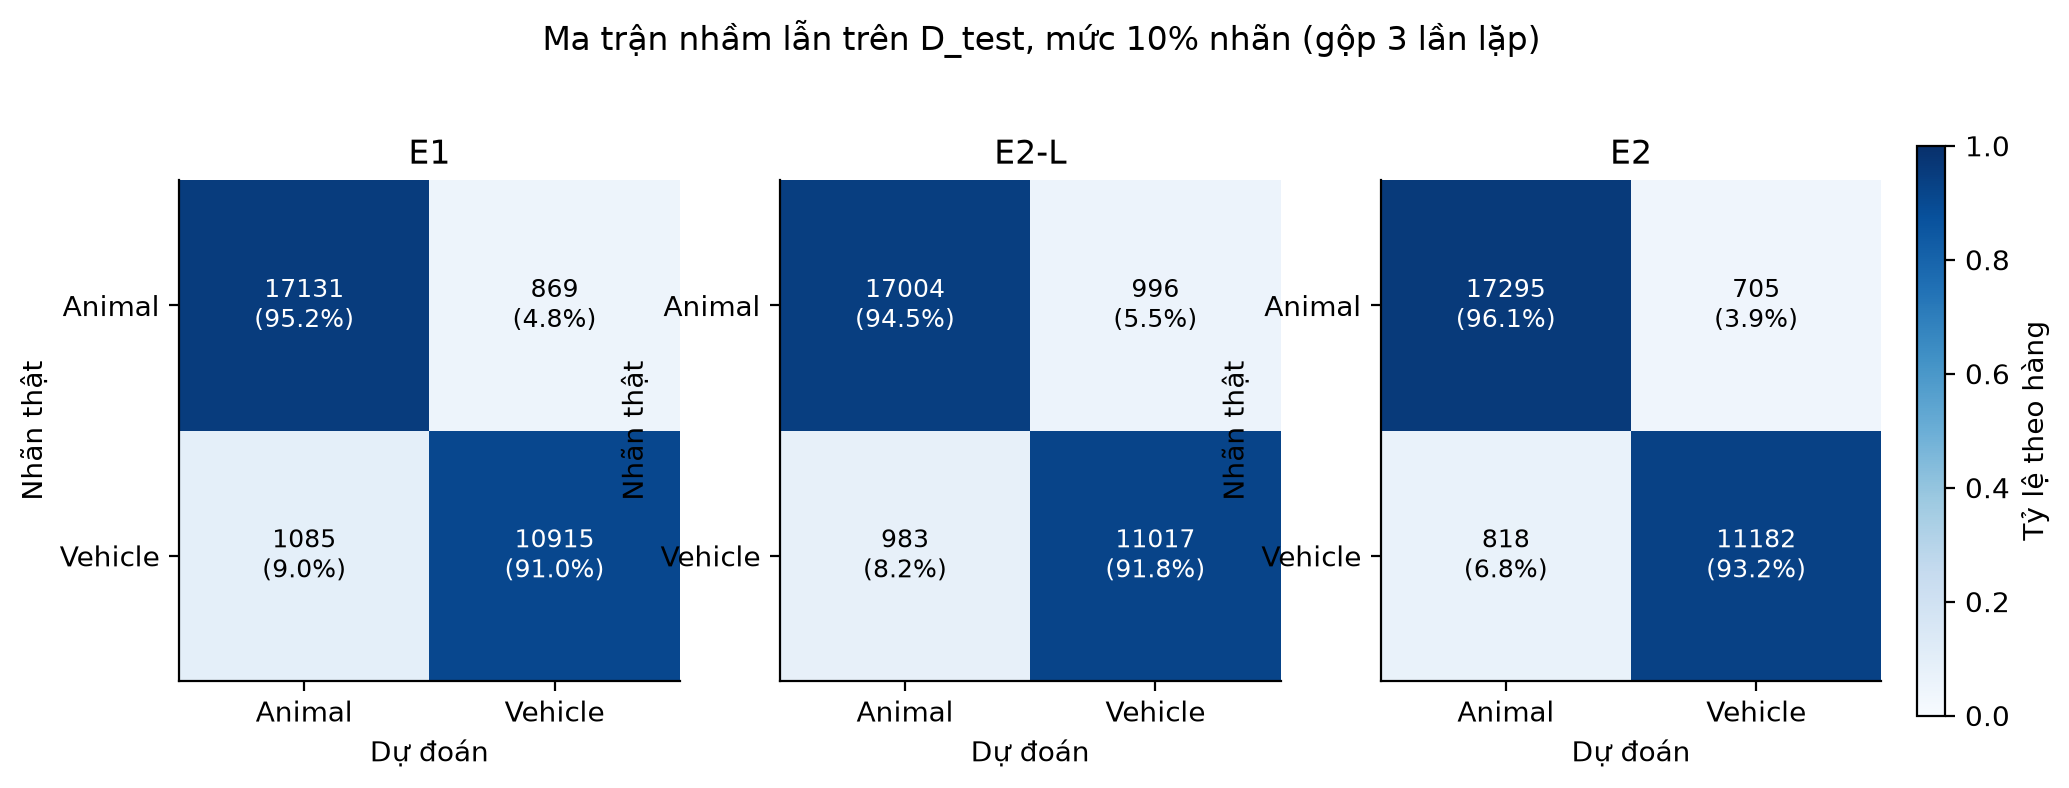
\includegraphics[width=\textwidth]{../results/figures/fig04_confusion_L10.png}
  \caption{Ma trận nhầm lẫn trên $\Dtest$ tại mức $10\,\%$ nhãn, gộp ba lần lặp (tổng 30.000
  dự đoán cho mỗi cấu hình). Ô ghi số lượng tuyệt đối và tỷ lệ theo hàng. Ma trận cho thấy
  phần lớn sai số tập trung ở lớp Vehicle bị dự đoán thành Animal.}
  \label{fig:confusion}
\end{figure}

\subsection{Chi phí huấn luyện và suy luận}
\label{sec:results-cost}

% Sinh tự động — scripts/make_report_data.py
\begin{table}[htbp]
  \centering
  \small
  \begin{tabular}{@{}l r r r@{}}
    \toprule
    Cấu hình & 10\,\% (giây/lượt) & 20\,\% (giây/lượt) & 50\,\% (giây/lượt) \\
    \midrule
    \cfg{E1} & 344,1 & 557,9 & 1.165,4 \\
    \cfg{E2-L} & 575,5 & 1.026,8 & 2.322,4 \\
    \cfg{E2} & 578,8 & 1.013,9 & 2.322,3 \\
    \bottomrule
  \end{tabular}
  \caption{Thời gian huấn luyện trung bình cho một lượt chạy 100 epoch. \cfg{E2-L} và \cfg{E2} xử lý thêm minibatch cho nhiệm vụ xoay ở mỗi bước cập nhật, nên chi phí học cao hơn \cfg{E1} một cách có hệ thống.}
  \label{tab:training-cost}
\end{table}

% Sinh tự động — scripts/make_report_data.py
\begin{table}[htbp]
  \centering
  \small
  \begin{tabular}{@{}l r@{}}
    \toprule
    Thành phần & Giá trị \\
    \midrule
    Tham số encoder $\enc$ & 11.168.832 \\
    Tham số Superclass Head & 1.026 \\
    Tham số Rotation Head & 2.052 \\
    Tổng tham số khi suy luận & \RParamInference \\
    Tổng tham số khi huấn luyện & \RParamTraining \\
    Dung lượng FP32 của mô hình suy luận & \RParamInferenceMiB{} MiB \\
    Dung lượng tệp trọng số suy luận đo được & \RParamInferenceFileMiB{} MiB \\
    \bottomrule
  \end{tabular}
  \caption{Chi phí tham số của mô hình tại cấu hình \secref{sec:arch}. Rotation Head chỉ tồn tại trong giai đoạn huấn luyện; khi suy luận chỉ cần encoder và Superclass Head. Dung lượng tệp được đo bằng cách lưu riêng trọng số suy luận, không gộp optimizer state.}
  \label{tab:inference-cost}
\end{table}

\paragraph{Vì sao \cfg{E2} đắt hơn \cfg{E2-L} — và vì sao khoảng cách đó thu hẹp theo mức nhãn.}
\tabref{tab:rotation-data-cost} đo riêng chi phí \emph{dựng view} của nhánh phụ. Ở mức
$10\,\%$ nhãn, nguồn $\Dtrain$ gấp $10$ lần nguồn $\DL$ về số view mỗi epoch; ở mức $50\,\%$
nhãn, tỷ lệ này chỉ còn $2$ lần. Đây là lý do định lượng cho việc \cfg{E2} đắt hơn \cfg{E2-L}
rõ rệt khi ít nhãn.

% Sinh tự động — scripts/make_report_data.py
\begin{table}[htbp]
  \centering
  \small
  \setlength{\tabcolsep}{6pt}
  \begin{tabular}{@{}r r r r r@{}}
    \toprule
    Mức nhãn & $|\DL|$ (view) & $|\Dtrain|$ (view) & Giây/epoch khi nguồn $= \DL$ & Giây/epoch khi nguồn $= \Dtrain$ \\
    \midrule
    10\,\% & 4.500 & 45.000 & 1,2 & 13,2 \\
    20\,\% & 9.000 & 45.000 & 2,7 & 13,7 \\
    50\,\% & 22.500 & 45.000 & 6,8 & 13,6 \\
    \bottomrule
  \end{tabular}
  \caption{Chi phí \emph{dựng view} cho nhánh xoay, đo riêng trên CPU, không gồm forward/backward. Bảng đo theo GIẢ ĐỊNH nhánh phụ duyệt hết tập nguồn mỗi epoch; trong mã nguồn thì $B_R$ được cắt về đúng $b_L$, nên số view \emph{thực dùng} mỗi epoch bằng $|\DL|$ ở cả \cfg{E2-L} và \cfg{E2}. Vì vậy chi phí dựng view thực tế của hai cấu hình gần như bằng nhau, và tỷ lệ nêu trên là chi phí của kịch bản giả định.}
  \label{tab:rotation-data-cost}
\end{table}

% Sinh tự động — scripts/make_report_data.py
\begin{table}[htbp]
  \centering
  \small
  \begin{tabular}{@{}l r r r@{}}
    \toprule
    Điều kiện đo & Mean (ms/ảnh) & Median (ms/ảnh) & p95 (ms/ảnh) \\
    \midrule
    CPU (4 luồng), FP32 & \RLatMeanCpu & \RLatMedianCpu & \RLatPNinetyFiveCpu \\
    GPU (RTX 5070 Laptop), FP32 & \RLatMeanGpu & \RLatMedianGpu & \RLatPNinetyFiveGpu \\
    \bottomrule
  \end{tabular}
  \caption{Độ trễ suy luận với batch $=1$, tensor $1 \times 3 \times 32 \times 32$, FP32, \code{model.eval()} và \code{torch.inference\_mode()}. Mỗi điều kiện khởi động 50 lượt rồi đo 1.000 lượt, lặp ba phiên. Cách tổng hợp ba phiên KHÔNG giống nhau: \emph{mean} và \emph{p95} là trung bình cộng của ba phiên, còn \emph{median} là trung vị của ba trung vị phiên (xem \code{src/m8/benchmark.py}). Phép đo chỉ tính thời gian tính toán của mô hình, không gồm đọc ảnh và tiền xử lý.}
  \label{tab:latency}
\end{table}

\paragraph{Đọc các số liệu chi phí.}
Độ trễ trung bình \RLatMeanCpu{}~ms/ảnh trên CPU (ghim \RLatThreads{} luồng) và
\RLatMeanGpu{}~ms/ảnh trên \REnvGpu{} ở chế độ đo đã đồng bộ CUDA. Con số p95 trên GPU
(\RLatPNinetyFiveGpu{}~ms) cao hơn trung vị (\RLatMedianGpu{}~ms) cho thấy phân bố thời gian không đối
xứng: một số lượt đo bị chi phối bởi chi phí phát lệnh và đồng bộ chứ không phải bởi phép tính
thực sự của mạng trên tensor nhỏ $1 \times 3 \times 32 \times 32$. Thời gian đọc ảnh và tiền xử
lý trên CPU được đo riêng và có giá trị \RPreprocessMs{}~ms/ảnh, tức cùng bậc độ lớn với thời
gian suy luận GPU; đây là yếu tố thường bị bỏ qua khi chỉ báo cáo \enquote{độ trễ mô hình}.

\paragraph{So sánh chi phí học giữa ba cấu hình.}
\tabref{tab:training-cost} cho thấy \cfg{E1} rẻ nhất, \cfg{E2-L} và \cfg{E2} đắt hơn do phải
xử lý thêm một minibatch ở mỗi bước cập nhật. Cần lưu ý rằng mức tăng này không tỷ lệ với số
epoch (cả ba cấu hình đều 100 epoch) mà tỷ lệ với số lượt ảnh được xử lý.

% =====================================================================
\section{Kết quả phần mở rộng: Contrastive Learning và SupCon}
\label{sec:results-ext}
% =====================================================================

Phần này trình bày khối mở rộng tùy chọn \cfg{E3}--\cfg{E6} đã mô tả tại
\secref{sec:contrastive}, chạy \emph{sau} khi khối đối chứng chính đã hoàn tất. Đây là phần
nằm ngoài yêu cầu bắt buộc của đề cương, nên mọi kết luận ở đây được trình bày như
\textbf{bằng chứng thăm dò} chứ không phải kết luận của đề tài.

\subsection{Nguyên tắc khóa siêu tham số}
\label{sec:results-ext-lambda}

Điều khoản 4.2 của đề cương yêu cầu khóa siêu tham số mở rộng bằng validation trước khi đánh
giá test, và cấm lựa chọn cấu hình dựa trên kết quả test. Vì vậy quy trình được chia thành hai
bước tách bạch về mặt thông tin:

\begin{enumerate}[label=\textbf{B\arabic*.},leftmargin=1.4cm,itemsep=3pt]
  \item \textbf{Khảo sát chỉ trên validation.} Chạy \cfg{E4} và \cfg{E6} tại mức
        $10\,\%$ nhãn, seed 42, với $\lamc \in \{0{,}05;\ 0{,}1;\ 0{,}25;\ 0{,}5;\ 1{,}0\}$.
        Script khảo sát (\code{scripts/sweep\_lambda\_c.py}) \textbf{không gọi} bước đánh giá
        test, nên kết quả test không thể ảnh hưởng tới quyết định.
  \item \textbf{Khóa $\lamc$} theo một quy tắc khai báo trước: chọn \emph{một} giá trị dùng
        chung cho mọi cấu hình mở rộng (đúng như bảng 5 của đề cương) sao cho \emph{trung bình}
        Macro-F1 validation qua hai cấu hình khảo sát là lớn nhất. Quy tắc này được chọn vì mỗi
        cấu hình có cực trị riêng (xem \tabref{tab:lambda-sweep}); khóa theo một cấu hình duy
        nhất có thể rất kém cho cấu hình còn lại.
\end{enumerate}

% Sinh tự động — scripts/make_report_data.py
\begin{table}[htbp]
  \centering
  \small
  \begin{tabular}{@{}l c c c c c@{}}
    \toprule
    Cấu hình & $\lambda_c = 0,05$ & $\lambda_c = 0,10$ & $\lambda_c = 0,25$ & $\lambda_c = 0,50$ & $\lambda_c = 1,00$ \\
    \midrule
    \cfg{E4} & 0,9266 & 0,9354 & 0,9352 & 0,9425 & 0,9454 \\
    \cfg{E6} & 0,9391 & 0,9418 & 0,9496 & 0,9457 & 0,9468 \\
    \midrule
    \textit{được khóa} &  &  &  &  & $\bullet$ \\
    \bottomrule
  \end{tabular}
  \caption{Khảo sát $\lambda_c$ bằng \textbf{Macro-F1 validation} với 40 epoch, mức 10\,\% nhãn, seed 42. Tập test \textbf{không} được đánh giá trong bước này. Quy tắc khóa được khai báo trước: chọn \emph{một} $\lambda_c$ dùng chung cho mọi cấu hình mở rộng sao cho trung bình Macro-F1 validation qua hai cấu hình khảo sát là lớn nhất; giá trị được chọn là 1,00 (trung bình 0,9461).}
  \label{tab:lambda-sweep}
\end{table}

\figref{fig:lambda-sweep} cho thấy toàn bộ đường khảo sát. Đáng lưu ý, cả hai hàm mất mát đều
\emph{nhạy} với $\lamc$: chênh lệch giữa giá trị tốt nhất và xấu nhất trong lưới khảo sát là
khoảng $2$ điểm phần trăm Macro-F1 validation. Điều này khẳng định việc chạy khảo sát là cần
thiết, thay vì chọn $\lamc$ theo trực giác.

\begin{figure}[htbp]
  \centering
  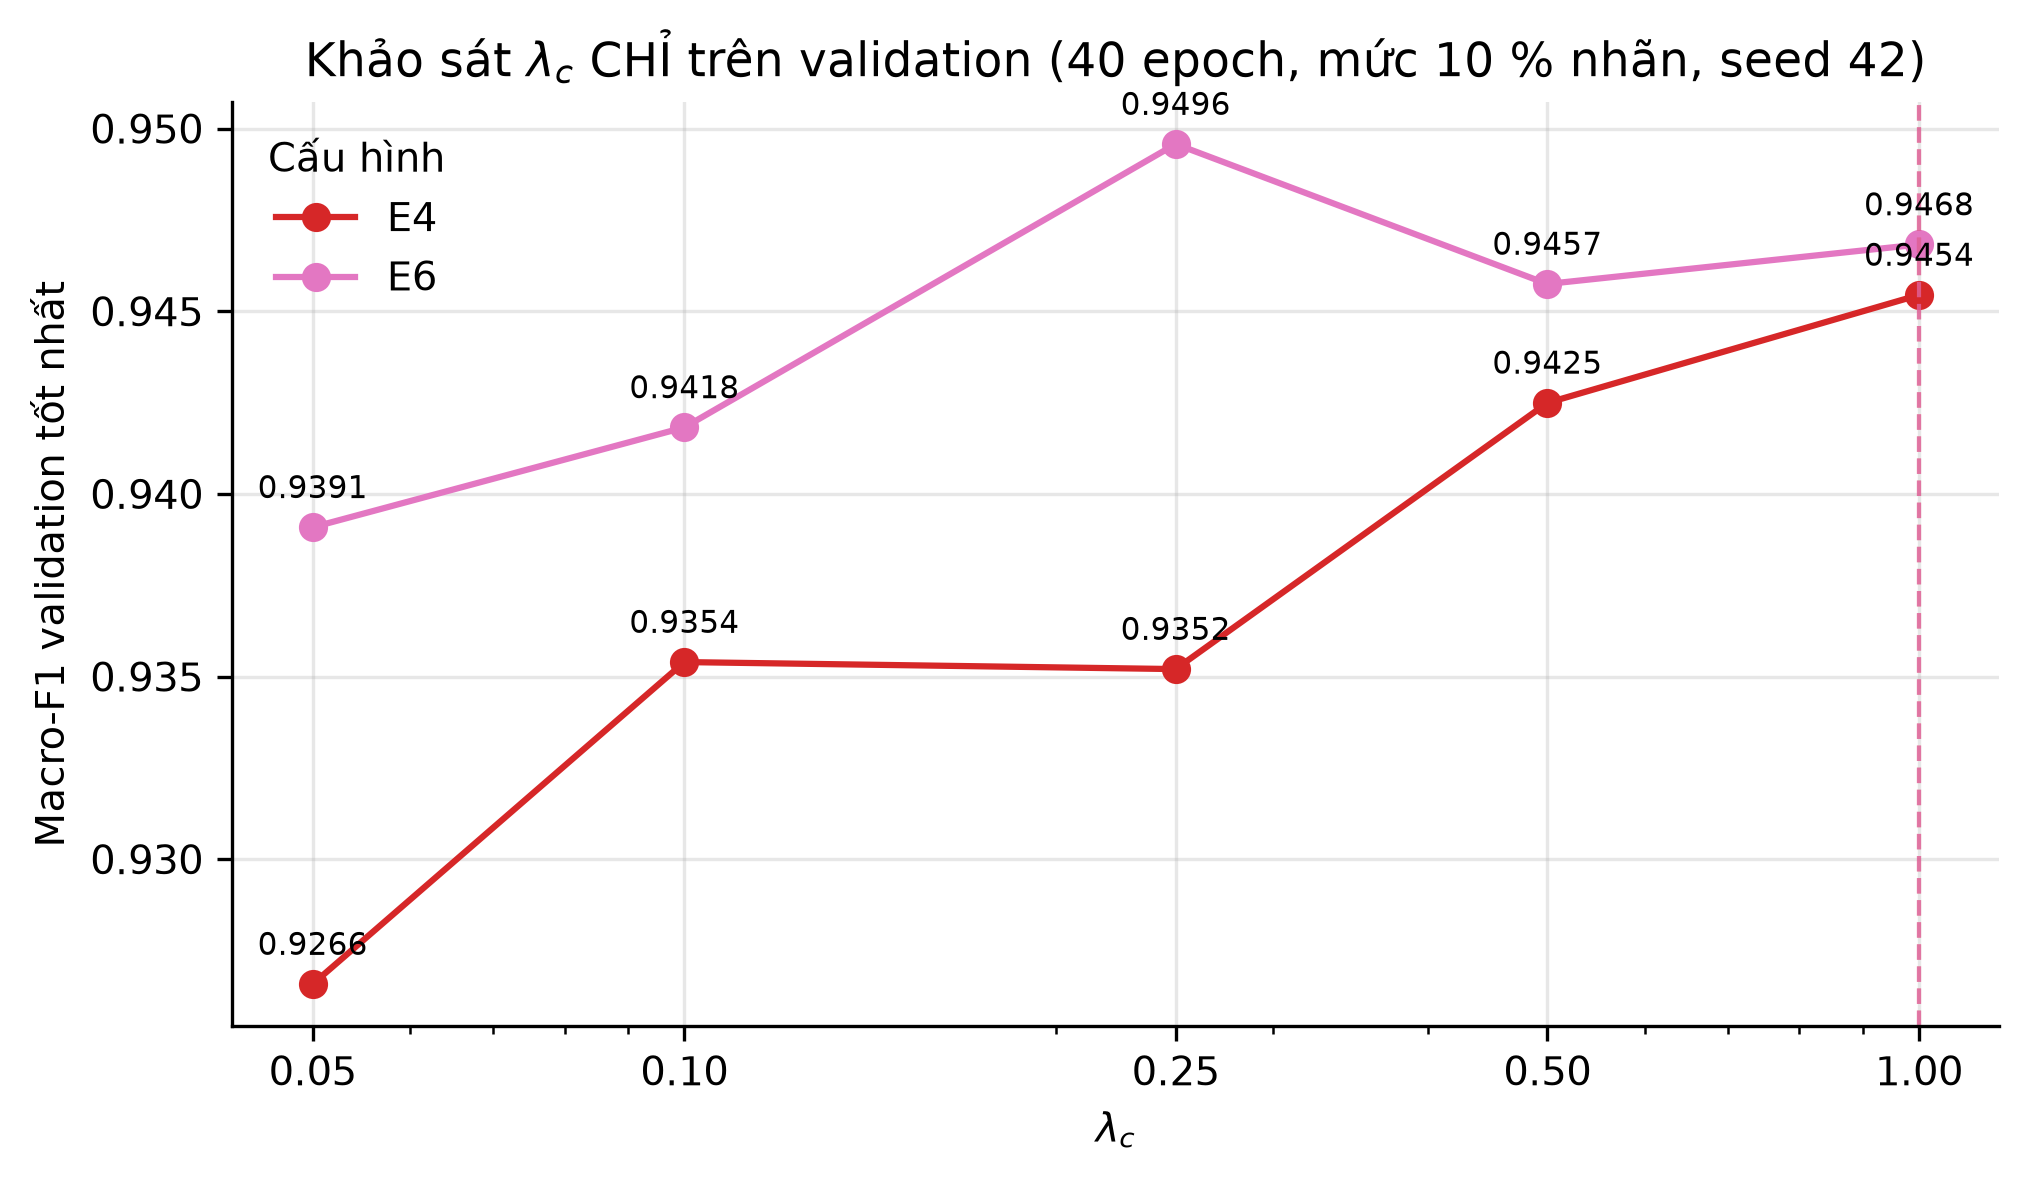
\includegraphics[width=0.92\textwidth]{../results/figures/fig08_lambda_sweep.png}
  \caption{Khảo sát $\lamc$ \textbf{chỉ trên Macro-F1 validation} (40 epoch, mức
  $10\,\%$ nhãn, seed 42). Đường đứt dọc là giá trị được khóa. Tập test không được đánh giá
  trong bước này.}
  \label{fig:lambda-sweep}
\end{figure}

\subsection{Kết quả và đối chứng ghép cặp}
\label{sec:results-ext-main}

Sau khi khóa $\lamc$, bốn cấu hình được chạy tại mức nhãn \textbf{$10\,\%$} với ba lần lặp
42, 43, 44 — tổng cộng $4 \times 3 = 12$ lượt huấn luyện 100 epoch. Mức $10\,\%$ được chọn vì
đây là mức ưu tiên của đề cương (mục 4.2) và là mức mà phần bắt buộc cho thấy độ biến động lớn
nhất giữa các cấu hình. Mỗi lượt vẫn giữ đúng giao thức của khối chính: 100 epoch, AdamW, chọn
checkpoint bằng Macro-F1 validation, không Early Stopping, không dùng test-time augmentation.

\begin{keybox}
\textbf{Giới hạn phạm vi.} Khối mở rộng chỉ được chạy ở mức $10\,\%$ nhãn; hai mức $20\,\%$ và
$50\,\%$ \textbf{không} được khảo sát cho \cfg{E3}--\cfg{E6}. Vì vậy mọi kết luận ở
\secref{sec:results-ext} \emph{chỉ} áp dụng cho mức $10\,\%$ nhãn, kiến trúc và giao thức đã mô
tả. So sánh với \cfg{E1} vẫn hợp lệ vì \cfg{E1} có kết quả đầy đủ ở cả ba mức nhãn.
\end{keybox}

% Sinh tự động — scripts/make_report_data.py
\begin{table}[htbp]
  \centering
  \scriptsize
  \setlength{\tabcolsep}{4.5pt}
  \begin{tabular}{@{}l r r r r r r@{}}
    \toprule
    & \multicolumn{2}{c}{10\,\% nhãn} & \multicolumn{2}{c}{20\,\% nhãn} & \multicolumn{2}{c}{50\,\% nhãn} \\
    \cmidrule(lr){2-3}\cmidrule(lr){4-5}\cmidrule(lr){6-7}
    Cấu hình & Macro-F1 & $\Delta$ & Macro-F1 & $\Delta$ & Macro-F1 & $\Delta$ \\
    \midrule
    \cfg{E1} & 0,9319 & --- & 0,9497 & --- & 0,9690 & --- \\
    \addlinespace[2pt]
    \cfg{E2-L} & 0,9313 & $-$0,06 & 0,9505 & +0,08 & 0,9745 & +0,55 \\
    \addlinespace[2pt]
    \cfg{E2} & 0,9470 & +1,51 & 0,9631 & +1,34 & 0,9777 & +0,88 \\
    \cfg{E3} & 0,9438 & +1,19 & --- & --- & --- & --- \\
    \cfg{E4} & 0,9527 & +2,07 & --- & --- & --- & --- \\
    \cfg{E5} & 0,9496 & +1,77 & --- & --- & --- & --- \\
    \cfg{E6} & 0,9579 & +2,60 & --- & --- & --- & --- \\
    \bottomrule
  \end{tabular}
  \caption{Kết quả trên $\Dtest$, trung bình qua ba lần lặp. $\Delta$ là chênh lệch Macro-F1 ghép cặp so với \cfg{E1} ở cùng mức nhãn, đơn vị điểm phần trăm. Hai nhóm được ngăn bằng khoảng trắng: \cfg{E1}/\cfg{E2-L}/\cfg{E2} là khối chính; \cfg{E3}--\cfg{E6} là khối mở rộng contrastive.}
  \label{tab:extension-results}
\end{table}

\begin{figure}[htbp]
  \centering
  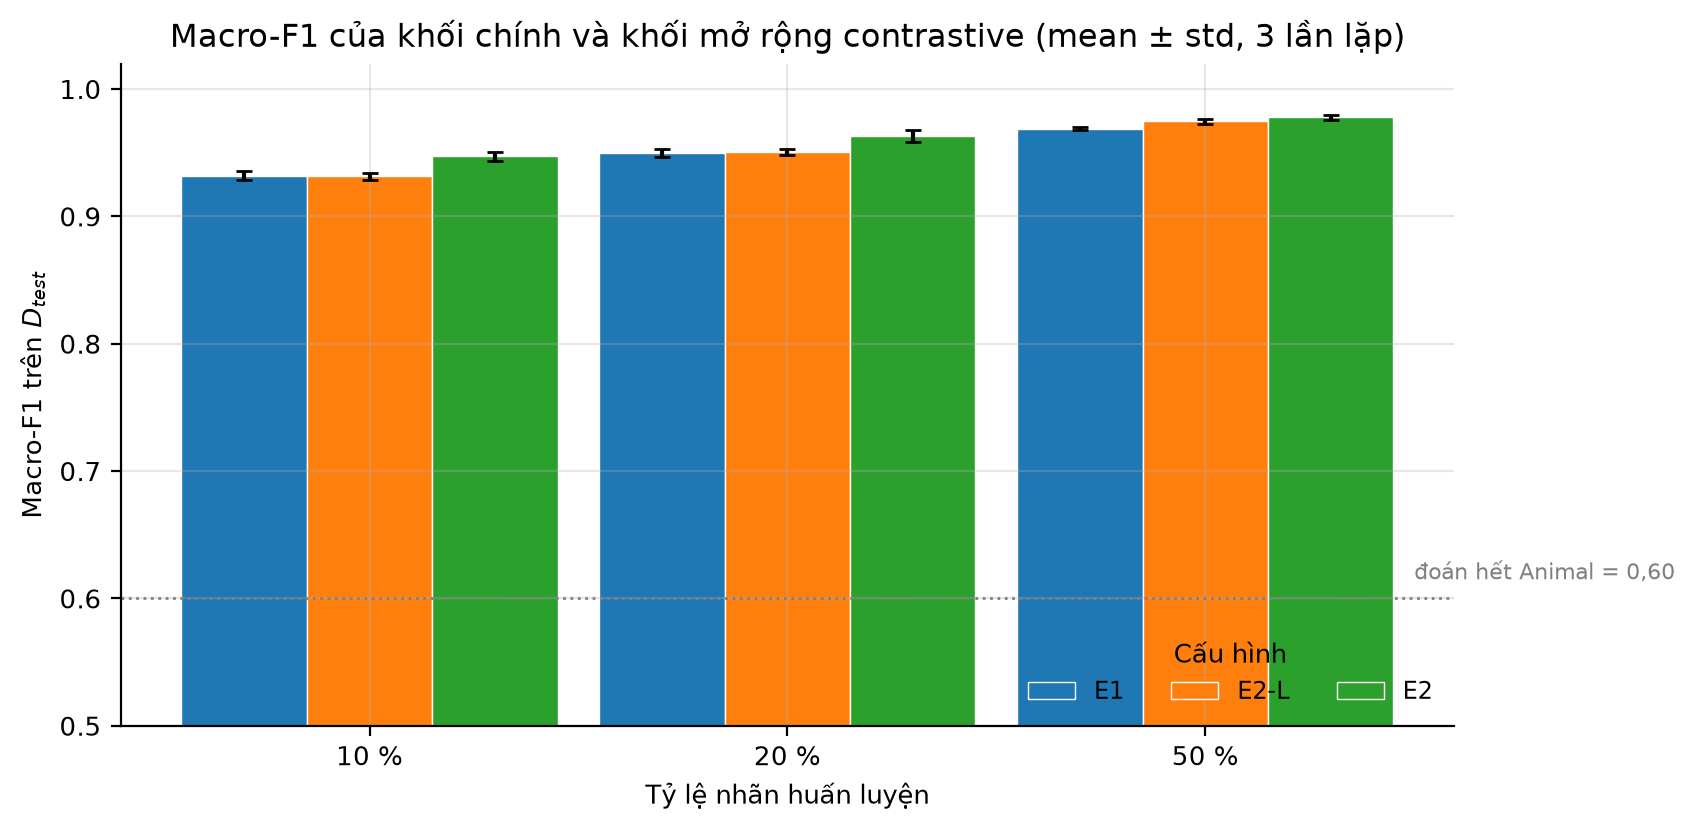
\includegraphics[width=\textwidth]{../results/figures/fig06_extension_macro_f1.png}
  \caption{Macro-F1 trên $\Dtest$ của các cấu hình \emph{đã có kết quả}, trung bình qua các lần
  lặp đã xong, so với mức $0{,}60$ của bộ phân loại luôn đoán Animal. Khối chính (\cfg{E1},
  \cfg{E2-L}, \cfg{E2}) có kết quả ở cả ba mức nhãn; khối mở rộng contrastive chỉ được khảo sát
  ở mức $10\,\%$ nhãn (xem \tabref{tab:extension-results}). Hình được sinh lại tự động bởi
  \code{scripts/make\_extension\_figures.py}, nên số cột phản ánh đúng số cấu hình đã chạy
  xong tại thời điểm sinh báo cáo.}
  \label{fig:extension-f1}
\end{figure}

\begin{figure}[htbp]
  \centering
  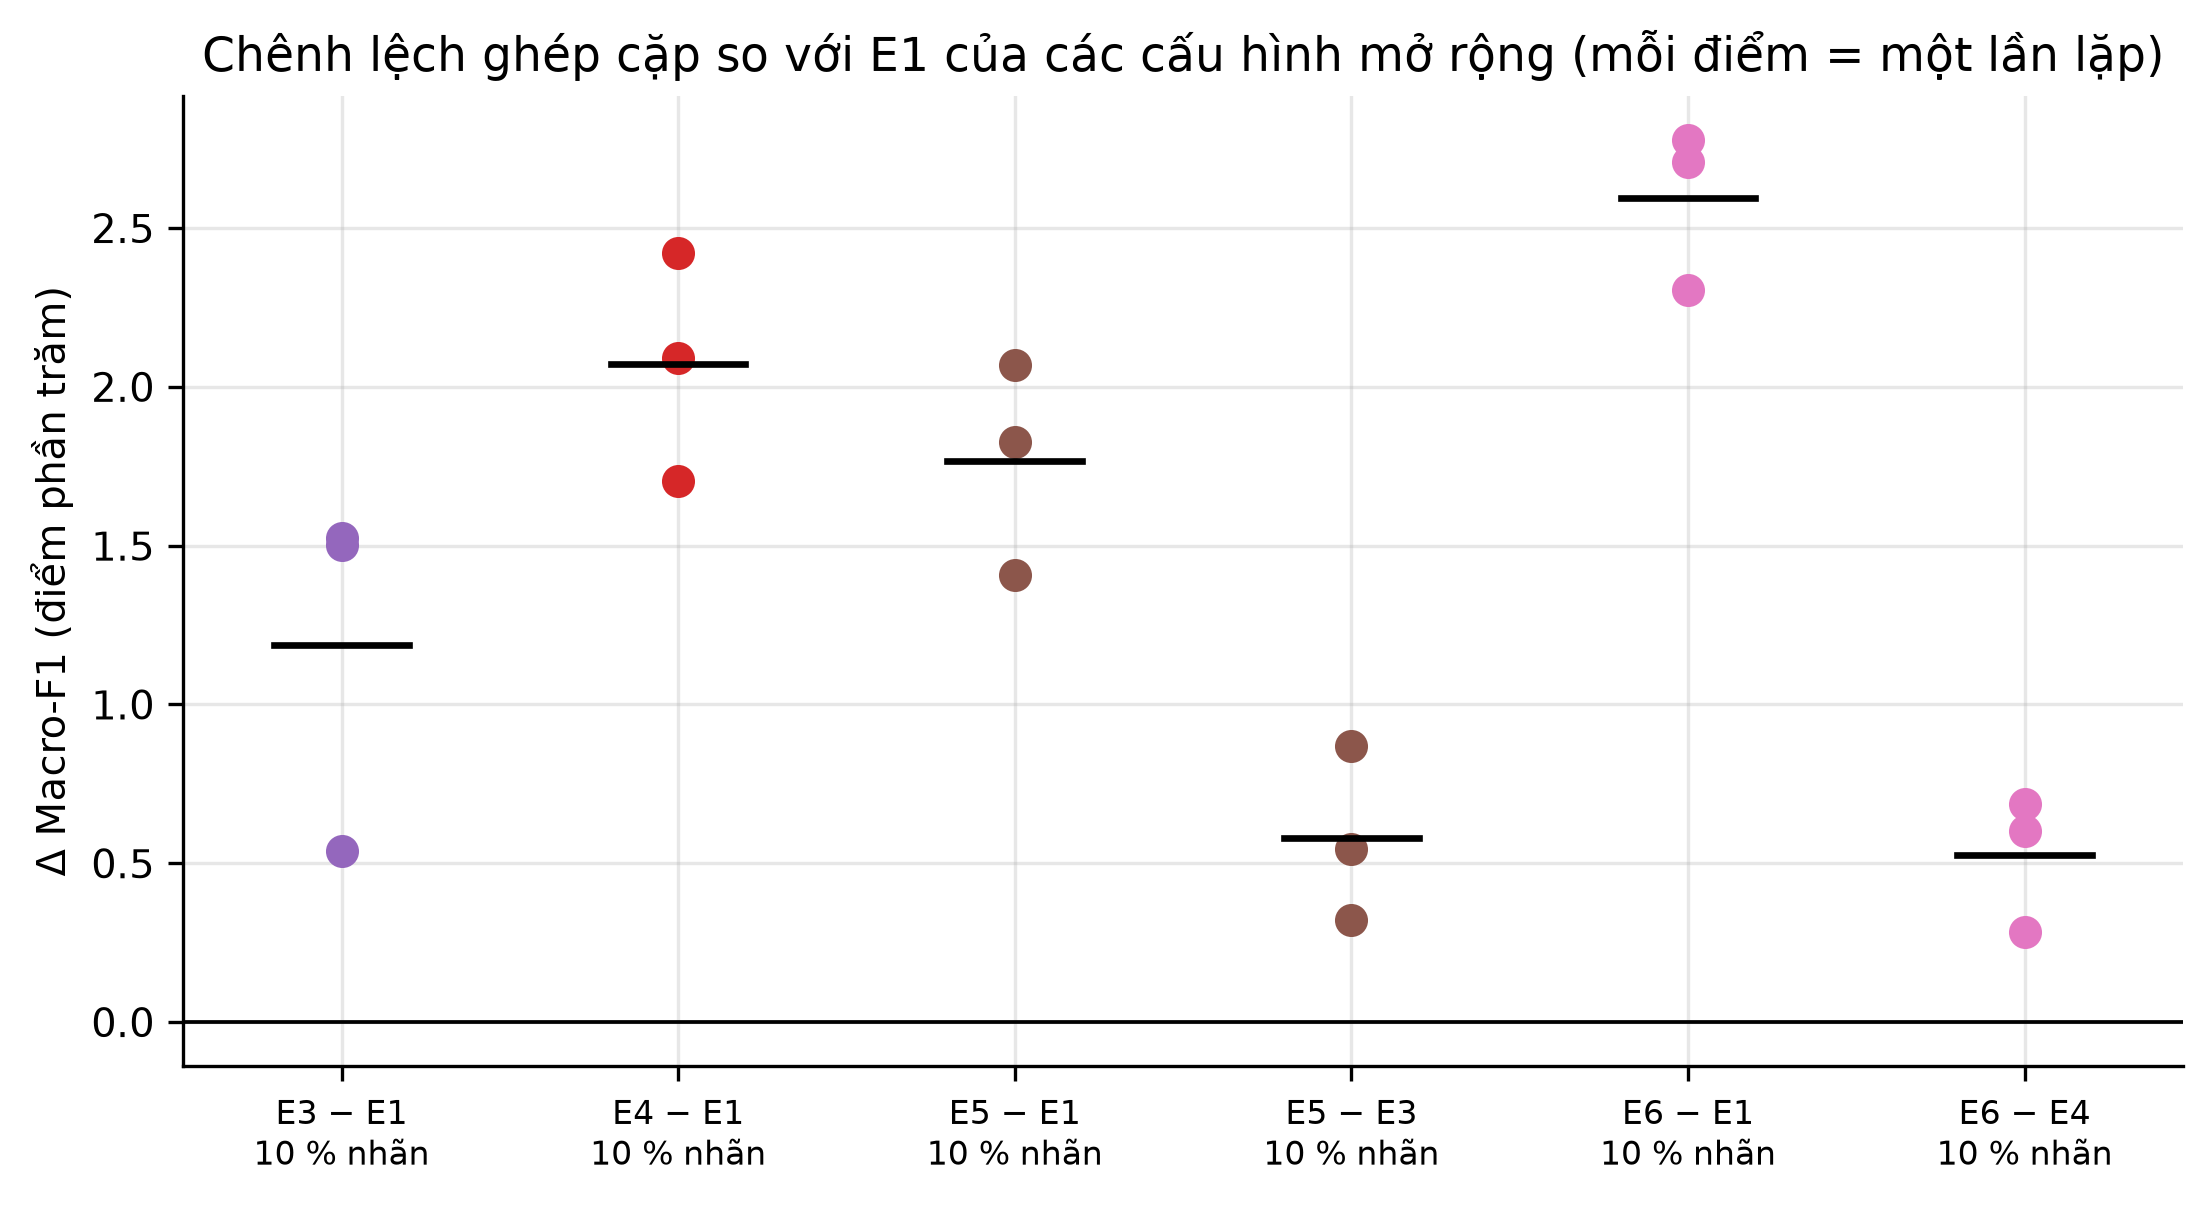
\includegraphics[width=\textwidth]{../results/figures/fig07_extension_delta.png}
  \caption{Chênh lệch ghép cặp $\Delta_s$ so với \cfg{E1} của từng cấu hình mở rộng, mỗi điểm
  là một lần lặp. Đường ngang là trung bình các lần lặp đã xong. Giá trị dương nghĩa là cấu hình
  đó tốt hơn baseline ở cùng ngân sách nhãn. Nếu chưa có lượt mở rộng nào thì hình chỉ hiển thị
  thông báo chưa có dữ liệu — đây là hình sinh tự động, không phải hình minh hoạ.}
  \label{fig:extension-delta}
\end{figure}

\subsection{Phân tích}
\label{sec:results-ext-analysis}

\RExtensionAnalysis

\subsection{Chi phí của phần mở rộng}
\label{sec:results-ext-cost}

% Sinh tự động — scripts/make_report_data.py
\begin{table}[htbp]
  \centering
  \scriptsize
  \setlength{\tabcolsep}{4pt}
  \begin{tabular}{@{}l r r r r r@{}}
    \toprule
    Cấu hình & \makecell[r]{Tham số\\suy luận} & \makecell[r]{Rotation\\Head} & \makecell[r]{Projection\\Head} & \makecell[r]{Giây/epoch\\(mức 10\,\%)} & \makecell[r]{Lượt ảnh phụ\\mỗi epoch\\(mức 10\,\%)} \\
    \midrule
    \cfg{E1} & 11.169.858 & 0 & 0 & 3,4 & 0 \\
    \cfg{E2-L} & 11.169.858 & 2.052 & 0 & 5,8 & 4.608 \\
    \cfg{E2} & 11.169.858 & 2.052 & 0 & 5,8 & 4.608 \\
    \cfg{E3} & 11.169.858 & 0 & 328.832 & 15,0 & 9.000 \\
    \cfg{E4} & 11.169.858 & 0 & 328.832 & 15,1 & 9.000 \\
    \cfg{E5} & 11.169.858 & 2.052 & 328.832 & 17,9 & 13.500 \\
    \cfg{E6} & 11.169.858 & 2.052 & 328.832 & 18,2 & 13.500 \\
    \bottomrule
  \end{tabular}
  \caption{Chi phí của khối mở rộng. Số tham số suy luận \textbf{không} thay đổi so với khối chính vì cả Rotation Head lẫn Projection Head đều bị bỏ khi suy luận. \enquote{Lượt ảnh phụ} là tổng số lượt ảnh mà các nhánh phụ xử lý trong một epoch; đây là lý do định lượng khiến các cấu hình mở rộng chậm hơn \cfg{E1}.}
  \label{tab:extension-cost}
\end{table}

\paragraph{Projection Head không làm mô hình suy luận lớn hơn.}
Bảng \ref{tab:extension-cost} cho thấy số tham số suy luận của mọi cấu hình \cfg{E3}--\cfg{E6}
vẫn đúng bằng \RParamInference{} như khối chính. Cả Rotation Head lẫn Projection Head đều
\textbf{bị bỏ hoàn toàn} khi suy luận, nên chi phí thêm chỉ là chi phí học một lần. Đây là
điểm khác biệt căn bản so với các kỹ thuật tăng kích thước mô hình để tăng độ chính xác.

\paragraph{Nhánh phụ đắt hơn trong giai đoạn học.}
Các nhánh phụ khiến mỗi bước cập nhật phải xử lý thêm ảnh: nhánh xoay xử lý một minibatch,
nhánh contrastive xử lý \emph{hai} view cho mỗi ảnh trong minibatch của nó. Vì mỗi epoch vẫn
chỉ duyệt $\DL$ một lần, thời gian mỗi epoch tăng gần như tuyến tính theo số lượt ảnh phụ.

\subsection{Kết luận của phần mở rộng}
\label{sec:results-ext-conclusion}

\RExtensionConclusion

% =====================================================================
\section{Thảo luận}
\label{sec:discussion}
% =====================================================================

\subsection{Trả lời ba câu hỏi đánh giá}
\label{sec:disc-answers}

\paragraph{C1 --- Hiệu quả phân loại.}
\RFindingCone

\paragraph{C2 --- Vai trò của dữ liệu cho nhiệm vụ phụ.}
\RFindingCtwo

\paragraph{C3 --- Chi phí thực hiện.}
\RFindingCthree

\subsection{Đọc kết quả theo hướng xu hướng ngân sách nhãn}
\label{sec:disc-trend}

Giả thuyết ban đầu cho rằng nhiệm vụ phụ có lợi nhất khi ít nhãn, vì lúc đó tín hiệu tự giám
sát bổ sung được thông tin mà nhãn có giám sát không cung cấp đủ. Hình~\ref{fig:macro-f1} cho
phép kiểm tra giả thuyết này bằng cách so sánh độ lớn của $\Delta$ ở ba mức $10\,\%$, $20\,\%$
và $50\,\%$. Điều cần chú ý là \emph{độ lớn của $\Delta$}, không chỉ dấu của nó: một cải thiện
$+0{,}3$ điểm phần trăm nằm trong cùng bậc độ lớn với độ lệch chuẩn quan sát được và do đó
không thể phân biệt với nhiễu.

\subsection{Các yếu tố gây nhiễu và mối đe dọa đến tính hợp lệ}
\label{sec:disc-threats}

\paragraph{Nhiễu do thống kê BatchNorm.}
\label{sec:exempt-bn}
Như đã nêu ở \secref{sec:arch}, encoder dùng chung các lớp BatchNorm cho cả hai nhánh. Khi so
sánh \cfg{E2-L} với \cfg{E1}, hai cấu hình khác nhau ở cả hàm mục tiêu \emph{lẫn} thành phần
của batch đi qua BatchNorm. Vì vậy $\Delta_s$ của phép so sánh này đo \emph{tổng hợp} tác dụng
của nhiệm vụ phụ và thay đổi chuẩn hóa, không tách riêng được hai thành phần. Đây là hệ quả của
một quyết định thiết kế kiến trúc (dùng chung BatchNorm là cần thiết để giảm số tham số và giữ
so sánh tham số ở mức ngang bằng), không phải lỗi cài đặt.

\paragraph{Nhiễu do chọn checkpoint bằng validation.}
Mọi cấu hình đều được chọn checkpoint bằng Macro-F1 validation cao nhất. Vì chỉ có 5.000 ảnh
validation, tiêu chí này có phương sai riêng: chênh lệch nhỏ về Macro-F1 test có thể chỉ phản
ánh việc \enquote{may mắn} khi chọn epoch. Việc dùng cùng tiêu chí cho mọi cấu hình làm giảm
nhưng không loại bỏ được vấn đề này.

\paragraph{Chỉ ba lần lặp.}
Ba lần lặp cho phép ước lượng một độ lệch chuẩn mẫu nhưng khoảng tin cậy vẫn rất rộng. Với
$n=3$, một chênh lệch trung bình bằng $0$ hoàn toàn tương thích với các lần lặp có $\Delta_s$
trái dấu. Do đó báo cáo này chỉ trình bày \emph{hướng} của hiệu ứng.

\paragraph{Phép chia dữ liệu cố định.}
Cả ba lần lặp dùng chung một tập validation và một tập test. Phương sai do chính phép chia gây
ra \textbf{không} được ước lượng. Muốn ước lượng thành phần này cần lặp lại cả phép chia, tức
tăng chi phí lên đáng kể.

\paragraph{Không dùng Early Stopping.}
Quyết định bỏ Early Stopping để bảo đảm số bước cập nhật có giám sát giống nhau. Đánh đổi là
một số lượt chạy có thể đã quá khớp (xem loss huấn luyện rất nhỏ ở cuối giai đoạn, ví dụ
$L_{\mathrm{sup}} < 0{,}01$ ở epoch 100 tại mức $10\,\%$ nhãn), và checkpoint được chọn gần
cuối quá trình. Đây là hành vi nhất quán giữa các cấu hình, nhưng số liệu cuối cùng không phản
ánh chất lượng tốt nhất mà cấu hình đó có thể đạt được dưới một chiến lược dừng khác.

\paragraph{Kích thước batch và chất lượng BatchNorm.}
Với $|\DL| = 4.500$ ở mức $10\,\%$, một epoch chỉ có 36 bước cập nhật. Số bước nhỏ làm cho
thống kê BatchNorm kém ổn định hơn so với trường hợp nhiều dữ liệu. Đây là hiệu ứng có thật của
thiết lập ít nhãn và không nên che giấu.

\subsection{Những gì đã được cưỡng chế bằng mã nguồn, không chỉ bằng văn bản}
\label{sec:disc-enforced}

Một phần giá trị của báo cáo này nằm ở chỗ các ràng buộc về phương pháp được \emph{cưỡng chế}
bằng mã chứ không chỉ được ghi trong văn bản:

\begin{itemize}[leftmargin=1.2cm,itemsep=3pt]
  \item Hàm \code{make\_run\_loaders} nhận tham số \code{rotation\_source}; với \cfg{E1} giá
        trị là \code{"none"} và \textbf{không có} DataLoader nào cho nhánh xoay được tạo ra.
        Do đó không thể vô tình đưa ảnh xoay qua BatchNorm trong cấu hình baseline.
  \item Dataset \code{RotationViewDataset} là cấu trúc duy nhất biết $\DU$; nó chứa chỉ mục
        nhưng \textbf{không} chứa nhãn siêu lớp, nên một lỗi lập trình ở nhánh phụ không thể
        vô tình đọc nhãn thật.
  \item Bộ sinh số ngẫu nhiên riêng cho nhánh phụ được khởi tạo tách khỏi RNG chính, nên thêm
        nhánh phụ không làm thay đổi augmentation của nhánh phân loại.
  \item Tập test chỉ được truy cập ở hàm \code{evaluate} cuối cùng sau khi checkpoint đã được
        cố định bằng validation.
\end{itemize}

\subsection{Vì sao contrastive learning không tự động giúp phân loại}
\label{sec:disc-contrastive}

Khối mở rộng \cfg{E3}--\cfg{E6} cung cấp một đối chứng quan trọng cho trực giác thường gặp rằng
\enquote{thêm học tự giám sát thì tốt hơn}. Có ít nhất bốn lý do khiến nhiệm vụ phụ contrastive
không đương nhiên cải thiện nhiệm vụ phân loại siêu lớp:

\begin{enumerate}[leftmargin=1.2cm,itemsep=3pt]
  \item \textbf{Mục tiêu khác nhau.} NT-Xent học bất biến trước \emph{tăng cường ảnh} (cắt, đổi
        màu, chuyển xám). Animal và Vehicle phân biệt nhau bằng \emph{hình dạng ngữ nghĩa}, mà
        tăng cường mạnh lại chính là thứ \emph{phá} thông tin cấp thấp hữu ích. Hai mục tiêu
        không mâu thuẫn về nguyên tắc nhưng không trùng nhau.
  \item \textbf{Encoder bị chia sẻ với hai mục tiêu cạnh tranh.} Vì $\enc$ là duy nhất cho mọi
        nhánh, gradient của loss contrastive có thể kéo encoder về vùng làm giảm chất lượng đặc
        trưng cho phân loại ngay ở giai đoạn đầu — khi đó gradient phân loại còn yếu vì chỉ có
        $|\DL|$ nhỏ.
  \item \textbf{Chi phí phải trả bằng chính ngân sách cập nhật.} Mỗi bước vẫn chỉ thực hiện một
        bước optimizer. Việc thêm hai view contrastive làm thay đổi phân bố gradient của bước
        đó, chứ không \enquote{thêm} bước học. Đây chính là lý do vì sao so sánh phải \emph{ghép
        cặp theo cùng số bước cập nhật}, và vì sao không thể diễn giải kết quả mở rộng như
        \enquote{cùng ngân sách tính toán}.
  \item \textbf{Nguồn ảnh không nhãn không tự động chuyển thành tín hiệu hữu ích.} E3/E5 dùng
        cả $\Dtrain$ (gấp 10 lần $\DL$ ở mức $10\,\%$ nhãn), nhưng ảnh không nhãn chỉ cung cấp
        tín hiệu nếu \emph{bất biến mà chúng dạy được} trùng với bất biến mà nhiệm vụ chính cần.
\end{enumerate}

\RExtensionAnalysis

Một điểm phương pháp luận đáng nhấn mạnh: $\lambda_c$ của báo cáo này được chọn bằng
Macro-F1 \emph{validation} với một script không đánh giá test
(\secref{sec:results-ext-lambda}). Nếu cho phép chọn $\lambda_c$ bằng test, kết quả của khối mở
rộng sẽ trông tốt hơn một cách giả tạo. Đây là loại sai lệch mà đề cương yêu cầu phải tránh.

\subsection{Hướng cải thiện}
\label{sec:disc-next}

Theo thứ tự ưu tiên dựa trên kết quả thu được:

\begin{enumerate}[leftmargin=1.2cm,itemsep=3pt]
  \item \textbf{Tăng số lần lặp} lên tối thiểu $5$--$10$ ở mức $10\,\%$ nhãn, mức được dự đoán
        nhạy nhất với nhiệm vụ phụ. Đây là thay đổi cho tỷ lệ tín hiệu/nhiễu tốt nhất trên mỗi
        đơn vị chi phí.
  \item \textbf{Tách BatchNorm theo nhánh} (ví dụ dùng \code{Affine} riêng cho nhánh phụ thay vì
        dùng chung thống kê chạy) để có thể quy kết hiệu ứng cho nhiệm vụ phụ thay vì cho thay
        đổi chuẩn hóa.
  \item \textbf{Khảo sát $\lamrot$} trên lưới đã khai báo $\{0{,}1;\ 0{,}25;\ 0{,}5;\ 1{,}0\}$
        ở mức $10\,\%$ nhãn, kèm kiểm tra Rotation Accuracy để biết nhánh phụ có thực sự được
        học hay không.
  \item \textbf{Thay đổi tỷ lệ đóng góp} giữa hai nhánh bằng cách chỉnh kích thước $B_R$ thay
        vì chỉ chỉnh $\lamrot$.
  \item \textbf{Chỉ sau khi phần chính đã đủ} mới triển khai \emph{một} nhánh mở rộng contrastive
        (\tabref{tab:extensions}), ưu tiên SupCon vì nó chỉ dùng $\DL$ và do đó không làm phức
        tạp thêm câu hỏi về việc che nhãn.
\end{enumerate}

% =====================================================================
\section{Liên hệ với Edge AI và IoT}
\label{sec:iot}
% =====================================================================

\subsection{Vì sao chi phí suy luận mới là chi phí quyết định trên thiết bị biên}
\label{sec:iot-why}

Trong học đa nhiệm, việc thêm một nhánh phụ làm tăng chi phí \emph{huấn luyện}, nhưng chi phí
\emph{suy luận} — thứ quyết định trên thiết bị triển khai — có thể hoàn toàn không đổi. Đây là
điểm quan trọng cho các ứng dụng IoT: mô hình được huấn luyện một lần trên máy chủ nhưng được
chạy liên tục trên thiết bị. Với cấu hình tại \secref{sec:arch}, mô hình suy luận của \cfg{E1}
và \cfg{E2} có \emph{đúng cùng} kiến trúc vì Rotation Head không tham gia suy luận. Vì vậy:

\begin{keybox}
Nhánh phụ không làm mô hình suy luận nhỏ hơn hay lớn hơn. Lợi ích của học đa nhiệm (nếu có)
phải đến từ \emph{chất lượng đặc trưng}, không từ việc giảm độ phức tạp kiến trúc. Mọi tuyên bố
về \enquote{tiết kiệm tài nguyên} chỉ nhờ bỏ head phụ là không chính xác về mặt kỹ thuật.
\end{keybox}

Bảng \ref{tab:inference-cost} cho thấy mức chênh lệch cụ thể: \RParamRotationHead{} tham số của
Rotation Head tương đương khoảng $0{,}018\,\%$ tổng số tham số huấn luyện — không đáng kể so
với \RParamInference{} tham số của mô hình suy luận.

\subsection{Đối chiếu với ngân sách tài nguyên của thiết bị IoT}
\label{sec:iot-budget}

Để đánh giá mức độ phù hợp với thiết bị biên, cần so số tham số đo được với ngân sách bộ nhớ
flash và RAM thực tế của các lớp thiết bị. Các hướng dẫn benchmark cho thiết bị siêu nhỏ hiện
dùng ngân sách cỡ vài trăm KiB bộ nhớ cho cả mô hình và trạng thái trung gian, trong khi các mô
hình tối ưu cho vi điều khiển được thiết kế từ đầu với ràng buộc đó~\cite{banbury2021mlperftiny,lin2019mcunet}.

\begin{table}[htbp]
  \centering
  \small
  \begin{tabular}{@{}l r l@{}}
    \toprule
    Thành phần & Dung lượng & Ghi chú \\
    \midrule
    Trọng số FP32 của mô hình suy luận & \RParamInferenceMiB{} MiB & đo được: \RParamInferenceFileMiB{} MiB \\
    Trọng số lượng tử hóa INT8 (ước lượng) & $\approx 10{,}65$ MiB & $11.169.858 \times 1$ byte \\
    Trọng số lượng tử hóa INT4 (ước lượng) & $\approx 5{,}33$ MiB & $11.169.858 \times 0{,}5$ byte \\
    \midrule
    Ngân sách flash điển hình của MCU nhỏ & vài trăm KiB & xem \cite{lin2019mcunet} \\
    \bottomrule
  \end{tabular}
  \caption{Đối chiếu dung lượng trọng số của mô hình với ngân sách bộ nhớ của thiết bị biên. Các
  dòng lượng tử hóa là \emph{ước lượng số học đơn giản} từ số tham số, chưa bao gồm chi phí
  hiệu chỉnh, activation và bộ nhớ runtime; chúng \textbf{không} phải là kết quả đã đo. Hai dòng
  cuối chỉ mang tính đối chiếu định cỡ, không phải suy luận về khả năng triển khai.}
  \label{tab:iot-budget}
\end{table}

Hệ quả định cỡ: ngay cả ở dạng lượng tử hóa INT8, mô hình này vượt xa ngân sách bộ nhớ của một
vi điều khiển nhỏ. Với các nền tảng mạnh hơn như vi điều khiển ứng dụng có vài MiB flash, hoặc
các SoC biên có bộ tăng tốc NPU, mô hình lại nằm trong dải khả thi. Việc rút gọn backbone là
điều kiện tiên quyết nếu mục tiêu là vi điều khiển lớp nhỏ; các kiến trúc hiệu quả tham số như
MobileNet cho thấy hướng đi này~\cite{howard2017mobilenets}.

\subsection{Giao thức đo độ trễ và giới hạn kết luận}
\label{sec:iot-latency}

Độ trễ đo được tại \tabref{tab:latency} có giá trị tham chiếu nội bộ, cần được đọc kèm các điều
kiện sau:

\begin{itemize}[leftmargin=1.2cm,itemsep=3pt]
  \item Phép đo chỉ tính thời gian tính toán của mô hình. Đọc ảnh, tiền xử lý và truyền dữ liệu
        được đo riêng (\RPreprocessMs{}~ms/ảnh trên CPU) và đây là thành phần thường chiếm phần
        lớn thời gian trong một pipeline thực tế.
  \item Trên GPU, p95 cao hơn trung vị đáng kể; phân bố độ trễ không đối xứng nên không nên
        dùng duy nhất giá trị trung bình để thiết kế hệ thống.
  \item Số luồng CPU được ghim cố định (\RLatThreads{} luồng) để các phép so sánh có ý nghĩa.
        Thay đổi số luồng sẽ thay đổi kết quả và cần được khai báo lại.
\end{itemize}

\begin{limbox}
\textbf{Giới hạn kết luận được nêu rõ.} Kết quả trên CPU của máy tính dùng để huấn luyện
\emph{không} phải là benchmark trên thiết bị đích. Chỉ có thể kết luận về \enquote{khả năng
triển khai thiết bị biên} khi đã đo trên chính thiết bị đó, với runtime và mức lượng tử hóa
thực tế. Báo cáo này \textbf{không} suy diễn từ số tham số hay độ trễ trên máy tính thành kết
luận về vi điều khiển.
\end{limbox}

\subsection{Hàm ý thiết kế cho ứng dụng IoT}
\label{sec:iot-implications}

Nếu hiệu ứng tích cực của nhiệm vụ phụ được xác nhận ở quy mô lớn hơn, hàm ý thực tiễn cho
ứng dụng IoT là: \emph{chi phí một lần khi huấn luyện để đổi lấy chất lượng suy luận tốt hơn ở
cùng kích thước mô hình}. Với các hệ thống thu thập nhãn đắt đỏ (ví dụ cảm biến công nghiệp
cần chuyên gia gán nhãn), việc tận dụng tín hiệu tự giám sát từ dữ liệu chưa gán nhãn có thể
rẻ hơn đáng kể so với việc gán nhãn thêm. Ngược lại, nếu hiệu ứng không được xác nhận, kết luận
hữu ích cũng vẫn có giá trị: nó cho thấy trong điều kiện cụ thể đã khảo sát, chi phí huấn luyện
tăng thêm \emph{không} đổi lấy chất lượng suy luận tốt hơn.

Một điểm cần nhấn mạnh cho thiết kế hệ thống: \textbf{không có} thay đổi nào về đường suy luận
giữa \cfg{E1} và \cfg{E2}. Điều này có nghĩa là bất kỳ hạ tầng triển khai nào đã chấp nhận
\cfg{E1} đều chấp nhận \cfg{E2} mà không cần thay đổi runtime, bộ nhớ hay giao thức. Rủi ro
triển khai của việc áp dụng học đa nhiệm trong trường hợp này là rất thấp.

% =====================================================================
\section{Kết luận}
\label{sec:conclusion}
% =====================================================================

\subsection{Kết luận chính}
\label{sec:concl-main}

Báo cáo đã xây dựng và chạy một quy trình thực nghiệm đóng kín cho đề tài M8: một phép chia
benchmark được đóng băng với các tập nhãn lồng nhau, một mô hình ResNet-18 hai đầu ra cho ảnh
$32 \times 32$, ba cấu hình đối chứng có thể tách bạch phần nào hai yếu tố \enquote{thêm nhiệm
vụ phụ} và \enquote{mở rộng nguồn ảnh cho nhiệm vụ phụ}, cùng các phép đo chi phí huấn luyện và
suy luận.

Khối thực nghiệm chính hoàn thành \RRuns{} lượt chạy trong \RTotalHours{} giờ. Kết quả trên tập
test cho thấy \RFindingSentence

Về mặt chi phí, mô hình suy luận của hai cấu hình \cfg{E1} và \cfg{E2} là \emph{giống nhau} với
\RParamInference{} tham số (\RParamInferenceMiB{} MiB ở FP32); Rotation Head chỉ thêm
\RParamRotationHead{} tham số trong giai đoạn huấn luyện. Do đó mọi khác biệt về chất lượng
phân loại là do chất lượng đặc trưng học được, không do thay đổi kiến trúc suy luận.

\subsection{Kết luận về phần mở rộng contrastive}
\label{sec:concl-ext}

Khối mở rộng \cfg{E3}--\cfg{E6} đã được triển khai đầy đủ theo bảng 5 của đề cương (hai hàm
mất mát NT-Xent và SupCon, Projection Head chỉ dùng khi huấn luyện) và chạy với siêu tham số
$\lambda_c$ khóa bằng validation. \RExtensionConclusion

\subsection{Tiêu chí hoàn thành đã đối chiếu}
\label{sec:concl-criteria}

\begin{table}[htbp]
  \centering
  \small
  \begin{tabular}{@{}p{7.4cm} p{7.6cm}@{}}
    \toprule
    Tiêu chí & Trạng thái đối chiếu \\
    \midrule
    Xây dựng đúng quy trình đã khai báo &
    Đạt. Ba cấu hình, ba mức nhãn, ba lần lặp, 100 epoch, $\lamrot = 0{,}5$; xem
    \tabref{tab:hyperparams} và \tabref{tab:per-run}. \\
    \addlinespace
    Kiểm tra được việc tách dữ liệu và che nhãn &
    Đạt. \code{results/benchmark\_audit.json} xác nhận không trùng split, các tập $\DL$ lồng
    nhau, $\DL \cap \DU = \varnothing$ và $\DL \cup \DU$ không giao với $\Dval$ và $\Dtest$. \\
    \addlinespace
    Thực hiện đối chứng bắt buộc &
    Đạt. \cfg{E1}, \cfg{E2-L} và \cfg{E2} đều được chạy đủ ở ba mức nhãn và ba lần lặp. \\
    \addlinespace
    Báo cáo trung thực các lượt chạy &
    Đạt. Mọi lượt đều được đưa vào báo cáo; không loại bỏ lượt nào; kết quả âm được phân tích. \\
    \addlinespace
    Cung cấp mã nguồn tái lập &
    Đạt. Xem \secref{sec:appendix-repro}. \\
    \addlinespace
    Mở rộng contrastive (tùy chọn) &
    Đạt. \cfg{E3}--\cfg{E6} triển khai đủ và có kết quả; xem \secref{sec:results-ext}. \\
    \bottomrule
  \end{tabular}
  \caption{Đối chiếu tiêu chí hoàn thành của đề cương với trạng thái thực tế của báo cáo.}
  \label{tab:completion}
\end{table}

\subsection{Giới hạn của kết luận}
\label{sec:concl-limits}

Kết luận của báo cáo chỉ áp dụng cho \emph{phép gộp hai siêu lớp} do đề tài quy ước, các tỷ lệ
nhãn và giao thức đã khảo sát, và cho kiến trúc cụ thể đã dùng. Cụ thể:

\begin{itemize}[leftmargin=1.2cm,itemsep=3pt]
  \item \textbf{Không} so sánh trực tiếp Accuracy hai lớp với bảng xếp hạng CIFAR-10 mười lớp.
  \item \textbf{Không} khẳng định đặc trưng học được tổng quát tốt hơn các phương pháp học tự
        giám sát khác, vì không có thực nghiệm đối chứng với chúng.
  \item \textbf{Không} khẳng định thuật toán là mới: đóng góp là một quy trình đánh giá có thể
        tái lập, không phải một kiến trúc.
  \item \textbf{Không} khẳng định tối ưu năng lượng: không có phép đo năng lượng nào được thực
        hiện.
  \item \textbf{Không} khẳng định đã xây dựng hệ thống IoT hoàn chỉnh: không có thử nghiệm nào
        trên thiết bị IoT thật.
  \item Ba lần lặp chỉ cho bằng chứng ban đầu về độ ổn định; không có kết luận nào về ý nghĩa
        thống kê được đưa ra.
\end{itemize}

\subsection{Hướng phát triển}
\label{sec:concl-future}

Ngắn hạn, ưu tiên tăng số lần lặp ở mức $10\,\%$ nhãn và triển khai khảo sát $\lamrot$ đã khai
báo. Trung hạn, việc tách thống kê BatchNorm theo nhánh sẽ cho phép quy kết hiệu ứng rõ ràng
hơn. Dài hạn, nếu mục tiêu là thiết bị biên, cần thay backbone bằng một kiến trúc hiệu quả tham
số và thực hiện lượng tử hóa có hiệu chỉnh, sau đó đo lại độ trễ và độ chính xác trên thiết bị
đích thay vì trên máy tính.

% =====================================================================
\appendix
\section{Phụ lục}
\label{sec:appendix}
% =====================================================================

\subsection{Kiểm tra kỹ thuật tự động}
\label{sec:appendix-selftest}

Trước khi huấn luyện, script \code{scripts/self\_test.py} kiểm tra bốn nhóm thuộc tính và ghi
kết quả vào \code{results/self\_test.json}. Bảng dưới đây tóm tắt các kiểm tra và tiêu chí đạt.

\begin{table}[htbp]
  \centering
  \small
  \begin{tabular}{@{}p{5.2cm} p{5.0cm} l@{}}
    \toprule
    Kiểm tra & Tiêu chí & Kết quả \\
    \midrule
    Chuỗi kích thước tensor & Khớp bảng \ref{tab:arch} &
    \textcolor{m8green}{\textbf{ĐẠT}} \\
    Số tham số suy luận & $11.169.858$ & \textcolor{m8green}{\textbf{ĐẠT}} \\
    Số tham số huấn luyện & $11.171.910$ & \textcolor{m8green}{\textbf{ĐẠT}} \\
    Forward/backward ba cấu hình & Không lỗi, logits đúng chiều & \textcolor{m8green}{\textbf{ĐẠT}} \\
    \code{torch.rot90} khớp nhãn $k$ & Sai số $< 10^{-5}$ & \textcolor{m8green}{\textbf{ĐẠT}} \\
    Không trùng split & $\Dtrain \cap \Dval = \varnothing$ & \textcolor{m8green}{\textbf{ĐẠT}} \\
    Tập nhãn lồng nhau & $\DL^{10} \subset \DL^{20} \subset \DL^{50}$ & \textcolor{m8green}{\textbf{ĐẠT}} \\
    Không rò rỉ nhãn & $\DL \cap \DU = \varnothing$ và $(\DL \cup \DU) \cap \Dval = \varnothing$
    & \textcolor{m8green}{\textbf{ĐẠT}} \\
    Số lượng theo \tabref{tab:label-budget} & Đúng $4.500 / 9.000 / 22.500$ &
    \textcolor{m8green}{\textbf{ĐẠT}} \\
    \bottomrule
  \end{tabular}
  \caption{Kết quả kiểm tra kỹ thuật tự động trên môi trường thực nghiệm. Script trả mã thoát
  khác $0$ nếu bất kỳ kiểm tra nào không đạt, nên quy trình có thể được dùng trong CI.}
  \label{tab:selftest}
\end{table}

\subsection{Gói mã nguồn bàn giao}
\label{sec:appendix-repro}

\paragraph{Cấu trúc thư mục.}
\begin{lstlisting}[language=bash,caption={Cấu trúc gói tái lập.},label={lst:tree}]
D:\IOT
|- .venv/                     # moi truong ao Python 3.12
|- requirements.txt
|- data/
|  |- cifar-10-batches-py/    # du lieu goc
|  |- artifacts/splits.json   # chi muc split/subset da dong bang
|- src/m8/
|  |- config.py               # hang so giao thuc (ke ca sieu tham so contrastive)
|  |- data.py                 # anh xa sieu lop, split, ngan sach nhan, view contrastive
|  |- models.py               # ResNet-18 32x32 + MultiTaskNet (3 head tuy chon)
|  |- contrastive.py          # Projection Head, NT-Xent, SupCon
|  |- train.py                # vong huan luyen E1..E6
|  |- evaluate.py             # Macro-F1, Accuracy, per-class, confusion
|  |- benchmark.py            # tham so, dung luong, do tre
|  |- experiments.py          # dieu phoi khoi chinh va khoi mo rong
|- scripts/
|  |- prepare_data.py         # tai du lieu + kiem tra split
|  |- self_test.py            # kiem tra ky thuat tu dong
|  |- check_contrastive.py    # kiem tra NT-Xent/SupCon bang vi du tinh tay
|  |- sweep_lambda_c.py       # khao sat lambda_c CHI tren validation
|  |- lock_lambda_c.py        # ap quy tac khoa lambda_c
|  |- run_experiments.py      # khoi thuc nghiem chinh (27 luot)
|  |- run_extensions.py       # khoi mo rong contrastive (E3--E6)
|  |- run_inference_benchmark.py
|  |- run_rotation_diagnostic.py   # Rotation Accuracy chan doan
|  |- run_rotation_data_cost.py    # chi phi dung view cua nhanh phu
|  |- make_dataset_figures.py # hinh minh hoa du lieu (muc 2)
|  |- make_figures.py         # sinh hinh cho bao cao
|  |- make_extension_figures.py    # hinh khoi mo rong
|  |- make_report_data.py     # sinh bang/macro LaTeX
|  |- run_error_analysis.py   # du doan test theo chi muc + logits (muc 5.2)
|  |- make_error_figure.py    # hinh cac truong hop du doan sai
|  |- package_delivery.py     # dong goi checkpoint + MANIFEST co SHA-256
|  |- verify_macros.py, verify_tables.py, verify_pdf.py, inventory.py
|- notebooks/
|  |- M8_CIFAR10_MultiTask.ipynb
|  |- M8_Final_All.ipynb      # notebook cuoi cung, tong hop toan bo de tai
|- results/
|  |- checkpoints/*.json|*.pt # ket qua va checkpoint khoi chinh
|  |- checkpoints_ext/*.json|*.pt  # ket qua khoi mo rong E3--E6
|  |- summary.json            # tong hop khoi chinh
|  |- summary_all.json        # tong hop gop CA HAI khoi (chi khac summary.json khi
|                             #   da co ket qua mo rong trong checkpoints_ext/)
|  |- lambda_c_sweep.json     # khao sat lambda_c (chi validation)
|  |- benchmark_audit.json    # ket qua kiem tra che nhan (ban sao tu data/artifacts/)
|  |- split_indices.json      # DANH SACH CHI MUC split/subset da dong bang (3 MB)
|  |- self_test.json, environment.json, inference_benchmark.json
|  |- rotation_diagnostic.json, rotation_data_cost.json
|  |- runs_table.csv, figures/*.png
|  |- test_predictions/*.npz  # du doan test theo chi muc (de kiem tra lai chi so)
|- report/                    # bao cao LaTeX nay
\end{lstlisting}

\begin{keybox}
\textbf{Về checkpoint và gói bàn giao.} Đề cương §5.2 yêu cầu đóng gói checkpoint đã chọn bằng
validation cho các lượt chính. Checkpoint nặng khoảng $46$~MB mỗi lượt (tổng $\sim1{,}4$~GB cho
$39$ lượt), nên \textbf{không} đưa thẳng vào kho mã nguồn; \code{.gitignore} loại
\code{results/checkpoints/}, \code{results/checkpoints\_ext/} và mọi tệp \code{*.pt}.

Để vẫn thoả yêu cầu, kho mã nguồn kèm sẵn:

\begin{itemize}[leftmargin=1.1cm,itemsep=2pt]
  \item \code{results/test\_predictions/<tag>.npz} — dự đoán test \emph{theo đúng chỉ mục} gốc
        $0$--$9999$, kèm \code{logits} và \code{prob} softmax. Mỗi tệp chỉ $\sim150$~KB nên
        \textbf{được bàn giao}, đúng yêu cầu \enquote{kèm logits hoặc dự đoán test theo chỉ mục}.
  \item \code{scripts/package\_delivery.py} — đóng gói checkpoint thành tệp riêng kèm
        \code{MANIFEST.json} có băm SHA-256 của từng tệp. Script \emph{kiểm chứng lại chỉ số}
        của mỗi checkpoint trước khi đóng gói: nạp lại, chạy trên $\Dtest$, so với chỉ số đã ghi
        trong \code{<tag>.json}; dung sai đo bằng số ảnh bị lật.
\end{itemize}

Bản thân \emph{chỉ số} của mọi lượt chạy vẫn được bàn giao đầy đủ dưới dạng
\code{results/runs\_table.csv} và \code{summary*.json}, nên mọi bảng trong báo cáo đều kiểm tra
lại được. Muốn dựng lại checkpoint, chạy \code{scripts/run\_experiments.py} và
\code{scripts/run\_extensions.py} như mục dưới; kết quả đã có sẽ được bỏ qua nên chỉ tốn thời
gian cho phần còn thiếu.
\end{keybox}

\paragraph{Quy trình chạy lại từ đầu.}
\begin{lstlisting}[language=bash,caption={Tái lập toàn bộ kết quả từ dữ liệu gốc.},label={lst:repro}]
cd D:\IOT
.venv\Scripts\python.exe scripts\prepare_data.py          # tai du lieu + dong bang split
.venv\Scripts\python.exe scripts\self_test.py             # kiem tra ky thuat
.venv\Scripts\python.exe scripts\run_experiments.py       # 27 luot khoi chinh
.venv\Scripts\python.exe scripts\run_inference_benchmark.py
.venv\Scripts\python.exe scripts\run_rotation_diagnostic.py  # Rotation Accuracy
.venv\Scripts\python.exe scripts\run_rotation_data_cost.py   # chi phi dung view
.venv\Scripts\python.exe scripts\make_figures.py          # sinh hinh khoi chinh
.venv\Scripts\python.exe scripts\run_error_analysis.py    # du doan test theo chi muc (logits)
.venv\Scripts\python.exe scripts\make_error_figure.py     # hinh cac ca du doan sai
.venv\Scripts\python.exe scripts\make_report_data.py      # sinh bang LaTeX
.venv\Scripts\python.exe scripts\package_delivery.py --out delivery_m8 --zip  # dong goi
cd report && tectonic -X compile main.tex                 # bien dich bao cao
\end{lstlisting}

\paragraph{Chạy khối mở rộng E3--E6.}
Khối mở rộng có thêm hai bước khóa siêu tham số \emph{chỉ trên validation}:
\begin{lstlisting}[language=bash,caption={Quy trình khối mở rộng, tách bạch thông tin với test.},label={lst:ext}]
.venv\Scripts\python.exe scripts\sweep_lambda_c.py --epochs 40   # CHI validation
.venv\Scripts\python.exe scripts\lock_lambda_c.py                # ap quy tac khoa
.venv\Scripts\python.exe scripts\run_extensions.py               # 12 luot E3--E6
.venv\Scripts\python.exe scripts\make_extension_figures.py       # hinh khoi mo rong
.venv\Scripts\python.exe scripts\make_report_data.py             # sinh lai bang + macro
\end{lstlisting}
Script khảo sát \textbf{không} gọi bước đánh giá test, nên kết quả test không thể ảnh hưởng
tới quyết định khóa $\lamc$.

\paragraph{Tính xác định và khả năng tái lập.}
Mọi nguồn ngẫu nhiên đều được ghim: seed chia split $2026$; seed lần lặp $42$, $43$, $44$ dùng
cho khởi tạo trọng số, thứ tự dữ liệu, augmentation và bộ sinh số riêng của nhánh phụ. Chỉ mục
đầy đủ của mọi tập được lưu ở \code{data/artifacts/splits.json}. Trên phần cứng có kiến trúc
GPU khác, kết quả số sẽ không trùng khít vì một số phép tính trên GPU không có tính kết hợp
chặt, nhưng quy trình và phép chia dữ liệu vẫn tái lập được~\cite{pytorch_reproducibility}.

\subsection{Chi tiết từng lượt chạy}
\label{sec:appendix-perrun}

% Sinh tự động — scripts/make_report_data.py
\begingroup
\scriptsize
\setlength{\tabcolsep}{4pt}
\begin{longtable}{@{}l l r r r r r r@{}}
  \caption{Chi tiết từng lượt chạy trong khối thực nghiệm chính. \enquote{Epoch tốt} là epoch được chọn theo Macro-F1 validation.}
  \label{tab:per-run} \\
  \toprule
  Cấu hình & Nhãn & Lần lặp & Epoch tốt & Val Macro-F1 & Test Macro-F1 & Test Acc & Giây \\
  \midrule
  \endfirsthead
  \multicolumn{8}{l}{\small\itshape (tiếp theo \tabref{tab:per-run})} \\
  \toprule
  Cấu hình & Nhãn & Lần lặp & Epoch tốt & Val Macro-F1 & Test Macro-F1 & Test Acc & Giây \\
  \midrule
  \endhead
  \bottomrule
  \endfoot
  \cfg{E1} & 10\,\% & 42 & 98 & 0,9394 & 0,9359 & 0,9385 & 340,2 \\
  \cfg{E1} & 10\,\% & 43 & 70 & 0,9345 & 0,9305 & 0,9337 & 342,4 \\
  \cfg{E1} & 10\,\% & 44 & 76 & 0,9294 & 0,9294 & 0,9324 & 349,7 \\
  \cfg{E2} & 10\,\% & 42 & 85 & 0,9546 & 0,9510 & 0,9530 & 578,2 \\
  \cfg{E2} & 10\,\% & 43 & 79 & 0,9485 & 0,9450 & 0,9473 & 578,7 \\
  \cfg{E2} & 10\,\% & 44 & 78 & 0,9432 & 0,9451 & 0,9474 & 579,3 \\
  \cfg{E2-L} & 10\,\% & 42 & 90 & 0,9401 & 0,9329 & 0,9355 & 576,0 \\
  \cfg{E2-L} & 10\,\% & 43 & 88 & 0,9322 & 0,9279 & 0,9306 & 574,4 \\
  \cfg{E2-L} & 10\,\% & 44 & 67 & 0,9328 & 0,9332 & 0,9360 & 576,2 \\
  \cfg{E1} & 20\,\% & 42 & 100 & 0,9549 & 0,9516 & 0,9535 & 553,2 \\
  \cfg{E1} & 20\,\% & 43 & 97 & 0,9512 & 0,9513 & 0,9533 & 568,0 \\
  \cfg{E1} & 20\,\% & 44 & 100 & 0,9471 & 0,9462 & 0,9484 & 552,5 \\
  \cfg{E2} & 20\,\% & 42 & 88 & 0,9663 & 0,9668 & 0,9681 & 1.014,2 \\
  \cfg{E2} & 20\,\% & 43 & 82 & 0,9669 & 0,9645 & 0,9659 & 1.014,0 \\
  \cfg{E2} & 20\,\% & 44 & 81 & 0,9628 & 0,9579 & 0,9594 & 1.013,3 \\
  \cfg{E2-L} & 20\,\% & 42 & 91 & 0,9516 & 0,9519 & 0,9537 & 1.007,4 \\
  \cfg{E2-L} & 20\,\% & 43 & 85 & 0,9544 & 0,9522 & 0,9540 & 1.027,1 \\
  \cfg{E2-L} & 20\,\% & 44 & 90 & 0,9497 & 0,9475 & 0,9496 & 1.046,0 \\
  \cfg{E1} & 50\,\% & 42 & 97 & 0,9704 & 0,9695 & 0,9707 & 1.213,0 \\
  \cfg{E1} & 50\,\% & 43 & 100 & 0,9716 & 0,9702 & 0,9714 & 1.141,4 \\
  \cfg{E1} & 50\,\% & 44 & 79 & 0,9704 & 0,9673 & 0,9686 & 1.141,9 \\
  \cfg{E2} & 50\,\% & 42 & 81 & 0,9794 & 0,9783 & 0,9792 & 2.324,5 \\
  \cfg{E2} & 50\,\% & 43 & 100 & 0,9827 & 0,9796 & 0,9804 & 2.320,4 \\
  \cfg{E2} & 50\,\% & 44 & 91 & 0,9756 & 0,9753 & 0,9762 & 2.322,1 \\
  \cfg{E2-L} & 50\,\% & 42 & 85 & 0,9761 & 0,9739 & 0,9749 & 2.330,9 \\
  \cfg{E2-L} & 50\,\% & 43 & 89 & 0,9779 & 0,9765 & 0,9774 & 2.310,0 \\
  \cfg{E2-L} & 50\,\% & 44 & 83 & 0,9731 & 0,9732 & 0,9742 & 2.326,2 \\
\end{longtable}
\endgroup

\subsection{Kiểm thử tự động}
\label{sec:appendix-tests}

Bên cạnh script kiểm tra một lần, dự án có bộ kiểm thử tự động trong \code{tests/test\_m8.py}
được viết cho \code{pytest}. Các bài kiểm thử bám vào những tính chất \emph{bắt buộc} của giao
thức, nên nếu ai đó sửa mã làm sai giao thức thì kiểm thử sẽ thất bại. Nhóm được kiểm tra gồm:

\begin{itemize}[leftmargin=1.2cm,itemsep=2pt]
  \item ánh xạ siêu lớp và ngân sách nhãn khớp bảng~\ref{tab:label-budget};
  \item chuỗi kích thước tensor và số tham số khớp bảng~\ref{tab:arch} và
        \tabref{tab:inference-cost};
  \item stem không có MaxPool, đúng \code{Conv2d(3,64,3,stride=1,padding=1,bias=False)};
  \item \cfg{E1} không có Rotation Head; hai cấu hình ghép cặp dùng cùng trọng số khởi tạo của
        encoder và Superclass Head;
  \item nhãn $k$ sinh ra khớp chính xác \code{torch.rot90} của ảnh gốc, $k$ trải đều cả bốn giá
        trị;
  \item hằng số chuẩn hóa cố định: ảnh đen thành $-1$, ảnh trắng thành $+1$;
  \item phép chia benchmark: kích thước, phân tầng, tập lồng nhau, không rò rỉ sang validation;
  \item \cfg{E1} không tạo DataLoader nào cho nhánh xoay; \cfg{E2-L} chỉ dùng $\DL$; \cfg{E2} dùng
        đủ 45.000 ảnh của $\Dtrain$;
  \item dataset xoay không mang nhãn siêu lớp nên không thể rò rỉ nhãn;
  \item Macro-F1 khớp ví dụ tính tay và quy ước mẫu số bằng $0$ cho kết quả $0$;
  \item bộ phân loại luôn đoán Animal đạt đúng Accuracy $60\,\%$ trên phép chia này;
  \item cấu hình optimizer và scheduler đúng tham số, learning rate về $0$ sau $T_{\max}$ bước;
  \item \textbf{$\lamrot = 0$ vẫn làm thay đổi thống kê BatchNorm} — kiểm chứng trực tiếp lập luận
        ở \secref{sec:exempt-bn};
  \item khởi tạo theo seed là tái lập được;
  \item \textbf{nhánh contrastive}: NT-Xent khớp công thức tính tay và bằng $\log 3$ ở trường
        hợp suy biến; SupCon khớp công thức $L_{\mathrm{out}}$ tính tay và trả $0$ (không
        $\mathrm{NaN}$) khi không có positive pair — đây là hồi quy cho lỗi $-\infty \cdot 0$;
  \item Projection Head không làm thay đổi số tham số suy luận và không nhận gradient từ
        nhiệm vụ phân loại;
  \item dataset contrastive từ $\Dtrain$ \textbf{không} mang nhãn; hai view của cùng một ảnh
        thực sự khác nhau;
  \item ánh xạ \cfg{E3}--\cfg{E6} sang nhánh xoay và loại loss contrastive đúng bảng 5.
\end{itemize}

Kết quả lần chạy gần nhất: \textbf{49 bài kiểm thử ĐẠT, 0 thất bại}
(\code{pytest tests -q}, log lưu ở \code{results/logs/pytest.log}). Ngoài ra
\code{scripts/check\_contrastive.py} chạy kiểm tra độc lập cho nhánh contrastive và trả mã thoát
khác $0$ nếu bất kỳ kiểm tra nào không đạt.

\subsection{Bảng số liệu dạng CSV}
\label{sec:appendix-csv}

Danh sách đầy đủ các chỉ số của từng lượt chạy, ở dạng dễ xử lý bằng máy, được lưu tại
\code{results/runs\_table.csv}. Tệp này chứa: tag lượt chạy, cấu hình, mức nhãn, lần lặp, epoch
được chọn, Macro-F1 và Accuracy trên validation, Macro-F1 và Accuracy trên test, F1 và
precision/recall của từng siêu lớp, thời gian huấn luyện, và số tham số suy luận/huấn luyện.
Ma trận nhầm lẫn đầy đủ của từng lượt nằm trong trường \code{test.confusion} của tệp
\code{results/checkpoints/<tag>.json} tương ứng (không kèm trong kho mã nguồn — xem hộp
\enquote{Lưu ý về gói bàn giao} ở trên).

\subsection{Đường học của toàn bộ lịch sử huấn luyện}
\label{sec:appendix-history}

Mỗi tệp \code{results/checkpoints/<tag>.json} chứa trường \code{history} với đầy đủ 100 bản ghi
epoch, mỗi bản ghi gồm: loss huấn luyện của nhánh có giám sát, loss huấn luyện của nhánh phụ
(bằng \code{null} với \cfg{E1}), tổng loss, loss phân loại trên validation, Macro-F1 validation,
Accuracy validation, learning rate hiện hành và thời gian của epoch. Nhờ vậy, mọi hình trong báo
cáo đều có thể được dựng lại từ dữ liệu thô mà không cần chạy lại mô hình.

\subsection{Ghi nhận về các thiết lập được đề xuất}
\label{sec:appendix-proposed}

Một số hằng số trong báo cáo là \emph{thiết lập được khóa trước để khép kín giao thức}, không
phải giá trị do giảng viên hay sinh viên xác nhận trước khi chạy: seed chia split $2026$, hằng
số chuẩn hóa $(0{,}5;\ 0{,}5;\ 0{,}5)$, quy tắc lấy minibatch cho nhánh phụ, và số lượt đo độ
trễ ($50$ lượt khởi động $+$ $1.000$ lượt đo $\times$ ba phiên). Các giá trị này được chốt
\emph{trước} khi chạy để tránh việc điều chỉnh giao thức sau khi đã thấy kết quả test.


\clearpage
% Tiêu đề mục tài liệu tham khảo theo quy ước tiếng Việt (polyglossia chỉ có tên ngắn).
\renewcommand{\refname}{Tài liệu tham khảo}
\phantomsection
\addcontentsline{toc}{section}{Tài liệu tham khảo}
\begin{thebibliography}{99}
% Sinh từ scripts/make_report_data.py — nội dung nằm trong generated/bibliography_items.tex
{\footnotesize% =====================================================================
%  Tài liệu tham khảo (sinh từ scripts/make_report_data.py)
% =====================================================================
\bibitem{he2016resnet}
K. He, X. Zhang, S. Ren, and J. Sun,
\newblock Deep residual learning for image recognition,
\newblock in \emph{Proceedings of the IEEE Conference on Computer Vision and
  Pattern Recognition (CVPR)}, Las Vegas, NV, USA, 2016, pp. 770--778.
\newblock DOI: \href{https://doi.org/10.1109/CVPR.2016.90}{10.1109/CVPR.2016.90}.
\newblock Preprint: \href{https://arxiv.org/abs/1512.03385}{arXiv:1512.03385}.

\bibitem{gidaris2018rotnet}
S. Gidaris, P. Singh, and N. Komodakis,
\newblock Unsupervised representation learning by predicting image rotations,
\newblock in \emph{International Conference on Learning Representations (ICLR)},
  Vancouver, Canada, 2018.
\newblock Preprint: \href{https://arxiv.org/abs/1803.07728}{arXiv:1803.07728}.

\bibitem{chen2020simclr}
T. Chen, S. Kornblith, M. Norouzi, and G. Hinton,
\newblock A simple framework for contrastive learning of visual representations,
\newblock in \emph{Proceedings of the 37th International Conference on Machine
  Learning (ICML)}, PMLR 119, 2020, pp. 1597--1607.
\newblock Preprint: \href{https://arxiv.org/abs/2002.05709}{arXiv:2002.05709}.

\bibitem{khosla2020supcon}
P. Khosla, P. Teterwak, C. Wang, A. Sarna, Y. Tian, P. Isola, A. Maschinot,
C. Liu, and D. Krishnan,
\newblock Supervised contrastive learning,
\newblock in \emph{Advances in Neural Information Processing Systems (NeurIPS)},
  vol. 33, 2020, pp. 18661--18673.
\newblock Preprint: \href{https://arxiv.org/abs/2004.11362}{arXiv:2004.11362}.

\bibitem{krizhevsky2009cifar}
A. Krizhevsky,
\newblock \emph{Learning Multiple Layers of Features from Tiny Images},
\newblock Technical report, University of Toronto, 2009.
\newblock Truy cập: \url{https://www.cs.toronto.edu/~kriz/learning-features-2009-TR.pdf}.
\newblock Trang dữ liệu chính thức: \url{https://www.cs.toronto.edu/~kriz/cifar.html}.

\bibitem{pytorch_resnet}
PyTorch Contributors,
\newblock \emph{torchvision.models.resnet} --- tài liệu và mã nguồn TorchVision,
\newblock PyTorch 2.11 Documentation.
\newblock Truy cập: \url{https://pytorch.org/vision/stable/models/resnet.html}.

\bibitem{pytorch_ce}
PyTorch Contributors,
\newblock \emph{CrossEntropyLoss} --- PyTorch documentation,
\newblock PyTorch 2.11 Documentation.
\newblock Truy cập: \url{https://pytorch.org/docs/stable/generated/torch.nn.CrossEntropyLoss.html}.

\bibitem{pytorch_benchmark}
PyTorch Contributors,
\newblock \emph{PyTorch Benchmark} --- hướng dẫn đo hiệu năng chính thức,
\newblock PyTorch Tutorials.
\newblock Truy cập: \url{https://pytorch.org/tutorials/recipes/recipes/benchmark.html}.

\bibitem{pytorch_reproducibility}
PyTorch Contributors,
\newblock \emph{Reproducibility} --- PyTorch documentation,
\newblock PyTorch 2.11 Documentation.
\newblock Truy cập: \url{https://pytorch.org/docs/stable/notes/randomness.html}.

\bibitem{pytorch_rot90}
PyTorch Contributors,
\newblock \emph{torch.rot90} --- PyTorch documentation,
\newblock PyTorch 2.11 Documentation.
\newblock Truy cập: \url{https://pytorch.org/docs/stable/generated/torch.rot90.html}.

\bibitem{loshchilov2019adamw}
I. Loshchilov and F. Hutter,
\newblock Decoupled weight decay regularization,
\newblock in \emph{International Conference on Learning Representations (ICLR)},
  New Orleans, LA, USA, 2019.
\newblock Preprint: \href{https://arxiv.org/abs/1711.05101}{arXiv:1711.05101}.

\bibitem{loshchilov2017sgdr}
I. Loshchilov and F. Hutter,
\newblock SGDR: Stochastic gradient descent with warm restarts,
\newblock in \emph{International Conference on Learning Representations (ICLR)},
  Toulon, France, 2017.
\newblock Preprint: \href{https://arxiv.org/abs/1608.03983}{arXiv:1608.03983}.

\bibitem{ioffe2015batchnorm}
S. Ioffe and C. Szegedy,
\newblock Batch normalization: Accelerating deep network training by reducing
  internal covariate shift,
\newblock in \emph{Proceedings of the 32nd International Conference on Machine
  Learning (ICML)}, PMLR 37, 2015, pp. 448--456.
\newblock Preprint: \href{https://arxiv.org/abs/1502.03167}{arXiv:1502.03167}.

\bibitem{caruana1997mtl}
R. Caruana,
\newblock Multitask learning,
\newblock \emph{Machine Learning}, vol. 28, no. 1, pp. 41--75, 1997.
\newblock DOI: \href{https://doi.org/10.1023/A:1007379606734}{10.1023/A:1007379606734}.

\bibitem{ruder2017mtl}
S. Ruder,
\newblock An overview of multi-task learning in deep neural networks,
\newblock \emph{arXiv preprint}, 2017.
\newblock \href{https://arxiv.org/abs/1706.05098}{arXiv:1706.05098}.

\bibitem{doersch2017context}
C. Doersch, A. Gupta, and A. A. Efros,
\newblock Unsupervised visual representation learning by context prediction,
\newblock in \emph{Proceedings of the IEEE International Conference on Computer
  Vision (ICCV)}, Santiago, Chile, 2015, pp. 1422--1430.
\newblock Preprint: \href{https://arxiv.org/abs/1505.05192}{arXiv:1505.05192}.

\bibitem{noroozi2016jigsaw}
M. Noroozi and P. Favaro,
\newblock Unsupervised learning of visual representations by solving jigsaw
  puzzles,
\newblock in \emph{European Conference on Computer Vision (ECCV)}, Amsterdam,
  The Netherlands, 2016, pp. 69--84.
\newblock Preprint: \href{https://arxiv.org/abs/1603.09246}{arXiv:1603.09246}.

\bibitem{zhang2017mixup}
H. Zhang, M. Ciss\'e, Y. N. Dauphin, and D. Lopez-Paz,
\newblock mixup: Beyond empirical risk minimization,
\newblock in \emph{International Conference on Learning Representations (ICLR)},
  Vancouver, Canada, 2018.
\newblock Preprint: \href{https://arxiv.org/abs/1710.09412}{arXiv:1710.09412}.

\bibitem{banbury2021mlperftiny}
C. Banbury \emph{et al.},
\newblock MLPerf Tiny benchmark,
\newblock in \emph{Proceedings of the Neural Information Processing Systems
  Track on Datasets and Benchmarks}, 2021.
\newblock Preprint: \href{https://arxiv.org/abs/2106.07597}{arXiv:2106.07597}.

\bibitem{lin2019mcunet}
J. Lin, W.-M. Chen, Y. Lin, J. Cohn, C. Gan, and S. Han,
\newblock MCUNet: Tiny deep learning on IoT devices,
\newblock in \emph{Advances in Neural Information Processing Systems (NeurIPS)},
  vol. 33, 2020, pp. 11711--11722.
\newblock Preprint: \href{https://arxiv.org/abs/2007.10319}{arXiv:2007.10319}.

\bibitem{howard2017mobilenets}
A. G. Howard \emph{et al.},
\newblock MobileNets: Efficient convolutional neural networks for mobile vision
  applications,
\newblock \emph{arXiv preprint}, 2017.
\newblock \href{https://arxiv.org/abs/1704.04861}{arXiv:1704.04861}.

\bibitem{szegedy2016rethinking}
C. Szegedy, V. Vanhoucke, S. Ioffe, J. Shlens, and Z. Wojna,
\newblock Rethinking the inception architecture for computer vision,
\newblock in \emph{Proceedings of the IEEE Conference on Computer Vision and
  Pattern Recognition (CVPR)}, Las Vegas, NV, USA, 2016, pp. 2818--2826.
\newblock Preprint: \href{https://arxiv.org/abs/1512.00567}{arXiv:1512.00567}.

\bibitem{guo2017calibration}
C. Guo, G. Pleiss, Y. Sun, and K. Q. Weinberger,
\newblock On calibration of modern neural networks,
\newblock in \emph{Proceedings of the 34th International Conference on Machine
  Learning (ICML)}, PMLR 70, 2017, pp. 1321--1330.
\newblock Preprint: \href{https://arxiv.org/abs/1706.04599}{arXiv:1706.04599}.

\bibitem{bouthillier2021variance}
X. Bouthillier \emph{et al.},
\newblock Accounting for variance in machine learning benchmarks,
\newblock in \emph{Proceedings of Machine Learning and Systems (MLSys)}, vol. 3,
  2021, pp. 747--769.
\newblock Preprint: \href{https://arxiv.org/abs/2103.03098}{arXiv:2103.03098}.

\bibitem{oliver2018realistic}
J. Oliver, P. Oden, and C. Shin,
\newblock Realistic evaluation of deep semi-supervised learning algorithms,
\newblock in \emph{Advances in Neural Information Processing Systems (NeurIPS)},
  vol. 31, 2018, pp. 3235--3246.
\newblock Preprint: \href{https://arxiv.org/abs/1804.09170}{arXiv:1804.09170}.
}
\end{thebibliography}

\end{document}
